% encoding: UTF-8 (you can change it by command iconv, recode or cstocs)
%------------------------------------------------------------------------------
% processing: make, make pdf, make clean
%==============================================================================

%\documentclass[english,zadani]{fitthesis} % IS
\documentclass[english,zadani,cprint,twoside]{fitthesis} % print


%\documentclass[english,zadani]{fitthesis} % for submission to the IS VUT and/or print with color links - links are color
%\documentclass[english,zadani,print]{fitthesis} % for the black and white print - links are black
%\documentclass[english,zadani,cprint]{fitthesis} % for the print - links are black, logo is color

% Basic packages are at the bottom of template file fitthesis.cls
% you can place own packages here

\usepackage{dirtree}
\usepackage{subcaption}
\usepackage{tikz}
\usepackage{pdflscape}

% The Glossaries package can be used for the list of abbreviations - it is necessary to uncomment also below. When compiling from the console also in the Makefile (full version for Perl or lite)
%\usepackage{glossaries}
%\usepackage{glossary-superragged}
%\makeglossaries 

% Setting of a path to the pictures
%\graphicspath{{obrazky-figures/}{./obrazky-figures/}}
%\graphicspath{{obrazky-figures/}{../obrazky-figures/}}

%---rm---------------
\renewcommand{\rmdefault}{lmr}%set Latin Modern Roman as rm
%---sf---------------
\renewcommand{\sfdefault}{qhv}%zavede TeX Gyre Heros jako sf
%---tt------------
\renewcommand{\ttdefault}{lmtt}% zavede Latin Modern tt jako tt

% disables function of the template which replaces quotation marks
% to avoid unnecessary replacements in the API descriptions etc.
\csdoublequotesoff

\ODSAZtrue

\usepackage{url}

% =======================================================================
% "hyperref" package create clickable links in pdf if you are using pdflatex.
% Problem is that this package have to be introduced as the last one so it 
% can not be placed in the template file.
\ifWis
\ifx\pdfoutput\undefined % we are not using pdflatex
\else
  \usepackage{color}
  \usepackage[unicode,colorlinks,hyperindex,plainpages=false,pdftex]{hyperref}
  \definecolor{hrcolor-ref}{RGB}{223,52,30}
  \definecolor{hrcolor-cite}{HTML}{2F8F00}
  \definecolor{hrcolor-urls}{HTML}{092EAB}
  \hypersetup{
	linkcolor=hrcolor-ref,
	citecolor=hrcolor-cite,
	filecolor=magenta,
	urlcolor=hrcolor-urls
  }
  \def\pdfBorderAttrs{/Border [0 0 0] }  %without margins around links
  \pdfcompresslevel=9
\fi
\else % for the print clickable links will be black
\ifx\pdfoutput\undefined % we are not using pdflatex
\else
  \usepackage{color}
  \usepackage[unicode,colorlinks,hyperindex,plainpages=false,pdftex,urlcolor=black,linkcolor=black,citecolor=black]{hyperref}
  \definecolor{links}{rgb}{0,0,0}
  \definecolor{anchors}{rgb}{0,0,0}
  \def\AnchorColor{anchors}
  \def\LinkColor{links}
  \def\pdfBorderAttrs{/Border [0 0 0] } % without margins around links
  \pdfcompresslevel=9
\fi
\fi

% This solves the problems with links which leads after the picture
\usepackage[all]{hypcap}

% Information about the thesis
%---------------------------------------------------------------------------
\projectinfo{
  % Thesis
  project={DP},            % thesis type
  year={2024},             % ryear of submission
  date=\today,             % submission date
  % thesis title
  title.cs={Vývoj modulárního informačního systému pomocí doménově řízeného návrhu},  % thesis title in czech language (according to assignment)
  title.en={Developing Modular Information System with Domain-Driven Design}, % thesis title in english
  title.length={15cm}, % setting the length of a block with a thesis title for adjusting a line break (can be defined here or below)
  %sectitle.length={14.5cm}, % setting the length of a block with a second thesis title for adjusting a line break (can be defined here or below)
  dectitle.length={14.5cm}, % setting the length of a block with a thesis title above declaration for adjusting a line break (can be defined here or below)
  % Author
  author.name={Michael},
  author.surname={Škrášek},
  author.title.p={Bc.}, % (optional)
  %author.title.a={Ph.D.}, % title after the name (optional)
  % Department
  department={UIFS}, % fill in appropriate abbreviation of the department according to assignment: UPSY/UIFS/UITS/UPGM
  % supervisor
  supervisor.name={Radek},   % supervisor name 
  supervisor.surname={Burget},   % supervisor surname
  supervisor.title.p={doc. Ing.},   % title before the name (optional)
  supervisor.title.a={Ph.D.},    % title after the name (optional)
  % keywords
  keywords.cs={doménově řízený návrh, modulární monolit, majestátní monolit, monolit, mikroslužby, čistá architecture, CQRS, modulární informační systém, informační systém, bohatý doménový model, strategický návrh, doména, poddoména, ohraničený kontext, taktický návrh, entity, agregáty, hodnotové objekty, doménové události, integrační událost, doménové služby, transakční outbox vzor, outbox, inbox, architektura informačního systému, distribuovaný monolit, .NET, dotnet, Blazor, ASP.NET Core, Entity Framework Core, MassTransit, Postgres, TeamUp}, %  keywords in czech  language
  keywords.en={Domain-Driven Design, Modular Monolith, Majestic Monolith, Monolith, Microservices, Clean Architecture, CQRS, Modular Information System, Information System, Rich Domain Model, Strategy Design, Domain, Sub-domain, Bounded Context, Tactical Design, Aggregates, Entities, Value Objects, Domain Events, Integration Event, Domain Services, Transactional Outbox Pattern, Outbox, Inbox, Information System Architecture, Distributed Monolith, .NET, dotnet, Blazor, ASP.NET Core, Entity Framework Core, Postgres, MassTransit, TeamUp}, % keywords in english
  % Abstrakt / Abstract
  abstract.cs={Tato diplomová práce se zabývá monolitickými architekturami a doménově řízeným návrhem (angl. Domain-Driven Design) a jejich kombinací při vývoji modulárních informačních systémů. Poskytuje ucelený přehled principů doménově řízeného návrhu a různých monolitických architektur, včetně čisté architektury a modulární monolitické architektury. Poté demonstruje použití těchto vzorů a architektur na ukázkové aplikaci. Práce nabízí pohled na vývoj informačních systémů s využitím populárních přístupů, jako jsou CQRS, čistá architecktura, doménově řízený přístup, modulární monolit a další.}, % abstrakt v českém či slovenském jazyce / abstract in czech or slovak language
  abstract.en={This thesis deals with monolithic architectures and Domain-Driven Design (DDD) and its combination in the development of modular information systems. It provides comprehensive overview of Domain-Driven Design principles and various monolithic architectures, including Clean Architecture and Modular Monolith architecture. It then demonstrates the use of these patterns and architectures on a demonstration application. The thesis offers insights into the development of information systems using popular approaches such as CQRS, Clean Architecture, Domain-Driven Design, Modular Monolith architecture, and more.}, %abstract in english
  % Declaration (for thesis in english should be in english; for project practice can be commented out)
  declaration={I hereby declare that this Master's thesis was prepared as an original work by the author under the supervision of doc. Ing. Radek Burget, Ph.D.
  I have listed all the literary sources, publications and other sources, which were used during the preparation of this thesis.},
  % Acknowledgement (optional, ideally in the language of the thesis; comment out for hiding including heading)
  acknowledgment={I want to thank my supervisor, doc. Ing. Radek Burget, Ph.D., for his help in determining the thesis assignment and valuable feedback on its content.},
  % Extended abstract (approximately 3 standard pages) - can be defined here or below
  %extendedabstract={Do tohoto odstavce bude zapsán rozšířený výtah (abstrakt) práce v českém (slovenském) jazyce.},
  %extabstract.odd={true}, % Should extended abstract start on the odd page?
  %faculty={FIT}, % FIT/FEKT/FSI/FA/FCH/FP/FAST/FAVU/USI/DEF
  faculty.cs={Fakulta informačních technologií}, % Faculty in Czech - for use of this entry select DEF above
  faculty.en={Faculty of Information Technology}, % Faculty in English - for use of this entry select DEF above
  department.cs={Ústav matematiky}, % Department in Czech - for use of this entry select DEF above or comment it out
  department.en={Institute of Mathematics} % Department in English - for use of this entry select DEF above or comment it out
}

% Extended abstract (approximately 3 standard pages) - can be defined here or above
\extendedabstract{V oblasti architektur informačních systémů je již delší dobu velmi populární architektura mikroslužeb, a i kvůli své popularitě je často využívána v situacích, kdy její použití přináší více problémů a složitostí než užitku. Mnoho autorů zabývajících se softwarovým inženýrstvím zastává názor, že nový systém by se nikdy neměl začínat s architekturou mikroslužeb, ale vždy jako monolit (tzv. \textit{Monolith First}).

V poslední době nabývá na popularitě architektura, která se snaží kombinovat výhody obou přístupů, monolitů i mikroslužeb, a představuje tak střední cestu pro vývoj informačních systémů -- modulární monolit (angl. \textbf{Modular Monolith}). Díky svým modulárním vlastnostem je tato architektura často prezentována jako svatý grál architektur pro rozsáhlé informační systémy s možností snadné konverze na architekturu mikroslužeb. 

Dalším populárním přístupem pro vývoj informačních systémů je doménově řízený návrh (angl. \textbf{Domain-Driven Design}), zaměřující se na návrh rozsáhlých informačních systémů s~komplexními doménami, systematickou dekompozici systému na subsystémy a aplikaci návrhových vzorů při návrhu jejich domén.

Tato diplomová práce se zaobírá studiem monolitických architektur informačních systémů s~důrazem na modularitu a propojení s principy doménově řízeného návrhu. Práce porovnává zvolenou méně modulární architekturu, čistou architekturu (angl. \textbf{Clean Architecture}), a modulární monolit; implementuje demonstrační aplikaci v obou architekturách s použitím principů doménově řízeného návrhu a dalších používaných návrhových vzorů.
	
Cílem této práce je přiblížit výhody a nevýhody vybraných architektur, problémy, které je třeba řešit při návrhu a implementaci, problémy pramenící z technologických či jiných důvodů a jak tyto architektury obstávají či selhávají ve srovnání s architekturou mikroslužeb.

Praktická demonstrace vývoje je předvedena na aplikaci pro správu týmu, která navzdory své nevelké doméně obsahuje poměrně složitou logiku s podrobnými autorizačními pravidly a speciální funkcí pro pozvání registrovaných i neregistrovaných uživatelů do týmu. Veškerá implementace je provedena v jazyce C\# na platformě .\textbf{NET}.

Část práce popisující modelování domény této demonstrační aplikace pomocí doménově řízeného návrhu poukazuje na problematické volby při modelování a dekompozici domény, např. modelování kontextů systému (angl. \textbf{Bounded Context}), modelování agregátů, přiřazování a vlastnictví entit apod.

Z částí zabývajících se návrhem a implementací jednotlivých architektur lze vypozorovat další komplikované problémy vyskytující se při vývoji, zejména v modulárním monolitu, jako třeba prosazování konzistence pomocí doménových a integračních událostí (angl. \textbf{Domain Events} \& \textbf{Integration Events}), udržování spolehlivosti systému pomocí návrhového vzoru \textit{outbox}, identifikace modulů, vypořádání se s eventuální konzistencí atd.

Práce také uvádí implementaci frontendové aplikace jako důkaz reálné použitelnosti obou navržených a implementovaných backendových řešení.

Předposlední kapitola vyhodnocuje architektury na základě shromážděných zkušeností z~uplatnění a implementace obou architektur a doménově řízeného návrhu.

Kromě zmíněných architektur, vzorů a postupů se práce zabývá také běžnými tématy v~kontextu vývoje informačních systémů, např. testováním, cachováním apod.
}
% Should extended abstract start on the odd page?
%\extabstractodd{true}

% solves first/last row of the paragraph on the previous/next page
\clubpenalty=10000
\widowpenalty=10000

% checklist
\newlist{checklist}{itemize}{1}
\setlist[checklist]{label=$\square$}

% If you do not want enlarged spacing for filling of the pages in case of duplex printing, uncomment the following line
% \raggedbottom

\begin{document}
  % Typesetting of the title pages
  % ----------------------------------------------
  \maketitle
  % Content
  % ----------------------------------------------
  \setlength{\parskip}{2pt}

  {\hypersetup{hidelinks}\tableofcontents}
  
  % List of figures and list of tables (if the thesis contains a lot of pictures, it is good)
  %\ifczech
  %  \renewcommand\listfigurename{Seznam obrázků}
  %\fi
  %{\hypersetup{hidelinks}\listoffigures}
  
  %\ifczech
  %  \renewcommand\listtablename{Seznam tabulek}
  %\fi
  % {\hypersetup{hidelinks}\listoftables}

  % List of abbreviations
  %\ifczech
  %  \renewcommand*\glossaryname{Seznam zkratek}%
  %  \renewcommand*\entryname{Zkratka}
  %  \renewcommand*\descriptionname{Význam}
  %\fi
  %\ifenglish
  %  \renewcommand*\glossaryname{List of abbreviations}%
  %  \renewcommand*\entryname{Abbreviation}
  %  \renewcommand*\descriptionname{Meaning}
  %\fi
  % Definition of abbreviations - referred from the text e.g. \Gls{TF–IDF}
  %\newglossaryentry{TF–IDF}
  %{
  %  name={TF–IDF},
  %  description={Term Frequency-Inverse Document Frequency}
  %}
  % 
  %\setglossarystyle{superragged}
  %\printglossaries

  \ifODSAZ
    \setlength{\parskip}{0.5\bigskipamount}
  \else
    \setlength{\parskip}{0pt}
  \fi

  % Skip the page in the two-sided mode
  \iftwoside
    \cleardoublepage
  \fi

  % Text prace / Thesis text
  % ----------------------------------------------
  % For compilation piecewise (see projekt.tex), it is necessary to uncomment it and change
% \documentclass[../projekt.tex]{subfiles}
% \begin{document}

\chapter{Introduction}
\label{chapter_intro}

\vspace{-4pt}
\begin{quote}
    \textit{``You shouldn't start a new project with microservices, even if you're sure your application will be big enough to make it worthwhile.''}
\end{quote}
\vspace{-28pt}
\begin{flushright}
    {Martin Fowler \cite{martin_fowler:monlith_first}}
\end{flushright}
\vspace{-7pt}

This cautionary guidance underlines the importance of deliberate consideration in choosing the right architectural approach for a given project.

The goal of this thesis is to emphasize the ability of a monolithic architecture for rapid development and its abilities to be on par with microservices in the context of developer productivity, application maintainability and scalability, and more.

This thesis presents existing architectures, focusing on the developer productivity and maintainability aspects, with an emphasis on \textbf{Clean Architecture} and \textbf{Modular Monolith}, with the Modular Monolith as an ideal architecture for migrating to microservices. 

Moreover, this thesis highlights how \textbf{Domain-Driven Design} influences and improves the~development of information systems and how essential it is for developing complex systems with a complex domain.

This thesis comprises of four chapters, with the \ref{chapter_intro}st chapter being the introduction. 

The \ref{chapter_theory}nd chapter explores basic information system architectures, followed by a detailed description of the \textbf{Domain-Driven Design} approach for modeling domains of information systems (section \ref{theory:ddd}). Next, the chapter focuses on monolithic architectures in section~\ref{theory:monolith_architectures}, including \textbf{Clean Architecture} and \textbf{Modular Monolith} architecture. The chapter concludes with a list of design patterns commonly used in the information system design.

The \ref{chapter_dev}th chapter introduces the demonstration application (section \ref{dev:demo}); goes through the~development phases of an information system, that is, application analysis, modeling domain using the domain-driven design (section \ref{dev:modeling}); developing clean architecture and modular monolith backends (sections \ref{dev:clean_architecture} and \ref{dev:modular_monolith}); and includes a small section about frontend implementation (section \ref{dev:frontend}), concluding with a section \ref{dev:interesting} covering interesting parts and problems of the development process.

The \ref{chapter_comparison}th chapter based of gathered experience summarizes selected monolithic architectures and briefly compares them in terms of modularity, complexity, maintainability, and so on.

The thesis concludes with the \ref{chapter_conclusion}th chapter, containing final thoughts on the subject, thesis assessment, and potential further extensions.

\chapter{Architectures and approaches to information system design}
\label{chapter_theory}
This chapter provides a comprehensive overview of key concepts and approaches in the~information systems design leaning towards designing modular monoliths.

The chapter begins with an overview of information system architectures (section \ref{theory:is_architecture}), including monolith and microservices as architecture designs (covering their differences, benefits and drawbacks), continuing with potential danger of designing system as a distributed monolith, concluding with brief stop at domain model types. 

This is followed by a deep dive into \textbf{Domain-Driven Design} principles (section \ref{theory:ddd}); Strategy Design and Tactical Design and their patterns, which are widely used in development of both monolithic architectures and microservices.

The chapter than in section \ref{theory:monolith_architectures} explores and describes various monolithic architectures from less to more modular:
\begin{itemize}
    \item  Layered Architecture
    \item \textbf{Clean Architecture}
    \item Vertical Slice Architecture
    \item ending with \textbf{Modular Monolith} Architecture
\end{itemize}

The chapter concludes with covering essential design patterns (section \ref{theory:design_patterns}) that are often used in the information systems design and are heavily utilized in the development process covered in the next chapter, that is: Dependency Injection, CQRS, Unit Of Work and the~Transactional Outbox Pattern.

\newpage
\section{Information system architecture}
\label{theory:is_architecture}
In the context of information system we can talk about multiple types of architectures: 
\begin{itemize}
    \item Architecture as a way of structuring code and establishing rules that help with developing and maintaining an information system as it grows. (more see \ref{theory:monolith_architectures})
    \item Architecture describing the way information system runs as an application and what parts comprise it (servers, databases, CDN, distributed cache \dots). There are 3 basic ways for running the business logic of an information system: 
    \begin{itemize}
        \item Monolith -- run entire application as one unified unit on one or more servers with a load balancer, each server contains the entire app. (see \ref{theory:monolith})
        \item Microservices -- break down the application into individual services and run them separately on many servers. Each server holds only one microservice. (see \ref{theory:microservices})
        \item Serverless -- approach where the application is composed of functions that are run in the cloud on demand (allowing scale to zero). 
    \end{itemize}
\end{itemize}

\subsection{Monolith}
\label{theory:monolith}
Traditional monolithic architecture refers to an application design where the entire information system is build and run as single unit. In practice, an information system is considered monolithic when all the business logic runs as one large monolithic unit, even if the UI is an application separated from the server. Although the application is made of many components (services, modules, controllers, \dots), all the code resides in a single repository and the application is built and deployed as one single piece.

\subsubsection{Benefits}
\begin{itemize}
    \item Development -- at the beginning of a project, it is easy to develop a monolith and over the years several architectures have been introduced to help with development and maintenance as the application grows (see section \ref{theory:monolith_architectures}).
    
    \item Performance -- interactions between application modules and services take place in a~single unit on the same machine, which means that all calls are direct function calls with low overhead.
    
    \item Testing -- it is easy to perform integration tests or even end-to-end tests, because~the developer always has access to all parts of the application. 
    
    \item Deployment -- monolithic applications are easy to deploy because the application is deployed as a single unit.
\end{itemize}

\subsubsection{Drawbacks}
\begin{itemize}
    \item Scaling flexibility -- since the application runs as a single unit, it has to be scaled as~a~single unit (more demanding modules cannot be scaled horizontally/vertically).
    
    \item Reliability -- DoS, high demand or a single bug can potentially crash the entire application.
    
    \item Maintenance -- as the code base grows, the application becomes harder to maintain (slower updates/fixes \dots) and each new developer takes increasingly longer to grasp how the system works.
    
    \item Deployment -- even after a small code change (i.e. a bug fix), the entire application has to be build (long build time) and deployed (the entire app might be unavailable during deployment process) again.
\end{itemize}

Some of these drawbacks can be addressed to some extent by applying certain architectures (see \ref{theory:monolith_architectures}), design patterns (section \ref{theory:design_patterns}) and design approaches (see section \ref{theory:ddd}). For example, introducing a load balancer would allow the application to handle higher demands through horizontal scaling, which would also make the system more resilient.

\begin{figure} [H]
    \centering
    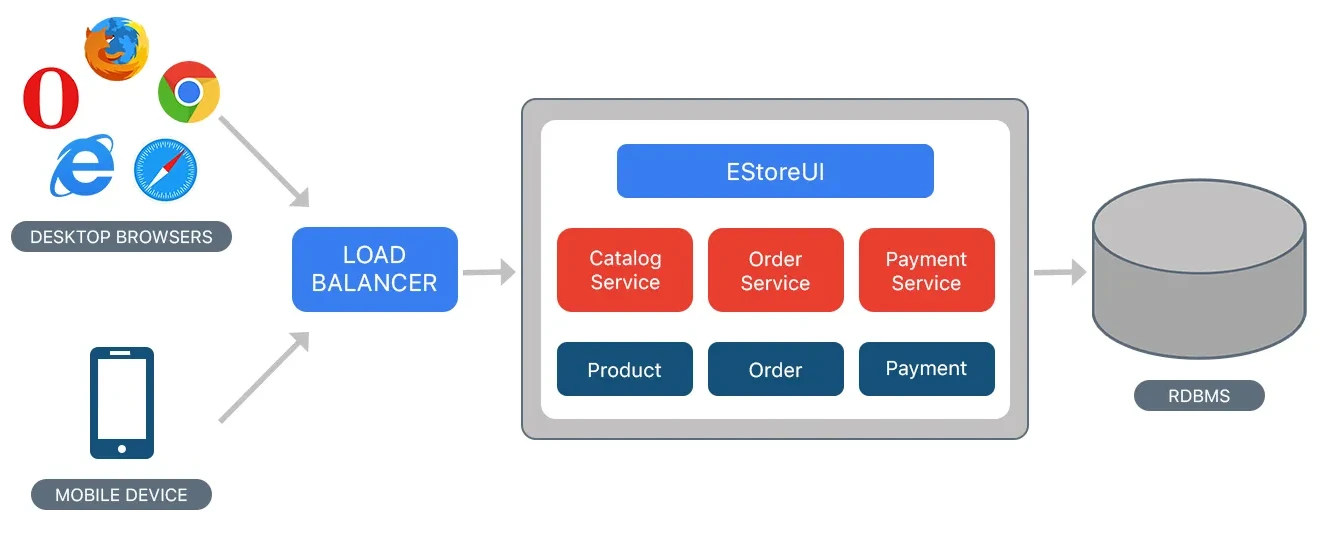
\includegraphics[width=\textwidth]{figures/monolith.png}
    \caption{Example of monolithic architecture, taken from \cite{siraj_ul_haq:intro_monolith_and_microservices}.}
    \label{fig:monolith_architecture}
\end{figure}

\subsection{Microservices}
\label{theory:microservices}
Kirsten Westende \cite{kirsten_westende:modular_monolith} described microservices architecture as an approach in which a large application is built as a suite of smaller services that are deployed independently.

Typically, each microservice has its own repository and a team of developers working on it. This enables a large company to be split into many small teams (single-digit teams) with agile development techniques.

Each microservice runs in its own process and communication with other services using protocols such as classic REST (HTTP/HTTP), gRPC, AMQP, and so on. These microservices are not (should not be) accessible directly by the client, but through an \textbf{API gateway} (reverse proxy) that routes traffic to the desired services. Services that are not stateless need to have a custom database and changes to the same object need to be propagated across the distributed system. 

\subsubsection{Benefits}
\begin{itemize}
    \item Productivity -- developers can understand small microservices much quicker and teams can take advantage of agile development, smaller services and smaller codebase also mean less stress on the developers' machines (faster IDE, fewer docker container dependencies, etc.).
    
    \item Scaling flexibility -- more demanded services can be scaled independently.
   
    \item Deployment -- new features and bug fixes do not affect deployment (and runtime) of~other services, also faster build times and independent deployments allow for multiple deployments a day.
    
    \item Technology flexibility -- each service can be developed using  a different technology stack, and use cases can be solved by languages that are better suited to the problem (i.e. python for AI use cases and so on) \dots large technological disparities could also be viewed as a disadvantage.
    
    \item Reliability -- isolation from other parts of the system makes it more difficult for the~entire system to crash due to bugs, DoS attacks etc.
\end{itemize}

\subsubsection{Drawbacks}
\begin{itemize}
    \item Debugging and Testing -- it is hard to test the integration of a microservice with other microservices and to catch bugs that originate from these scenarios. For integration testing, the entire test environment with all microservices needs to be set up.
    
    \item Distributed systems problems and complexity -- with microservices arise problems connected to distributed systems, such as understanding the system, dealing with data spread across several microservices, correctly handling data consistency through eventual consistency and so on. Complex topology may have the effect of not knowing which service is dependent on which (dependency hell), and thus be prone to cascading failures.
    
    \item Infrastructure complexity -- it could be challenging to manage the infrastructure of~a~microservice architecture, which must have a secure internal network and operate multiple databases, servers, containers (or even cluster), resulting in higher infrastructure costs as opposed to a monolithic architecture.
    
    \item Performance -- network calls between microservices bring high latency, not to mention the possibility of~losing communication packets, leading to even higher latency. 
    
    \item Reliability -- the system might be prone to \textbf{cascading failures} -- failure of a single microservice leading to a chain reaction of failures resulting in bringing down a large part or even the entire system.
\end{itemize}

\begin{figure} [H]
    \centering
    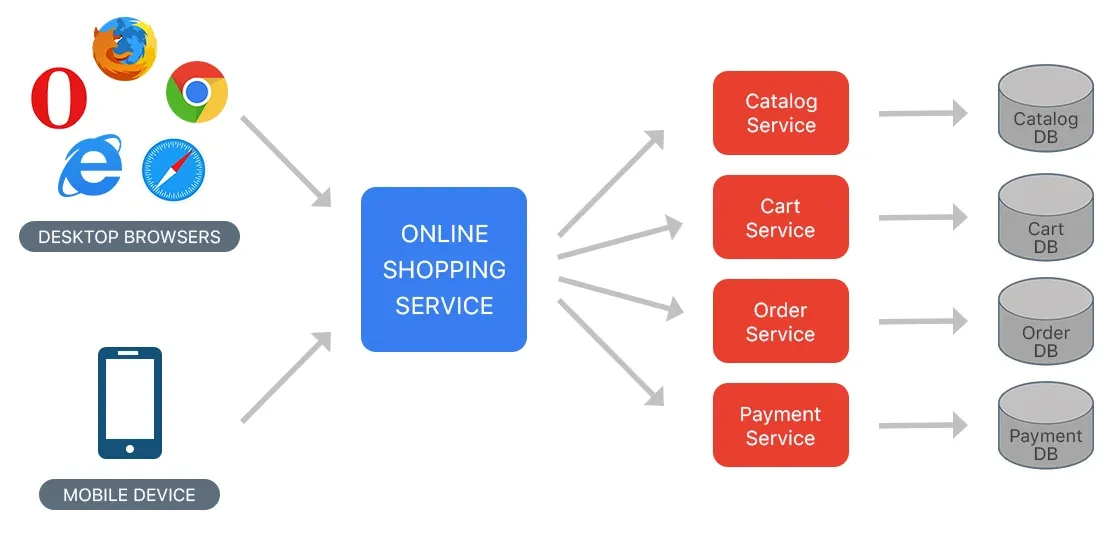
\includegraphics[width=\textwidth]{figures/microservices.png}
    \caption{Example of microservices architecture, taken from \cite{siraj_ul_haq:intro_monolith_and_microservices}.}
    \label{fig:micorservices_architecture}
\end{figure}

Microservices architecture is necessary for large companies (in the context of the number of developers) to enable hundreds of people to work on the system, but it is easy to misuse this architecture and design it poorly (see the next section \ref{fig:distributed_monolith}).

\subsection{Distributed monolith anti-pattern}
\label{theory:distributed_monolith}
A distributed monolith is an architecture which has distributed components, but these components (services) are tightly coupled with mutual calls all over the place (also known as \textbf{big ball of mud} anti-pattern), and therefore this monolith has the drawbacks of both the monolithic and microservices architecture. 

A distributed monolith usually results from a poorly designed microservices solution. That is why Martin Fowler \cite{martin_fowler:monlith_first} recommends starting the development of the system as a monolith first, even if using microservices would be worthwhile due to the scale of the application (aka \textbf{monolith-first strategy}). 

A distributed monolith can also be the result of poorly decomposed monolith, where the~original monolith was tightly coupled, and the distribution made it worse\dots~In this case a special monolithic architecture could be used that specializes for a system that would later need to migrate to microservices or gradually peel off services (see section \ref{theory:modular_monolith} about \textbf{Modular Monolith}).

A pragmatic approach should be used when choosing a system architecture, considering all the advantages and disadvantages for a given problem space.

\begin{figure} [H]
    \centering
    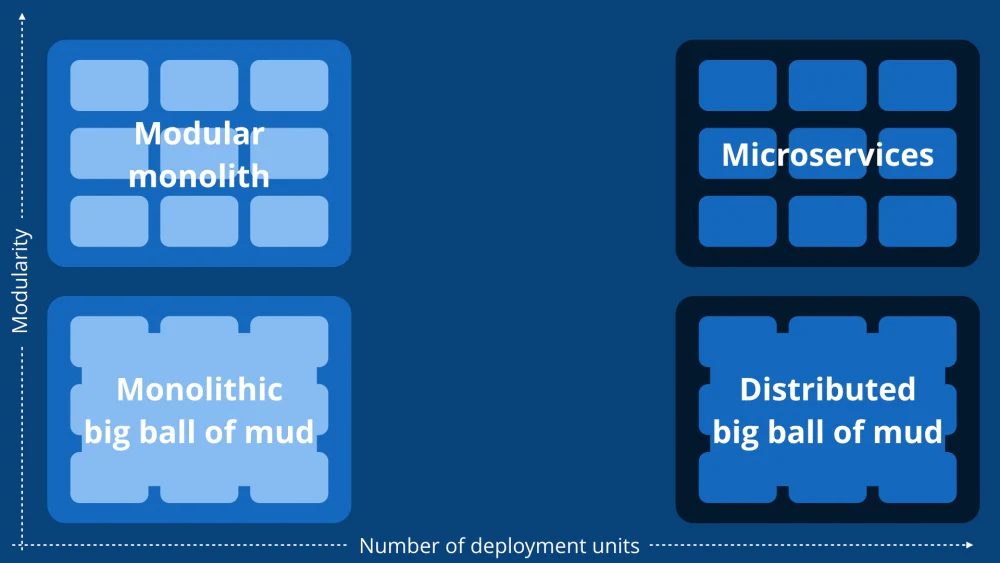
\includegraphics[width=\textwidth]{figures/dm.png}
    \caption{Diagram placing the types of architectures on the scale of modularity (y-axis) and distributability (x-axis). Taken from \cite{kirsten_westende:modular_monolith}.}
    \label{fig:distributed_monolith}
\end{figure}

\subsection{Domain Model}
Domain model describes selected aspects of an area of knowledge (aka the domain). It outlines key entities and objects, their relationships and rules within this problem area, providing a shared understanding for developers.

\subsubsection*{Anemic domain model}
\label{theory:anemic_domain_model}
The anemic domain model is a model where domain objects contain close to none business logic, this comes from the idea of separating data and logic. In this scenario, the consumer service is responsible for using the object in various business use-cases and the service is responsible for handling the anemic objects correctly (validations, calculations, business rules, \dots). Typically, an anemic object is a mirror of an entity stored in the database.

According to Martin Fowler \cite{martin_fowler:anemic_domain}, anemic domain model is an \textbf{anti-pattern} that contradicts with idea of objects-oriented design; which is to combine data and behaviour together. 

\subsubsection*{Rich domain model}
\label{theory:rich_domain_model}
Rich domain model is a contrary to the anemic domain model, hence the object associated logic is within the object itself, including validation and other business rules. Rich domain model brings cohesion and encapsulation and it can be reached by Domain-Driven Design (see \ref{theory:ddd}) or simply by object-oriented modeling.

\newpage
\section{Domain-Driven Design}
\label{theory:ddd}
Domain-Driven Design (hereinafter DDD) is an approach to software development that emphasizes understanding and modeling the business domain model. It focuses on collaboration between developers and \textbf{domain experts} to capture and implement a complex domain with complex business logic.

It was first introduced by Eric Evans in his book from 2003 \cite{eric_evans:ddd} where he described DDD through a catalog of patterns (described in sections \ref{ddd:strategy_design} and \ref{ddd:tactical_design}). Eric Evans also deemed as required to develop \textbf{ubiquitous language} for shared understanding of the domain and its concepts between developers and domain experts.

\subsection{Strategy Design}
\label{ddd:strategy_design}
The Strategy Design refers to the process of defining and modeling the high-level structure and organization of~the~modeled system. It is the first step in DDD developing process of~large domains and it emphasizes identifying and dividing domain into the \textbf{core domains}, \textbf{subdomains} and \textbf{bounded contexts}. By dividing the domain into these smaller pieces, we can easily build models for each piece, as opposed to large enterprise-wide domain where, according to Eric Evans \cite{eric_evans:ddd}, building one uniform model is not feasible or cost-effective.

\subsubsection{Subdomains}
The entire domain of the business organization is composed of smaller and more manageable  subdomains. There are 3 basic subdomains that need to be identified:
\begin{itemize}
    \item \textbf{Core Domain} -- refers to the central and most critical part of a business domain and the most important part for~the success of the organization (where the business gets its money or application gets its users, i.e. product catalog and order processing for~an~e-commerce application etc.).
    
    There can be more than one core subdomain and the significance of the core subdomain should come from the business side (not the user side) \dots~For example Facebook gets a lot of revenue from advertising, making it one of the core subdomains of Facebook.
    
    \item \textbf{Supporting Subdomain} -- models some aspect of the business that is essential, yet not core. The business creates a supporting subdomain because it is somewhat specialized (i.e. feedback and reviews in the context of an e-commerce application).
    
    \item \textbf{Generic Subdomain} -- captures nothing special to the business, but is required for~the~overall solution. Generic subdomains are common and standardized across the industry, solutions that could be applied with little adjustments already exist (i.e. payment processing, notifications etc.).
\end{itemize}

\begin{figure} [H]
    \centering
    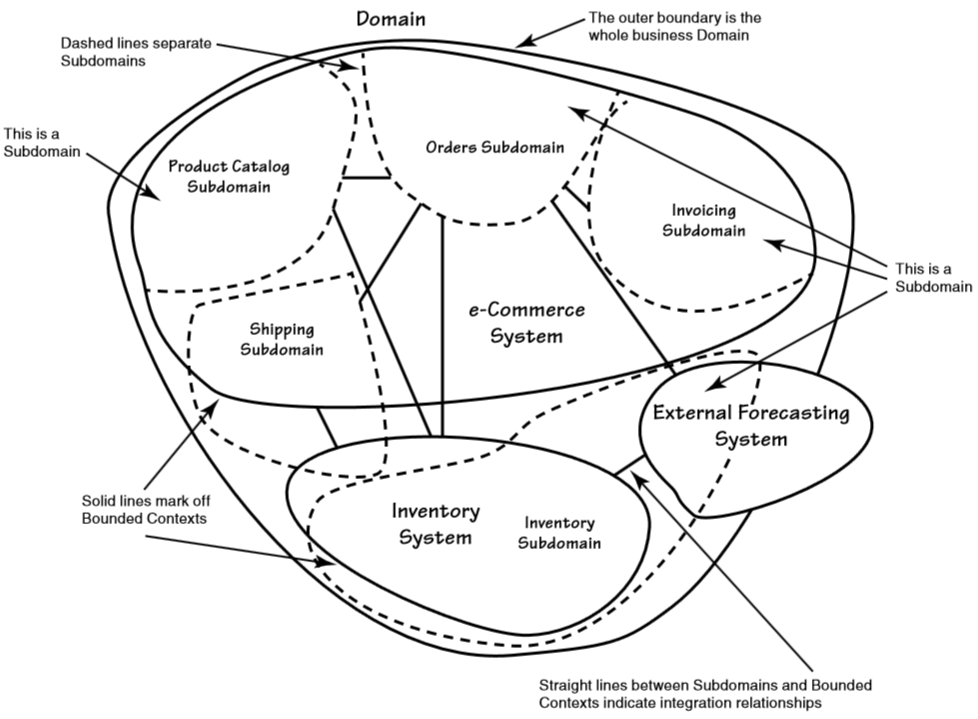
\includegraphics[width=1\textwidth]{figures/ddd-domain-sd-bc.png}
    \caption{Example of a domain with subdomains and bounded contexts, taken from \cite{vv:impl_ddd}.}
    \label{fig:ddd_domain_sd_bc}
\end{figure}

\subsubsection{Bounded Contexts}
Bounded context is a key concept in DDD and a central pattern in the strategy design. It helps with assigning explicit meaning to the terms used in the model for a certain scope, preventing ambiguity and misunderstandings -- common objects may have slightly or completely different meanings in different contexts (see figure \ref{fig:ddd_bc}); bounded contexts border and isolate these contexts. 

To help with duplication when it comes to the same objects in multiple bounded contexts, Eric Evans \cite{eric_evans:ddd} introduced the concept of \textbf{shared kernels}, where a shared kernel can contain shared objects from two bounded contexts on which the development teams of both models agree. Vernon Vaughn \cite{vv:impl_ddd} cautions and specifies that the~shared kernel should be small, and shared objects have special status and shouldn't be changed without consulting the~other team.

A single bounded context does not necessarily fall within the scope of a single subdomain, but can span across multiple subdomains -- as was illustrated in figure \ref{fig:ddd_domain_sd_bc}. From the~subdomains covered by the bounded context, it can be easier to determine which domain experts are needed to collaborate with a given development team.

\begin{figure} [H]
    \centering
    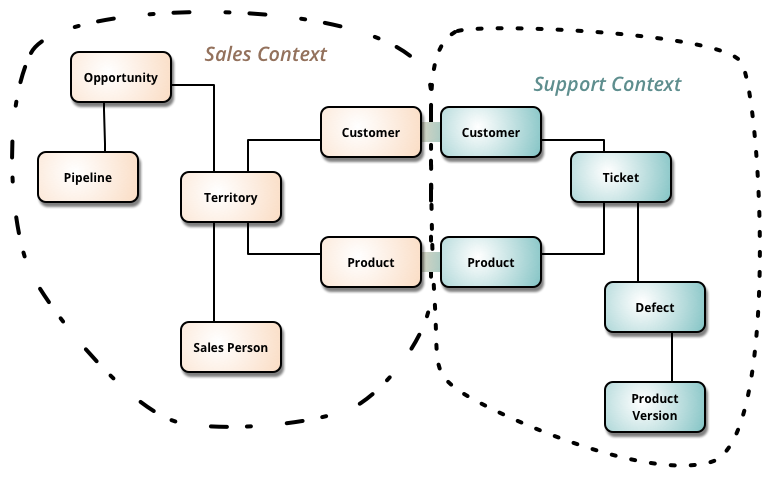
\includegraphics[width=0.9\textwidth]{figures/ddd-bc.png}
    \caption{Example of bounded contexts -- \texttt{Customer} and \texttt{Product} are objects that are both in \texttt{Sales Context} and \texttt{Support Context}, but could (and probably will) have a different meaning, taken from \cite{martin_fowler:bounded_context}.}
    \label{fig:ddd_bc}
\end{figure}

\subsubsection{Anti-corruption Layer}
On his blog, Nader Medhat \cite{nader_medhat:ddd_strategy_design} defines anti-corruption layer as a pattern for isolating a~bounded context (or a subsystem) from an external system that uses a different or incompatible language, architecture, or data structure.

An anti-corruption layer is typically implemented as a set of service, interfaces and adapters that are placed between systems and translate external data/behavior into compatible form with the local system, and vice versa.

\begin{figure} [H]
    \centering
    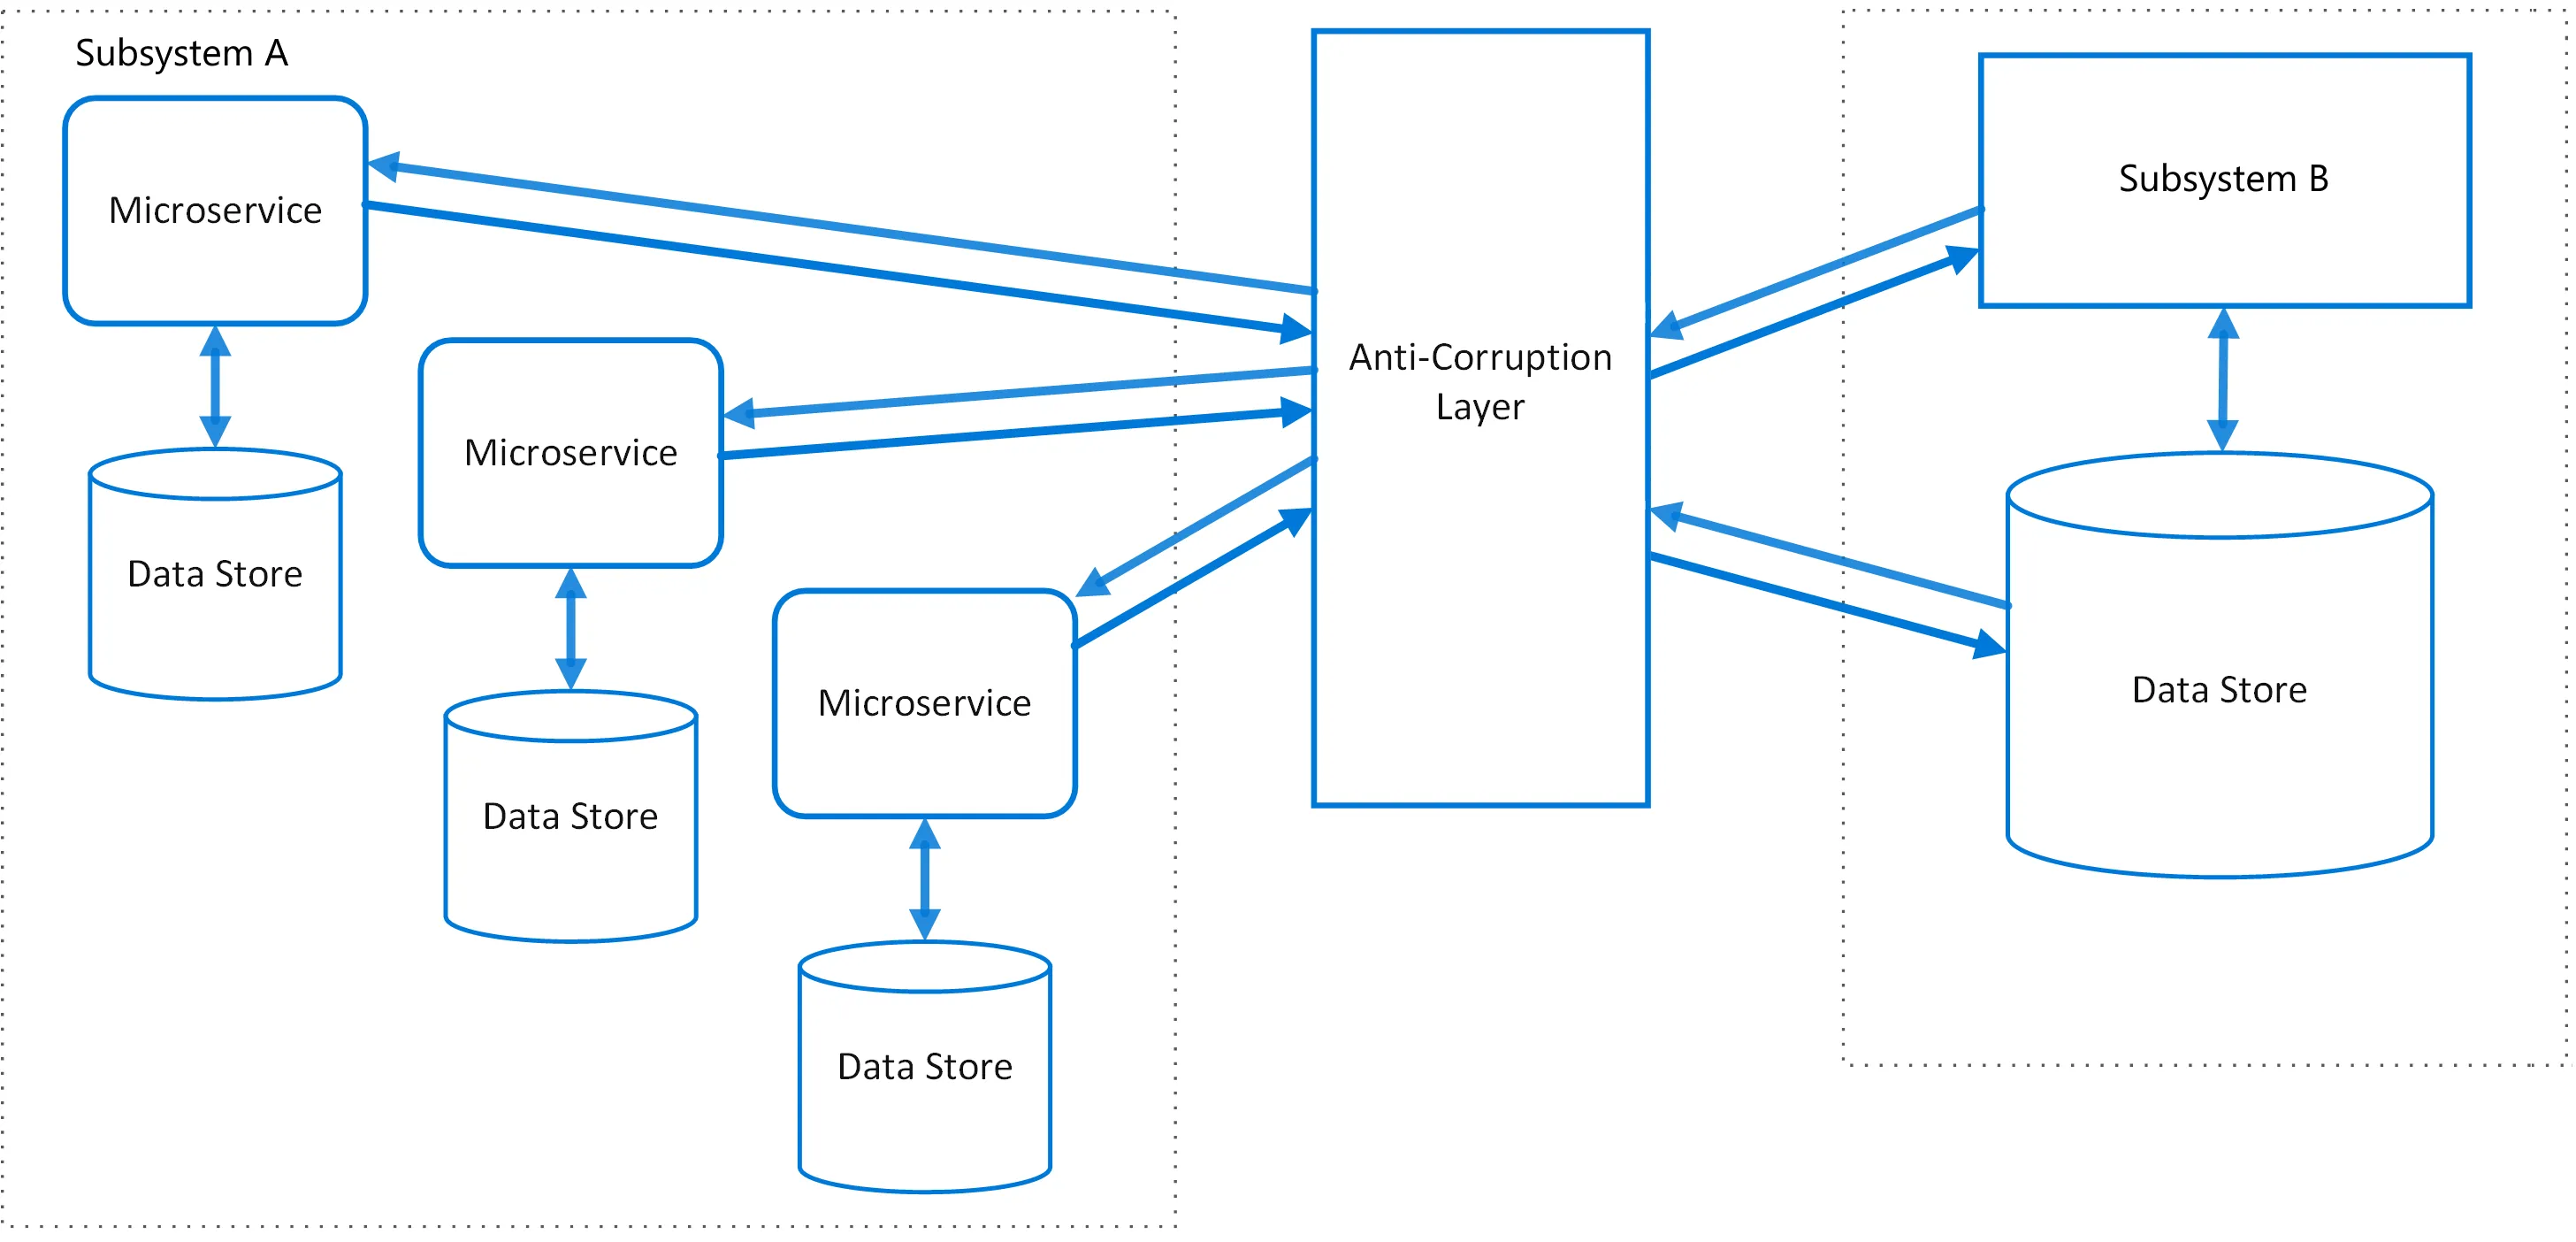
\includegraphics[width=0.9\textwidth]{figures/acl.png}
    \caption{Example of an anti-corruption layer, taken from \cite{nader_medhat:ddd_strategy_design}.}
    \label{fig:ddd_acl}
\end{figure}

\subsection{Tactical Design}
\label{ddd:tactical_design}
The tactical design is a set of design patterns used in the construction of the domain of~a~single bounded context. These patterns are the fundamental building blocks of~a~domain model and they help to avoid designing the domain as a \textbf{big ball of mud}\footnote{\url{https://en.wikipedia.org/wiki/Anti-pattern\#Big\_ball\_of\_mud}} (figure \ref{fig:bug_ball_of_mud}).

\begin{figure} [H]
    \centering
    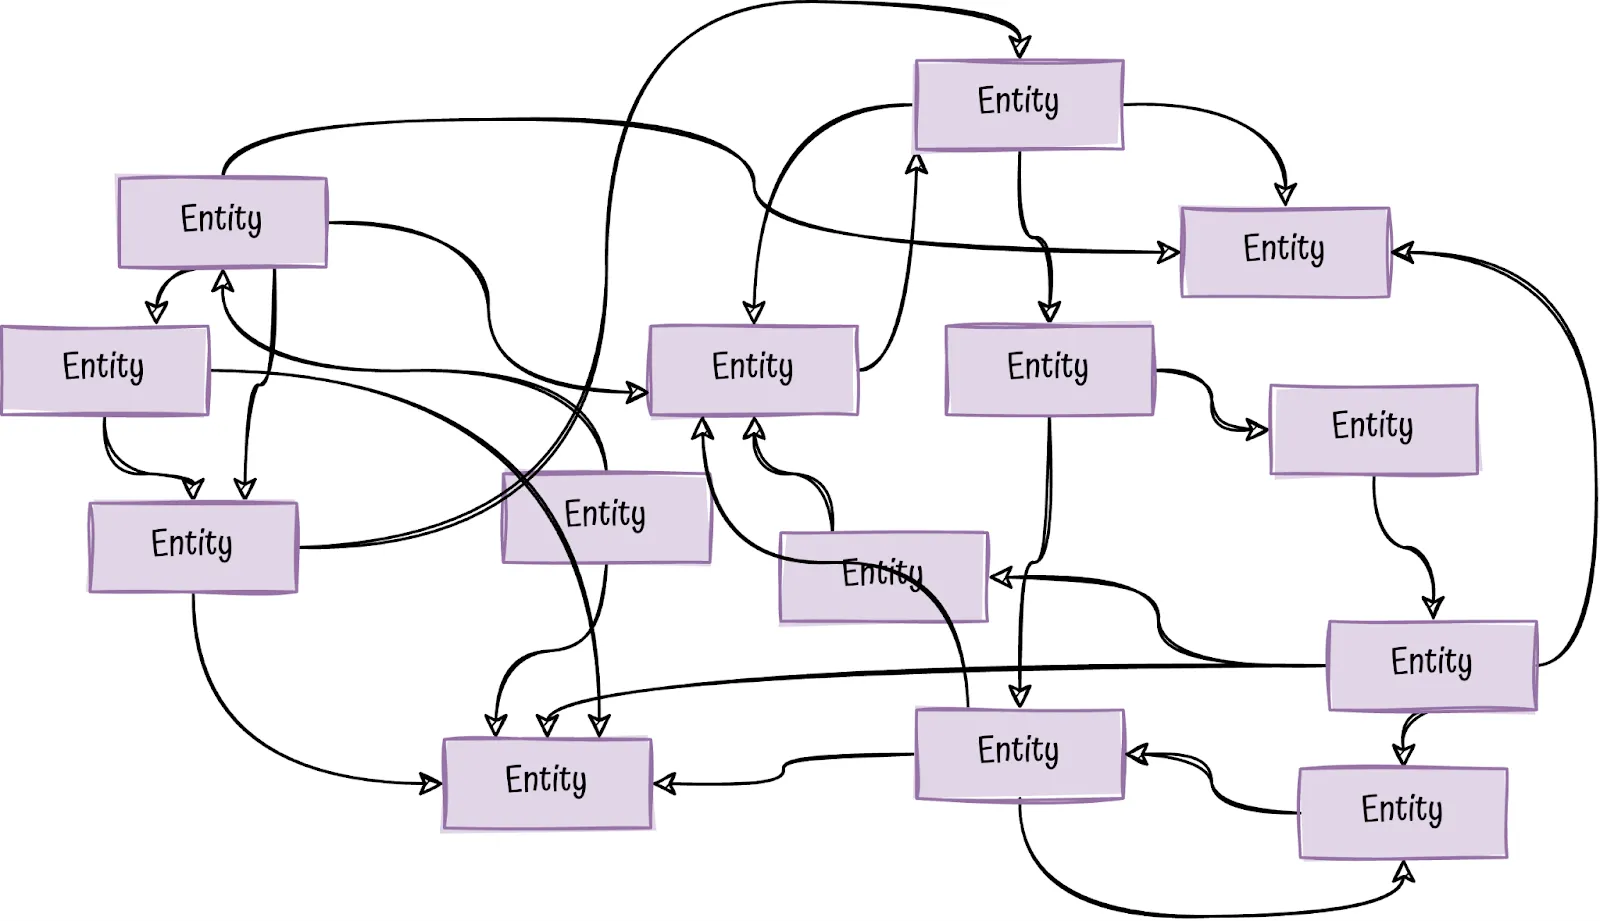
\includegraphics[width=\textwidth]{figures/bbom.png}
    \caption{Complex graph of entities connected to each other, a software anti-pattern also known as big ball of mud. Taken from \cite{albert_llousas:design_ddd_aggregates}.}
    \label{fig:bug_ball_of_mud}
\end{figure}

\subsubsection{Entities \& Value Objects}
\label{ddd:entities_and_value_objects}
According to Eric Evans \cite{eric_evans:ddd}, an entity is an object primarily defined by its identity (Id). If non-identifying attribute of an entity changes (i.e. a product gets cheaper), it is still the~same entity, therefore comparing two Entities should be done by comparing their Ids.

Unlike entities, value objects have no identity, but they describe some characteristic (i.e. Color). If any of the attributes of a value object change, the entire value object describes this characteristic as a new fact (i.e. red attribute of RGB Color changes), therefore the~value object should be \textbf{immutable} and the comparison should be done by comparing all attributes of the value object.

\newpage
\subsubsection{Aggregates}
\label{ddd:aggregate}
To quote Eric Evans \cite{eric_evans:ddd}, \textit{``an aggregate is a cluster of associated objects that we treat as~a~unit for the purpose of data changes''}. Each aggregate has a its \textbf{aggregate root} (single entity) which serves as an interface for modifying objects that are within the aggregate boundary. The root entity is the only object inside the aggregate that can be referenced by objects outside the aggregate boundary.

The aggregate root is the only object that can modify objects inside the aggregate boundary so that the aggregate root can enforce \textbf{invariants}, which Vaughn Vernon \cite{vv:impl_ddd} describes as~business rules that must always be consistent and cannot be broken, therefore:

\begin{itemize}
    \item models cannot be created if any invariant is broken  -- ensured by creator (factory method or factory, alternatively constructor);
    \item models cannot be modified if any invariant is broken -- ensured by modifying data using public methods of the aggregate root.
\end{itemize}

With this in mind, it is necessary to always retrieve the entire aggregate from the database, otherwise the aggregate root may incorrectly evaluate the business rules. This implies that the aggregate should be as small as possible to minimize large data transfers.

A typical example is an order and its line items. Although line items are separated objects, together with an order they would be treated as a single aggregate, with the order serving as the aggregate root for data changes.

\begin{figure} [H]
    \centering
    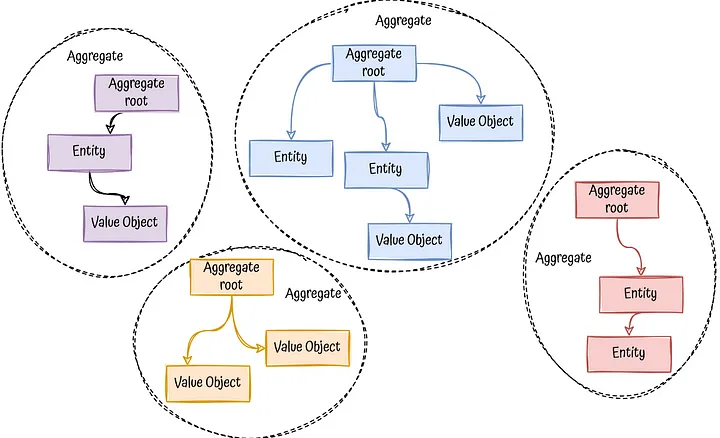
\includegraphics[width=\textwidth]{figures/aggregates.png}
    \caption{Domain modeled using DDD aggregates. Taken from \cite{albert_llousas:design_ddd_aggregates}.}
    \label{fig:ddd_aggregate}
\end{figure}

\newpage
\subsubsection{Domain Events}
 A domain event is something that happened in the domain that other parts of the domain need to be aware of. An event is a domain object that holds necessary data for event consumers to properly react -- i.e. \texttt{UserCreatedDomainEvent} should hold user identifier (id/email/\dots) and possibly other needed data (date, nationality, etc.).
 
 Using domain events provides a loosely coupled and a highly cohesive model, which is crucial for designing modular systems.

The main use case for domain events is to propagate changes between aggregates, where publishing, as defined in Microsoft's book on microservices \cite{ms:microservices}, can be done via 2 options:
\begin{enumerate}
    \item[A)] Right \textbf{before} committing data to the database (this makes a single transaction including side effects from the event, possibly spanning across multiple aggregates).
    \item[B)] Right \textbf{after} committing data to the database (this makes multiple transactions and a~necessity to handle eventual consistency and compensatory actions for failures).
\end{enumerate}

Many DDD authors, including Eric Evans \cite{eric_evans:ddd} and Vaughn Vernon \cite{vv:aggregates}, advocate rule that one transaction = one aggregate, thus publishing should be done via option B.

Microsoft's book on microservices \cite{ms:microservices} explains the~idea of option B by claiming that the~number of database locks will be substantial in large-scale applications with high scalability needs and atomic changes are often not needed by the business.

However, Jimmy Bogard \cite{jimmy_bogard:domain_events} argues that it is justifiable to span a single transaction across multiple aggregates if those aggregates are related to the side effects for the same original command, thus taking advantage of Option A and strong consistency.

Another use case for a domain event is to apply the operation side effects (i.e. sending email, pushing notifications, etc.). These side effects do not access the database but call other services, so publishing needs to be asynchronous outside of the database transaction with a little bit of tweaking so that the side effects do not apply if the transaction fails, this can be done using an \textbf{outbox pattern} (see \ref{theory:outbox}).

Domain events can also be used to propagate committed transaction changes to different bounded contexts -- modules/microservices (eventual consistency), in which case the domain event is called an \textbf{integration event} (as defined in Microsoft's book on microservices \cite{ms:microservices}). Publishing integration events should always be asynchronous, hence it is usually solved using an outbox pattern and an event bus/message-broker. This is often used with \textbf{Event Sourcing}\footnote{\url{https://martinfowler.com/eaaDev/EventSourcing.html}} and \textbf{Event-Driven Architecture}. 

\subsubsection{Domain Services}
Vernon Vaughn \cite{vv:impl_ddd} characterized a domain service as a stateless operation that fulfills a~domain-specific task. The domain service provides means to handle operations, that naturally does not belong to any of the entities or value objects. The interface of the~domain service is defined in~terms of other elements of the~domain model (the contracts are part of~the~domain model).

An example of a domain service could be a \texttt{DiscountCalculator} service, in the context of an e-commence application. The order aggregate root would handle aggregate specific business rules (adding line items, calculating total price, etc.), but could not handle discount calculations, because it requires additional data that are not available in the order aggregate -- user aggregate details, such as account type (standard/premium), student discounts (ISIC), etc. Calculating discount has business logic that requires access to several aggregates, making it a good candidate for a domain service.

As described in the section \ref{theory:anemic_domain_model}, handling all business logic in domain service would result in an anemic domain model, which is considered an anti-pattern, and DDD aims for a~rich domain model (see \ref{theory:rich_domain_model}), therefore it is necessary to consider each use of the domain service.

\subsubsection{Repositories}
The repository pattern is a widely used design pattern outside of DDD. The repository provides an interface for acquiring references to already existing domain objects persisted in~the~database and storing new domain objects. Repositories decouple the~domain from the~persistence technology (one or more database strategies and data sources, etc.). Another benefit mentioned by Eric Evans \cite{eric_evans:ddd}, is the possibility to use dummy in-memory collections for easy testing at the beginning of a project.

Ideally, the domain model should contain only repository interfaces with the contracts specified in the domain. Repository implementations should reside elsewhere, for example in the infrastructure or persistence layer.

\subsubsection{Factories}
The factory pattern, belonging to the Gang of Four's Creational design patterns,  offers encapsulation for the creation of the domain objects. Eric Evans \cite{eric_evans:ddd} recommends using factory when the creation of an object, or an entire aggregate, becomes complicated or reveals too much of the internal structure. Factory can enforce invartiants and use services (repositories, domain services, infrastructure services, \dots), injected via DI (see \ref{theory:DI}), to~resolve more complex business rules.

Alternatively, if creating a domain object does not require additional services, it is preferable to use the \textbf{factory method} design pattern, which is a static method on the objects themselves. This provides means for enforcing invariants and returning a null reference if an invariant is broken.

Constructors of targeted objects should be accessible only from factories and factory methods, so that the object creation cannot be done incorrectly:
\begin{itemize}
    \item When using factory methods, objects should have private constructors.
    
    \item Factories are harder to solve since programming languages do not provide ways to~restrict method access only to one class. Maximum language capability should be used to restrict the access (internal to the assembly etc.) and additional means could be added, such as custom code analyzers or tests for incorrect object creation.
\end{itemize}

\section{Monolithic architectures}
\label{theory:monolith_architectures}

There are many monolithic architectures, Robert C. Martin mentions in his blog \cite{robert_martin:ca_blog} that all architectures\footnote{He was referring to the 6 architecture examples that he had listed, but it should generally apply to all.} have the same objective, which is the separation of concerns and production of systems that are:
\begin{itemize}
    \item Independent of frameworks.
    \item Testable business rules without UI, Database, Server and other external elements.
    \item Independent of UI -- frontend can be replaced with a console application without changing the business logic.
    \item Independent of Database -- Database could be swapped for other database providers or even database types (i.e. SQL to NoSQL).
    \item Independent of any external agency -- business logic does not know anything about the outside world.
\end{itemize}

This is accomplished by dividing the code into layers/modules, specifying what each layer should contain and solve, and defining strict dependency rules between them.

\subsection{Layered Architecture}
\label{theory:layered_architecture}
The layered or N-layered architecture splits the code into 3 layers (or more), where each layer can only depend on the lower layers. Most of monolithic architectures are based on layered architecture and are in some form layered architecture, just with more strict rules/rearranged layers/slightly different component placement etc.

\begin{figure} [H]
    \centering
    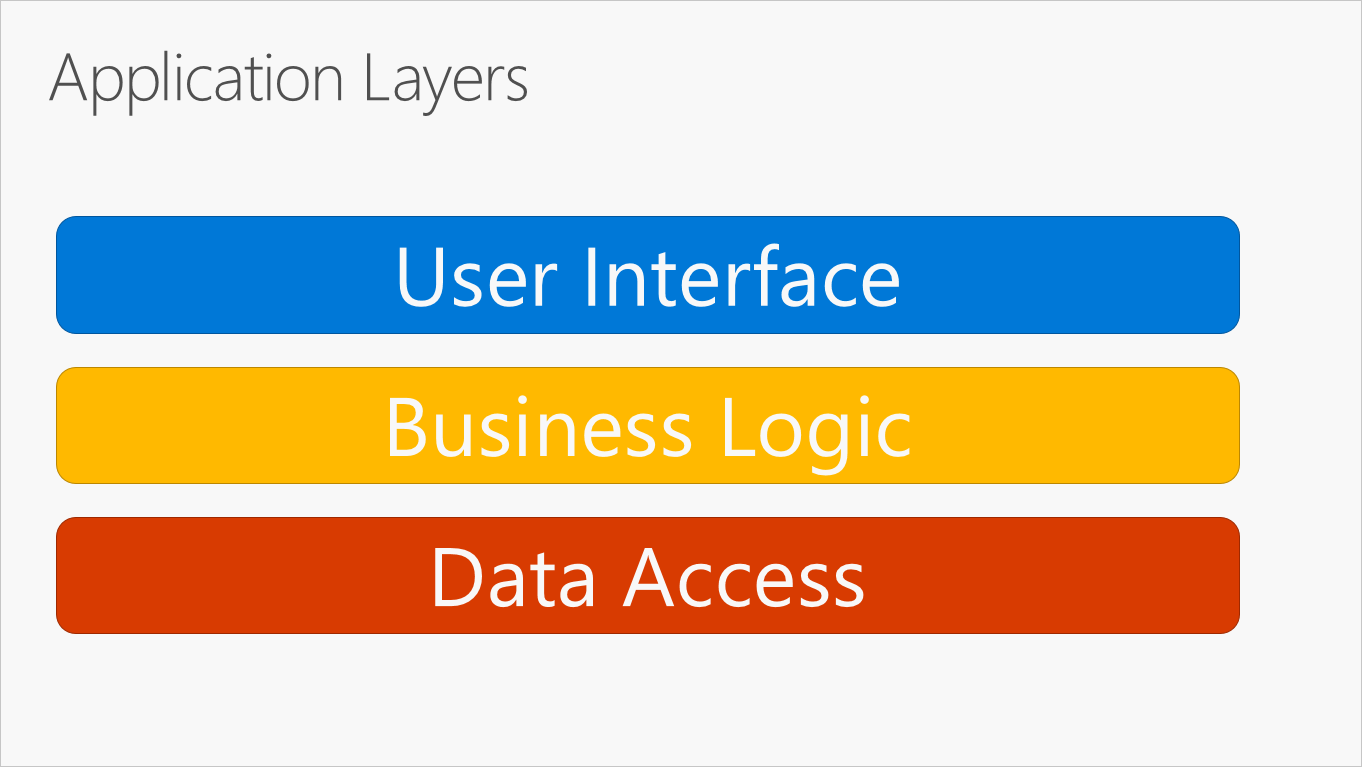
\includegraphics[width=0.9\textwidth]{figures/layered-architecture.png}
    \caption{Architecture diagram of the tradition 3-layered architecture, taken from \cite{ms:modern_webapps}.}
    \label{fig:arch:layered_architecture}
\end{figure}

Typical layered architecture decomposes system into layers as follows:
\begin{itemize}
    \item Presentation Layer -- presents the system to the client in form of a UI or an API (Rest, gRPC, GraphQL, \dots).
    \item Business Layer (BL) or Business Logic Layer (BLL) -- encompasses application business logic (services, facades, potentially mappers, DTOs and so on).
    \item Data Access Layer (DAL) or Data Layer (DL) -- contains data specific system parts such as entities, repositories, migrations \dots and connection to the database.
\end{itemize}

There could be additional layers to extract some componests for better applicability and reusability, for example layer with API contracts (DTO requests and responses) or layer for common objects and interfaces (i.e. \texttt{IDateTimeProvider}, a result pattern and so on).  

In my experience, the layered architecture often results in an anemic domain model (see \ref{theory:anemic_domain_model}) as it encourages to have domain objects as anemic data objects in DAL and business logic in services in BL, and is therefore not a good candidate for DDD.

\subsection{Clean Architecture}
\label{theory:clean_architecture}
Clean Architecture, defined by Robert C. Martin \cite{robert_martin:clean_architecture}, is an architecture emerging from Onion Architecture (and some others) as it splits the system into concentric circles (layers).

As with the layered architecture, Clean Architecture has a dependency rule pointing inwards (see figures \ref{fig:arch:clean_architecture} and \ref{fig:arch:modern_clean_architecture}), meaning the inner layers cannot depend on the outer layers.

\begin{figure} [H]
    \centering
    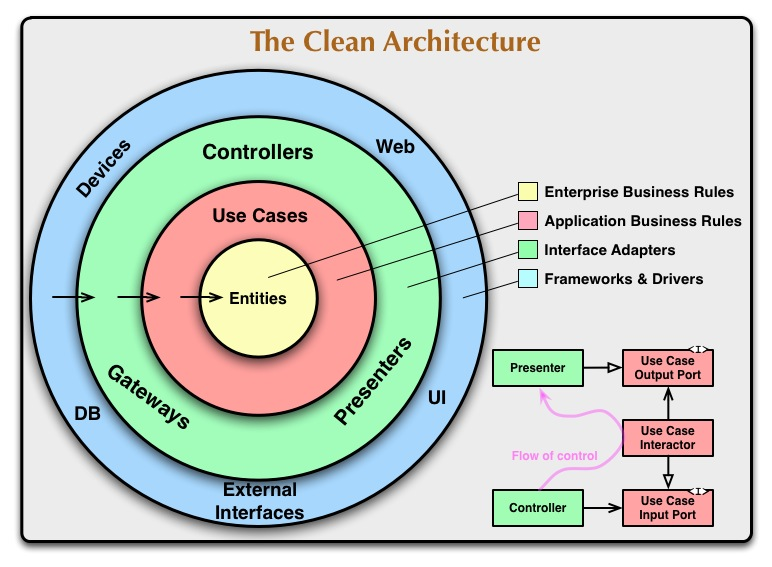
\includegraphics[width=0.9\textwidth]{figures/clean-architecture.jpg}
    \caption{Architecture diagram of the Clean Architecture by Robert C. Martin \cite{robert_martin:clean_architecture}.}
    \label{fig:arch:clean_architecture}
\end{figure}

\begin{figure} [H]
    \centering
    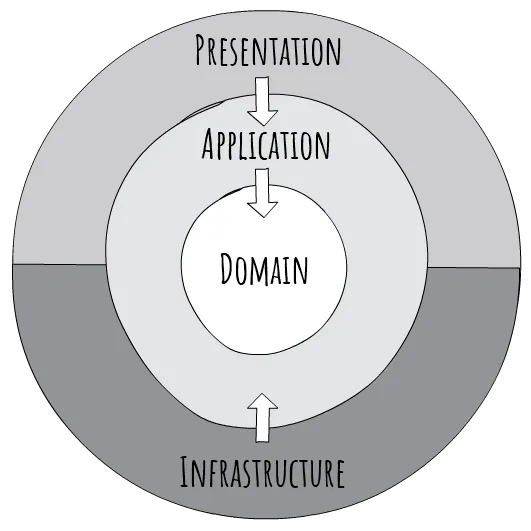
\includegraphics[width=0.65\textwidth]{figures/mod-clean-architecture.png}
    \caption{Another view at the Clean Architecture, taken from \cite{dorin_baba:clean_architecture}.}
    \label{fig:arch:modern_clean_architecture}
\end{figure}

A more popular view at Clean Architecture, illustrated in figure \ref{fig:arch:modern_clean_architecture}, is as follows:
\begin{itemize}
    \item Presentation Layer -- is an application entry point, contains components necessary for presentation to the client, it can be API endpoints (REST, gRPC etc.), MVC architecture (Controllers and Views) or components of more advanced frameworks enabling both SSR (Server-side rendering) and CSR (Client-side rendering).
    
    \item Application Layer -- includes the handling of application use-cases, that is, services or queries/commands and their handlers if used with CQRS pattern (see \ref{theory:CQRS}).
    
    \item Domain Layer -- is the core of the system, holds all the business logic of the domain and emphasizes rich domain design (see \ref{theory:rich_domain_model}).
    
    \item Infrastructure Layer -- is often divided into infrastructure and persistence, consists of~infrastructure-specific code such as integration with database, message broker, mail sender, 3rd party APIs and so on.
\end{itemize}

\subsection{Vertical Slice Architecture}
\label{theory:vertical_slice_architecture}
Layered architectures organize the system around technical layers and the cohesion between layers is low, leading to changes in many layers as features are added. The vertical slice architecture introduced by Jimmy Bogard \cite{jimmy_bogard:vertical_slice_architecture} addresses this problem by organizing code around vertical slices, where each slice represent an application feature (use case). 

The key for vertical slice approach is to minimize coupling between slices, and maximize coupling inside a slice. Therefore, new features should only add code without changing the~shared code and worrying about side effects. The vertical slice architecture naturally comes with CQRS (see \ref{theory:CQRS}), as it already separates the code into features where the~feature is a Command or a Query. 

\begin{figure} [H]
    \centering
    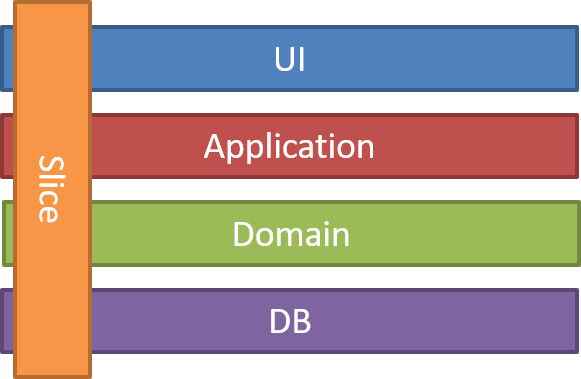
\includegraphics[width=0.8\textwidth]{figures/vertical-slice-architecture.png}
    \caption{Architecture diagram of a vertical slice architecture, taken from \cite{jimmy_bogard:vertical_slice_architecture}.}
    \label{fig:arch:vertical_slice_architecture}
\end{figure}

An example of an application structure using the vertical slice architecture with CQRS: \vspace{6pt}

\dirtree{%
.1 ProjectManager/.
.2 Entities/.
.2 Features/\DTcomment{directory with vertical slices}.
.3 Projects/.
.4 GetProject/.
.5 GetProjectEndpoint.cs.
.5 GetProjectQuery.cs.
.5 GetProjectQueryHandler.cs.
.5 \dots.
.4 CreateProject/.
.5 CreateProjectEndpoint.cs.
.5 CreateProjectCommand.cs.
.5 \dots.
.3 \dots.
.2 Middlewares/.
.2 Program.cs.
.2 \dots.
}

Noteworthy from the example is the \textbf{vertical approach to naming} and structuring  directories, which allows developers easier/faster understanding of the code as it outlines what the application does and what features it has.

The main downside mentioned by Jimmy Bogard \cite{jimmy_bogard:vertical_slice_architecture} is that this approach does assume that the team understands code smells and refactoring. 

\subsection{Modular Monolith}
\label{theory:modular_monolith}
The modular monolith (sometimes called majestic monolith) is a monolith designed with an~emphasis on interchangeable, independent (and potentially reusable) modules, whereby the architecture seeks to gain benefits from both monolithic and microservices architectures. 

By Kirsten Westeinde's definition \cite{kirsten_westende:modular_monolith}, \textit{``A modular monolith is a system where all of~the~code powers a single application and there are strictly enforced boundaries between different domains.''} The \textbf{strict boundaries} between the modules are the essence of the modular monolith architecture.

The modular monolith is composed of \textbf{loosely coupled modules}, where modules represent cohesive sets of functionalities and are independent of each other (similar to microservices). Modules may mirror sub-domains/bounded contexts of the DDD. Example of module may be payments module, shipping module, booking module etc.

This is very similar to microservices and therefore it is easy to transition from a modular monolith to a microservice architecture. Main benefit is the ability to gradually transition and extract modules one by one, f.e. if a module faces high demand, it is easy to peel off this module into standalone microservices and scale it separately.

Separating a system into modules brings more microservice-like way of developing and maintaining the system while retaining the ease of testing and debugging.

It should be noted that when the system starts to be decomposed into microservice, the~system looses the characteristics of easy debugging and integration testing. 

\begin{figure} [H]
    \centering
    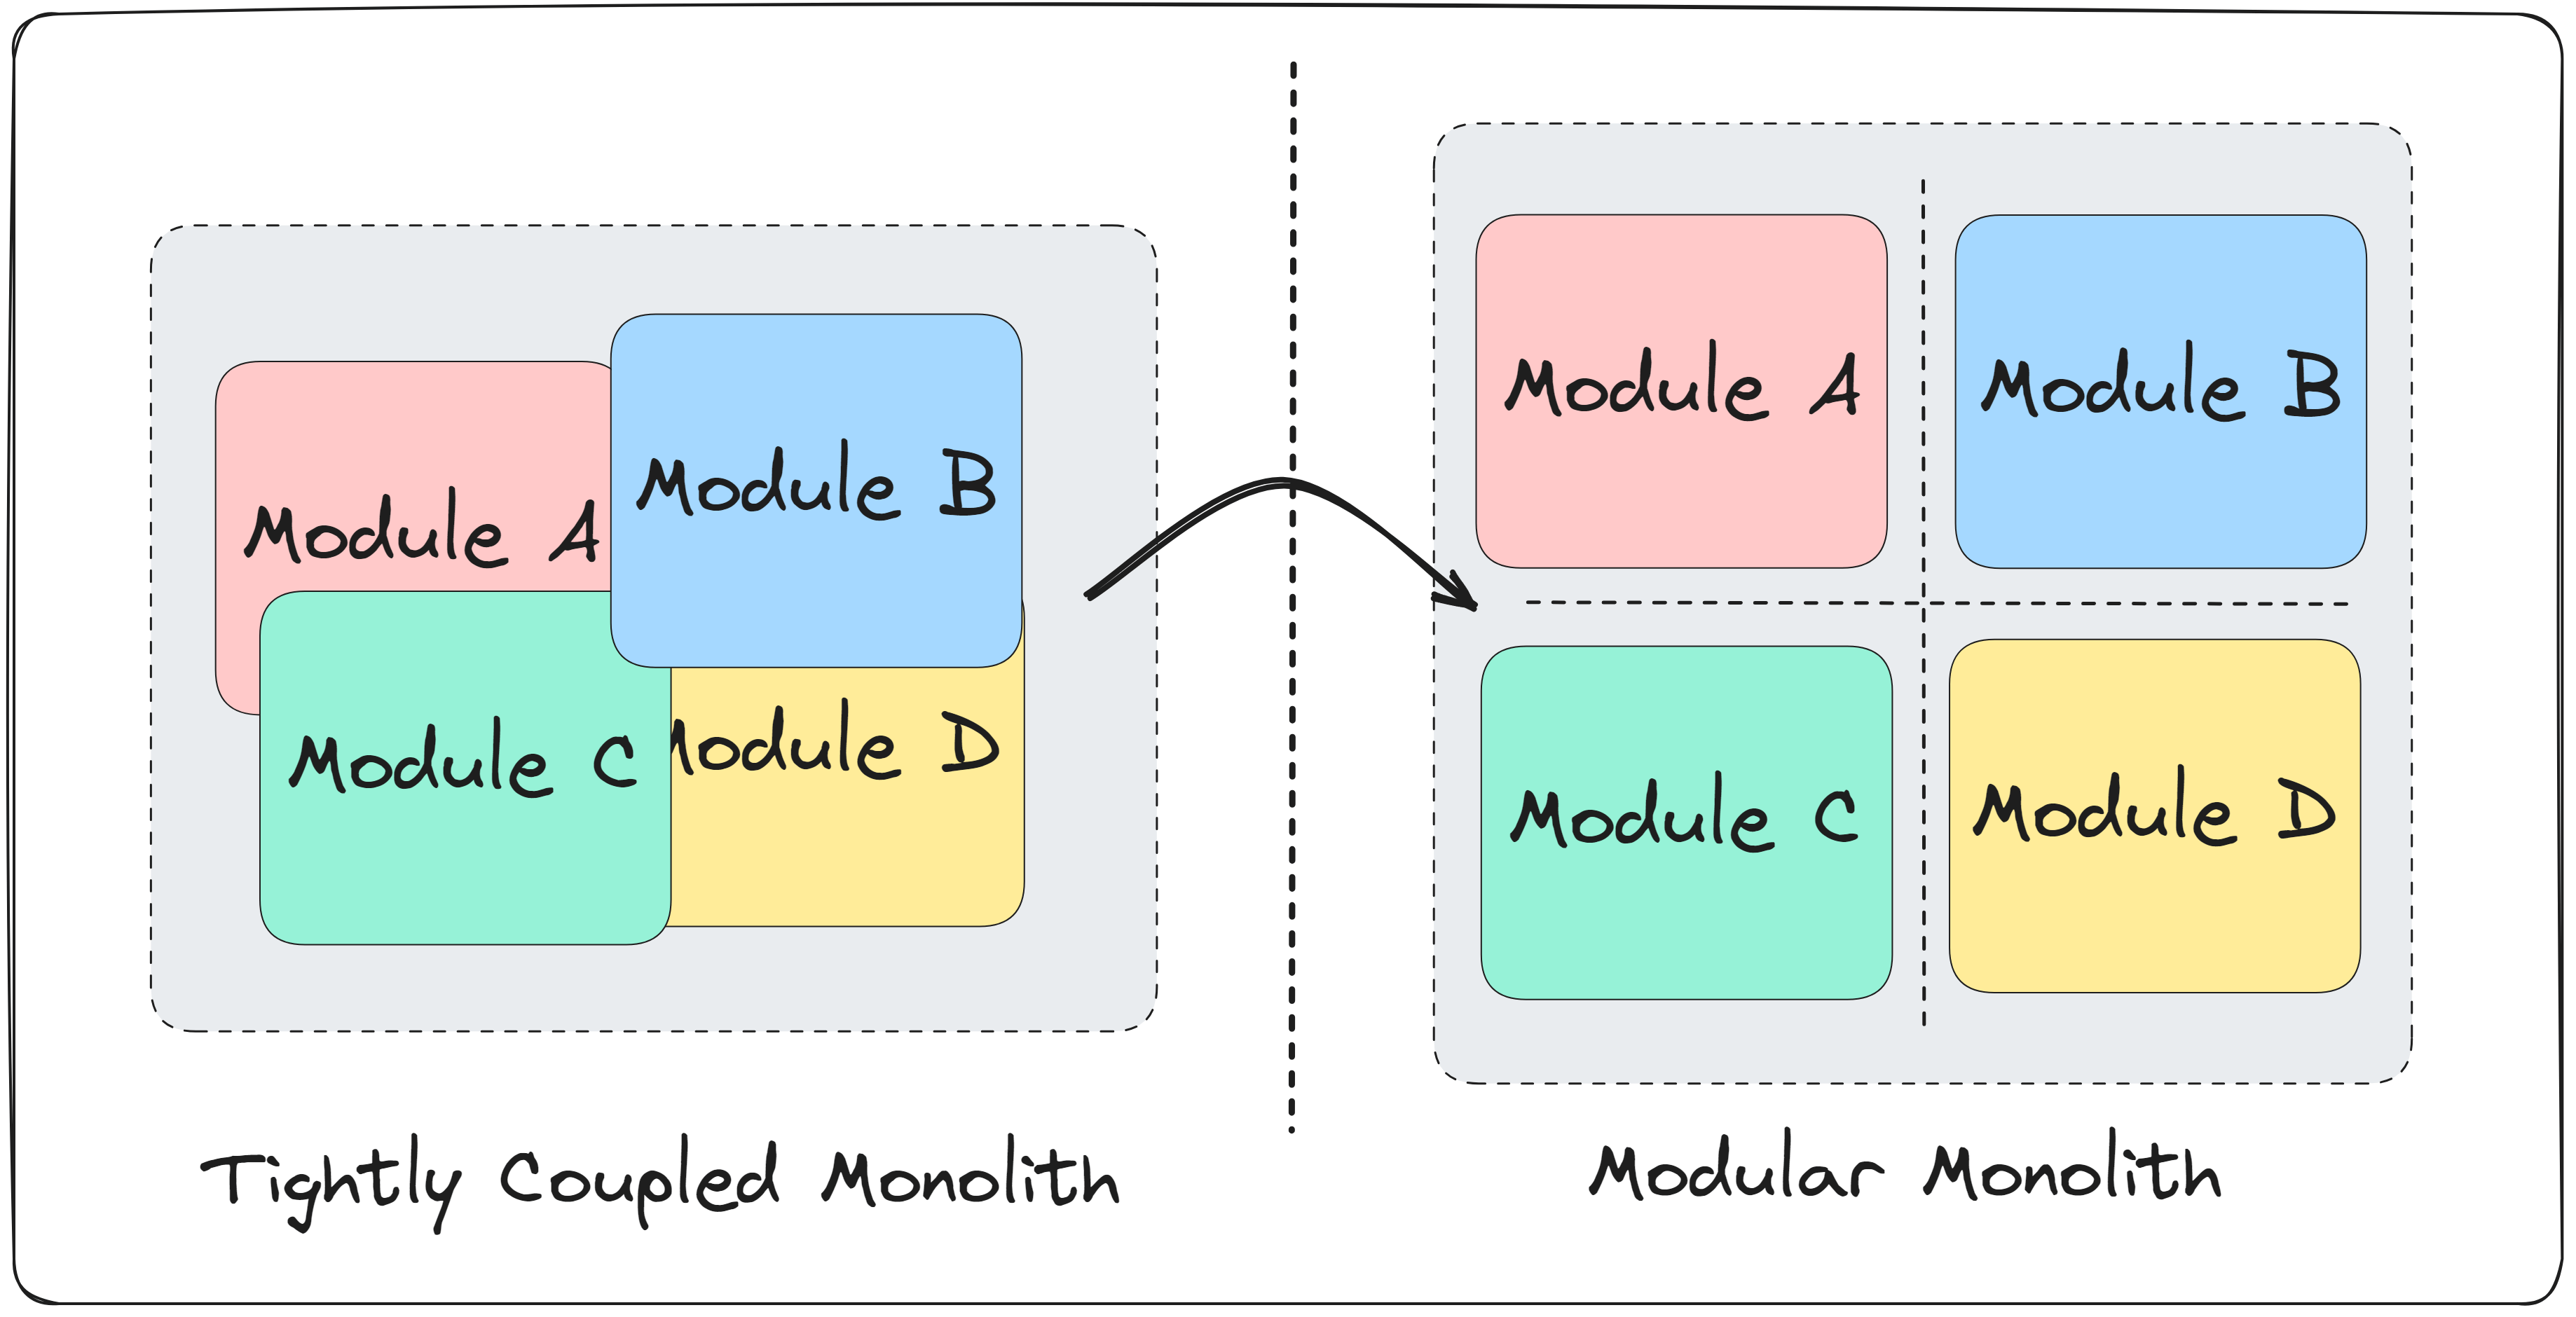
\includegraphics[width=\textwidth]{figures/m_to_mm.png}
    \caption{Diagram showing decoupling of a monolith into modules, taken from \cite{milan_jovanovic:modular_monolith_communication_patterns}.}
    \label{fig:arch:m_to_mm}
\end{figure}

\subsubsection{Communication between modules}
When separating modules, it is necessary to define how the modules should communicate, Milan Jovanović in his blog post \cite{milan_jovanovic:modular_monolith_communication_patterns} specified 2 types of communication patterns between modules -- \textbf{Method Calls} (synchronous) and \textbf{Messaging} (asynchronous).

The first and simpler approach is to communicate by calling methods of the public API (interfaces) exposed by each module. The modules are then dependent on other modules' APIs at compile-time and DI will provide their implementation at run-time. The advantages of of this approach are speed (fast in-memory calls) and easy implementation. The~disadvantage is the \textbf{strong coupling} between modules. 

The second approach is to introduce an indirection layer in the form of a \textbf{message broker}. The modules communicate with each other by sending messages in the fire-and-forget fashion and subscribing to the relevant messages in their context. Modules know nothing about other modules and depend only on \textbf{message contracts}. This solves the coupling problem, but has some drawbacks, such as increased complexity.

\subsubsection{Data isolation}
Milan Jovanović \cite{milan_jovanovic:modular_monolith_data_isolation} mentioned that the modular monolith has strict rules for data integrity:
\begin{itemize}
    \item Each module can only access its own tables.
    \item No sharing of tables or objects between modules.
    \item Joins are only allowed between tables of the same module.
\end{itemize}

The modules should be self-contained and each module should handle its own data. Other modules can access this data using the module's public API, this data isolation could be handled on 4 levels of separation:
\begin{itemize}
    \item Separate Table -- basically zero separation, tables for each module live inside one database. It may be hard to determine which tables belong to which module.
    \item Separate Schema -- each module has its own database schema containing all the modules tables.
    \item Separate Database -- each module has its own database in which resides all of the~module's data. This level of separation forces developers to solve any coupling problems, resulting in a microservices-style of separation and providing an easy way to extract modules.
    \item Different Database Type -- each module may have different database types (relational, document, graph etc.), this level of separation is the same as in a microservices architecture and it might be forced by business needs.
\end{itemize}

\subsubsection{Real world example}
Roberta Arcoverde, Director of Engineering at \textbf{Stack Overflow}, in the podcast interview with Scott Hanselman \cite{roberta_arcoverde:stackoverflow_mm} reveled aspects of the stack overflow architecture. 

One of 9 stack overflow servers handles 6000 request per second and whole system handles roughly 2 billion page requests per month. The system is designed for low latency and rendering a page takes about 12 milliseconds.

Surprisingly, despite this high demand and need to scale, stack overflow does not use microservices  (and they neither run in the cloud), but uses a modular monolith architecture. Roberta Arcoverde mentioned in the podcast that the question of migrating to microservices has been brought up many times, but they have never come up with the pragmatic benefits because they do not straggle with the typical monolithic disadvantages:
\begin{itemize}
    \item Roberta Arcoverde mentioned good \textbf{time to merge} metric in the context of maintainability and developer productivity.
    \item High demand is not a problem with the monolithic approaches to scaling and high degree of cashing on the database side.
    \item 9 servers have sufficient reliability for the system.
    \item Quality DevOps provides easy to deploy system several times per day.
\end{itemize}

\section{Design patterns}
\label{theory:design_patterns}
Design patterns play a crucial role in architecting information systems as they provide proven solutions to common design problems increasing developer productivity, system maintainability, extensibility and eventually system performance.

\subsection{Dependency Injection}
\label{theory:DI}
Dependency Injection (DI) is a technique commonly used in object-oriented programming to achieve Inversion of Control (IoC). DI introduces a container with registered classes and dependencies are resolved from this container. There are 2 types of dependencies injection:
\begin{itemize}
    \item Property Injection -- the class specifies properties and the DI framework injects instances of these dependencies from DI container after instance creation.
    \item Constructor Injection -- the class has all dependencies passed through the constructor and the DI framework resolves these dependencies when creating an instance.
\end{itemize}

The DI container creates dependencies respectfully to their registered lifetime:
\begin{itemize}
    \item Singleton -- the DI container returns the same instance each time a dependency is being resolved. The instance lives for the application's lifetime.
    \item Transient -- the DI container returns a new instance each time a dependency is being resolved. The instance lives for the client instance's lifetime.
    \item Scoped -- for each scope created in the application (i.e. session scope, http request scope, etc.), the DI container returns a new instance. The instance lives for the scope's lifetime.
\end{itemize} 

\subsection{CQRS}
\label{theory:CQRS}
CQRS stands for Command Query Responsibility Segregation. The idea of CQRS is to~separate the responsibility for handling command input (changing the system's state) from the responsibility for handling query input (reading the system's state).

Martin Fowler stated \cite{martin_fowler:cqrs} that \textit{``For many problems, particularly in more complicated domains, having the same model for commands and queries leads to a more complex model that does neither well.''}

Separating the model introduces better code readability and the ability to use different technologies for each model:

The command model can take advantage of the ORM framework to ensure retrieval of all necessary data for correct validation of business rules and tracking changes. 
    
On the other hand, since query model does not have to check for business rules except for~authorization, it can make do with a \textbf{micro ORM}\footnote{\url{https://gunnarpeipman.com/micro-orm/}} framework or even sending raw SQL queries to improve performance. 

\begin{figure} [H]
    \centering
    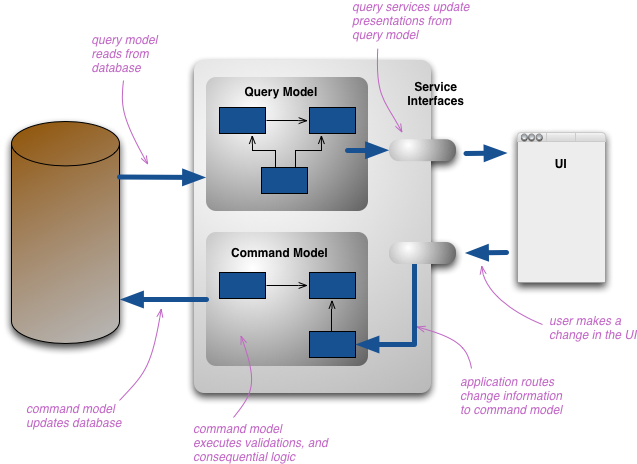
\includegraphics[width=\textwidth]{figures/cqrs.png}
    \caption{System split into query and command model following CQRS, taken from \cite{martin_fowler:cqrs}.}
    \label{fig:arch:cqrs}
\end{figure}

To take this even further, CQRS can also separate the system at the database level (see figure \ref{fig:arch:cqrs_es}), where the command model has its own database for writing data and the~query model has its own database that is optimized for reading (NoSQL database). All data changes (commands) then need to be propagated from the write database to the read database (i.e. by integration events and message queue). 

Typically, after an update command, the command model accesses its storage (also called the single source of truth) to ensure that the business rules are met, and then proceeds with the update. It is popular to use an \textbf{event sourcing} as the storage type, but it can also be used with a traditional relational database. The command model than publishes these changes to the message broker.

The query model is subscribed to data changing events from the message queue and updates its own database (i.e. MongoDB) as they arrive. To really improve performance and reduce read latency, it is necessary to make use of data redundancy in the NoSQL database to fit the query specifications, which likely implies complex updates to the NoSQL database.

This system leverages to maximum the ability of CQRS to use different technologies for each model, but comes with different sort of problems. The main downside of this approach is the more complex system with eventual consistency. Not every system is ideal for this approach and it may be beneficial to use simple CQRS and introduce \textbf{Cache-Aside pattern}\footnote{\url{https://learn.microsoft.com/en-us/azure/architecture/patterns/cache-aside}} to~reduce latency.

\begin{figure} [H]
    \centering
    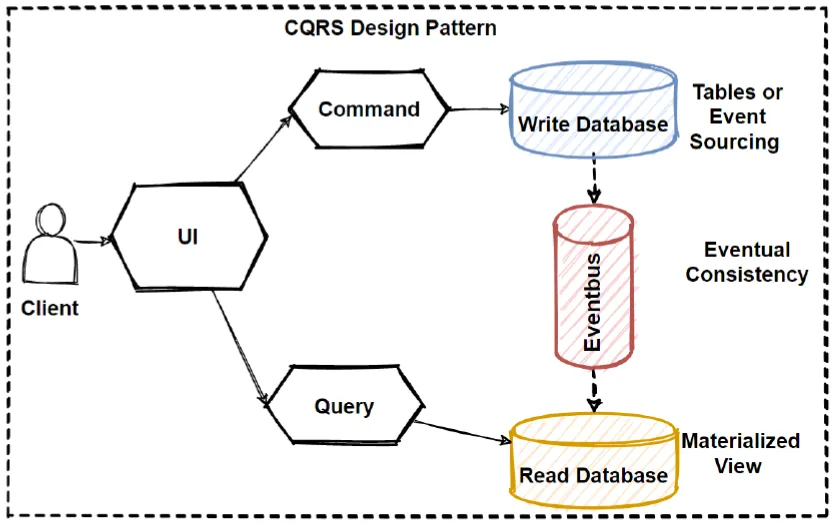
\includegraphics[width=\textwidth]{figures/cqrs-es.png}
    \caption{CQRS system modeled with split database tier and eventual consistency between databases, taken from \cite{mehmet_ozkaya:cqrs}.}
    \label{fig:arch:cqrs_es}
\end{figure}

\newpage
\subsection{Unit of Work}
\label{theory:unit_of_work}
According to the book Patterns of Enterprise Application Architecture \cite{martin_fowler:poeaa:unit_of_work} the Unit of Work:

\textit{"Maintains a list of objects affected by a business transaction and coordinates the writing out of changes and the resolution of concurrency problems."}

Essentially, instead of multiple SQL update requests, the unit of work merges all changes made to domain objects into a single transaction, thereby increasing performance, simplifying error handling and reducing the potential scope of unwanted side effects and bugs.

The unit of work is usually implemented into the ORM frameworks, but it might be beneficial to abstract the ORM away from the domain and application layers (Clean Architecture principles, see \ref{theory:clean_architecture}). The abstraction can be in the form of repositories (for~registering domain changes) and a custom unit of work interface/façade around the ORM for committing transactions.

\subsection{Transactional Outbox Pattern}
\label{theory:outbox}
The outbox pattern is a way to reliably publish asynchronous messages (e.g. send email), and is commonly used when publishing integration events or domain events in case of~domain with eventual consistency (for example with CQRS, see \ref{theory:CQRS}).

\subsubsection{Reliability problem}
The reliability problem in the context of publishing asynchronous messages can be demonstrated by a simple example of the requirement to send an email after a bank balance changed with concrete amount.

Sending emails must be asynchronous as the systems ability to send emails might be limited and the server response cannot be stalled, furthermore:

\begin{itemize}
    \item The email must be send only if the balance change is successful, that is, the transaction with saving the new balance completed successfully. Hence sending the email must be done outside of the application transaction.
    \item Email sending must be tracked so that if the server/application crashes right after a successful transaction and before the email is sent, after recovery the system can determine whether the email was sent or not and act accordingly.
\end{itemize}

\subsubsection{Outbox}
The solution to the reliability problem is to introduce an additional table into the database called outbox, to which the application stores records (outbox messages) indicating a desire to publish a message. The saving of outbox messages takes place within the application transaction, meaning that if other parts of the business logic (or event the outbox message storing itself) fail, and therefore transaction fails, the outbox message will not get persisted (and published).

The outbox message records contain information necessary for correct publishing, such as~the~message body (for example, a serialized integration event), timestamp, or whether the~message has already been published. 

The final part of the solution is a periodic job (e.g. every 10 seconds) responsible for~retrieving unpublished messages from outbox and trying to publish them. If publishing was successful, the outbox message is marked as published (or deleted right away). Failing to~publish results in a retry in the next job period.

\begin{figure} [H]
    \centering
    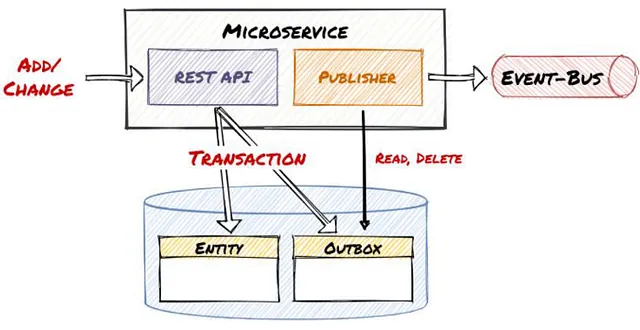
\includegraphics[width=0.8\textwidth]{figures/outbox.png}
    \caption{A diagram showcasing necessary parts and steps when utilizing the transactional outbox pattern, taken from \cite{mehmet_ozkaya:outbox}.}
    \label{fig:arch:outbox}
\end{figure}

Likewise, to reliably consume messages/events from message-broker/event bus, an inverse approach with \textbf{inbox} can be used.

The inbox and outbox patterns are commonly implemented in the communication libraries and frameworks (such as MassTransit\footnote{\url{https://masstransit.io/}}, NServiceBus\footnote{\url{https://particular.net/nservicebus}}, etc.), which then only need to be properly configured to access the database.

\chapter{Developing information system}
\label{chapter_dev}
This chapter delves into the developing process of a modular information system. It opens with a description of a demonstration application (section \ref{dev:demo}). 

Next, in section \ref{dev:analysis} the chapter covers the basic application analysis, including its use cases and analysis for the usage of CQRS and selected technologies.

It then continues with section \ref{dev:modeling} about modeling the domain according to the domain-driven design, including the application of strategy design (subdomains and bounded contexts) and tactical design (modeling aggregates).

This is followed by sections \ref{dev:clean_architecture} and \ref{dev:modular_monolith} covering the development of the Clean Architecture and Modular Monolith solutions, respectively, and their implementation details.

Section \ref{dev:frontend} deals with implementing a frontend application that effectively uses the backend solution regardless of the backend architecture  variant.

The chapter concludes with section \ref{dev:interesting}, describing interesting parts of~the~development of~modular information system solutions, such as enforcing architecture rules, and so on.

\section{Demonstration  application}
\label{dev:demo}
Team and event management application, with working title \textbf{TeamUp}, primarily focused on managing small sports teams.\footnote{Similar to application \url{https://tymuj.cz/}.}

In the application, the user can be part of a team as a regular team member, team coordinator or a team owner. In order to invite new users to the team or remove them, a member must be at least a team coordinator. There can be only one team owner, and a user can become one by creating a team or by being the target of ownership change. The team coordinator (as well as the team owner) creates team events, to which all team members respond whether they can attend or not. Only the team owner can assign roles. 

\subsubsection{Details}
\begin{itemize}
    \item Inviting is done via user's email regardless of the user's existence.
    \item Users can have a different nickname for each team they are member of.
    \item There must be business rules for maximum owned teams and maximum team capacity.
    \item Events can be distinguished by the event type.
    \item Members have several reply options to the team event -- member will not attend, member might attend, member will attend with delay, member will attend on time.
    \item Members can add a message to the reply to specify the reason behind their response.
\end{itemize}

\section{Application analysis}
\label{dev:analysis}
The application use case can be summarized using the use case diagram (see figure \ref{fig:dev_usecase}).

\begin{figure} [H]
    \centering
    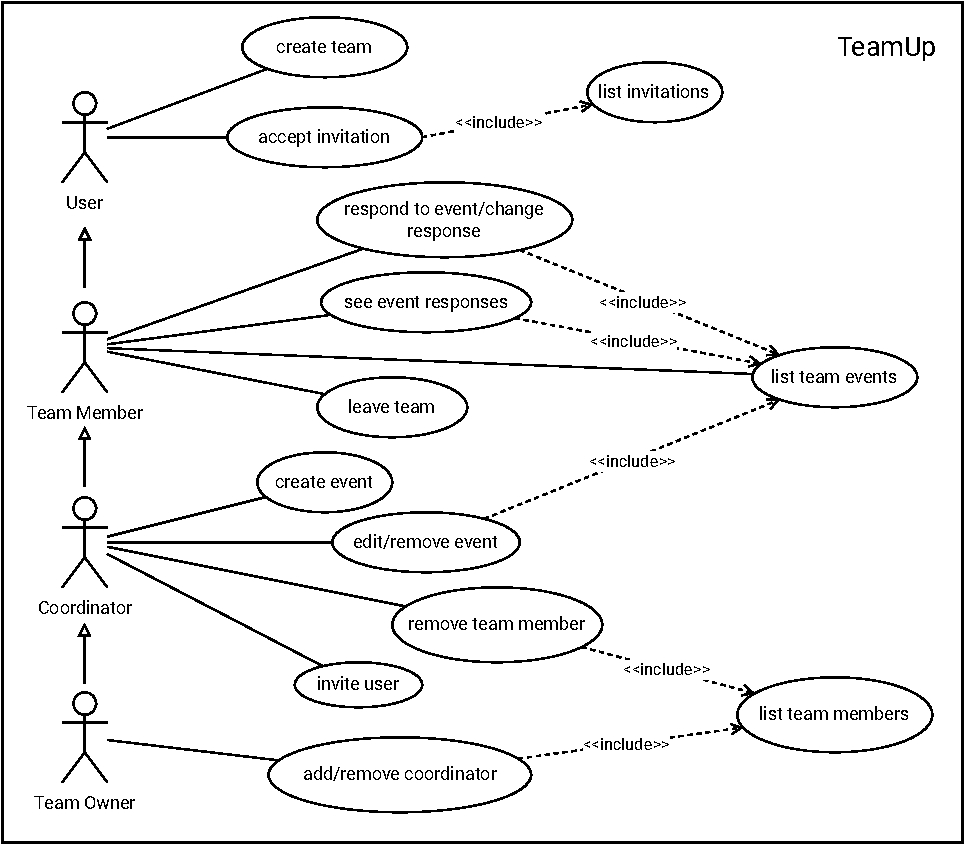
\includegraphics[width=1\textwidth]{figures/usecase.pdf}
    \caption{Use case diagram of the demonstration application.}
    \label{fig:dev_usecase}
\end{figure}

The use case diagram can serve as a basis for identifying basic commands and queries in~the~context of CQRS:

\textbf{Commands}: create/update/remove team, accept invitation, create response, update response, create/update/remove event type, create/(update)/remove event, invite user/remove invitation, remove team member, assign role.

Updating an event may not be a desirable feature because when changing, for example, the start time of an event, members may need to change their responses, leading to a hard-to-solve business problem of how to react in such situation (clear all responses/leave all responses/sophisticated solution).

\textbf{Queries}: get team (including team members and event types), get events (including number of responses of each type), get event (including all responses), get user's invitations, get team invitations, get user's teams.

Based on the way the application works, it can be assumed that most of the demands will target the queries \textbf{get events} and \textbf{get event} and the \textbf{create response} command, as these are the application's daily use cases. There may be other frequently called queries, such as~\textbf{get team}, but these change relatively infrequently and may be cached.

\subsection{General technologies}
\begin{itemize}
    \item Platform: \textbf{dotnet} platform with the \textbf{C\#} language is considered an elite platform for~enterprise-wide information systems. In addition to quality documentation, Microsoft provides a variety of free eBooks\footnote{\url{https://dotnet.microsoft.com/en-us/learn/dotnet/architecture-guides}} for building systems on the dotnet platform.
    
    \item Backend RESTful API: \textbf{ASP.NET Core} is an open source cross-platform framework maintained by Microsoft for building web applications and services.
    
    \item Database: \textbf{PostgreSQL}\footnote{\url{https://www.postgresql.org/}} (postgres) is a free and open-source relational database management system, and in my experience it spins up instance in docker much faster then the SQL Server (traditional choice for dotnet), resulting in faster integration and E2E testing, and thus making it my choice.
    
    \item Data access: \textbf{Entity Framework Core} (EF Core) is widely used ORM by Microsoft with support for code-first modeling workflow and database migrations.
    
    \item Background service scheduling: \textbf{Quartz.NET}\footnote{\url{https://www.quartz-scheduler.net/}} is a popular open-source job scheduling system targeting dotnet.
\end{itemize}

\section{Modeling domain}
\label{dev:modeling}
When using DDD, the first step is to apply strategy design, which is mainly identifying subdomains and bounded contexts. Additionally, denoting shared kernels for multi-bounded context systems, and so on.

The next step is to apply tactical design, which consists of modeling the domain for a given bounded context and identifying  aggregates and value objects. 

Further modeling is done in the code using patterns such as domain events, domain services, etc. (described in section \ref{ddd:tactical_design}), in conjunction with continuous refactoring.

\subsection{Identifying subdomains and bounded contexts}
The core business logic of the system is team management, which involves managing team members and their roles + managing team events and responding to events. This could be viewed as one big team management subdomain, but I am leaning towards splitting it into 2 core subdomains -- \textbf{Teams} subdomain and \textbf{Events} subdomain (see \ref{ddd:strategy_design}), which decouples parts of the system and better visualizes the integration relationships between individual subdomains.

Inviting users to the team is not the core of the application, as no user would start using the application because of this functionality, indicating it as a supporting subdomain.

The application has to provide basic user account functions (registration, login, etc.), this is a common problem and the system does not need some application specific features, based on that this area appears as a generic subdomain -- in the diagram \ref{fig:teamup-strategy-design} called \textbf{User Access} subdomain.

\begin{figure} [H]
    \centering
    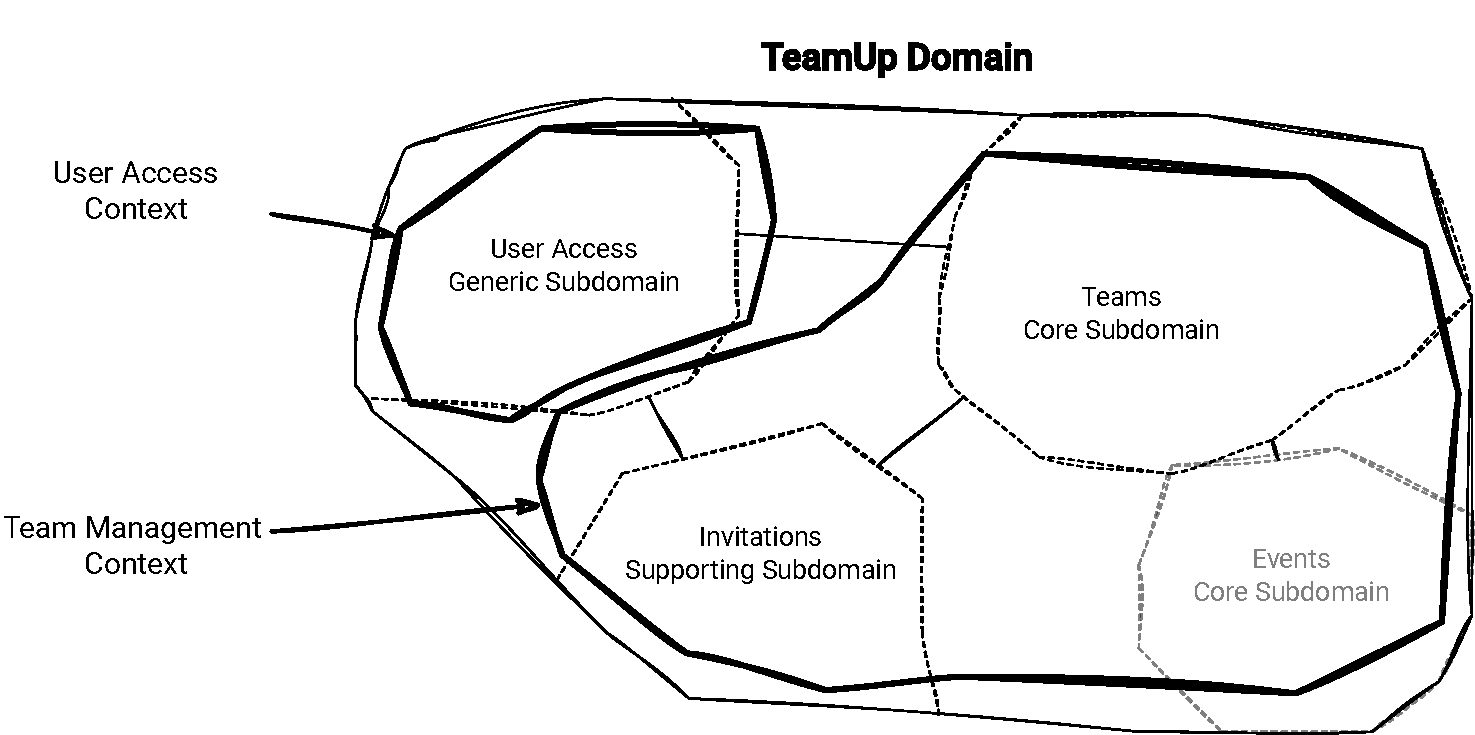
\includegraphics[width=\textwidth]{figures/teamup-strategy-design.pdf}
    \caption{System domain decomposed to subdomains and bounded contexts.}
    \label{fig:teamup-strategy-design}
\end{figure}

User access has its own bounded context as it should be managed by an existing solution\footnote{This would be true for a real-world application, however, the purpose of this thesis is not the integration of an identity server, so the solutions will implement a simple JWT authentication only with basic functions required by the business (register, login, delete and activate account).} and will not need any insight into the core/supporting domains of the application.

The rest of the subdomains can be modelled as a single bounded context as the domains have the same view at the system entities (the team is the same from both the invitation and the event perspective). There is the overlap with user access subdomain as the team management context has to have some reference to users (i.e. in form of an id) and occasionally access users properties to implement application use cases (inviting via email and so on).

\subsection{Domain model}
Typically each bounded context would have its own domain model, however, since the user access context has only one entity from which most of the properties are used in the team management context, it would be counterproductive to treat them as separate contexts (may be different for modular monolith architecture as it separates system into modules).
\begin{figure} [H]
    \centering
    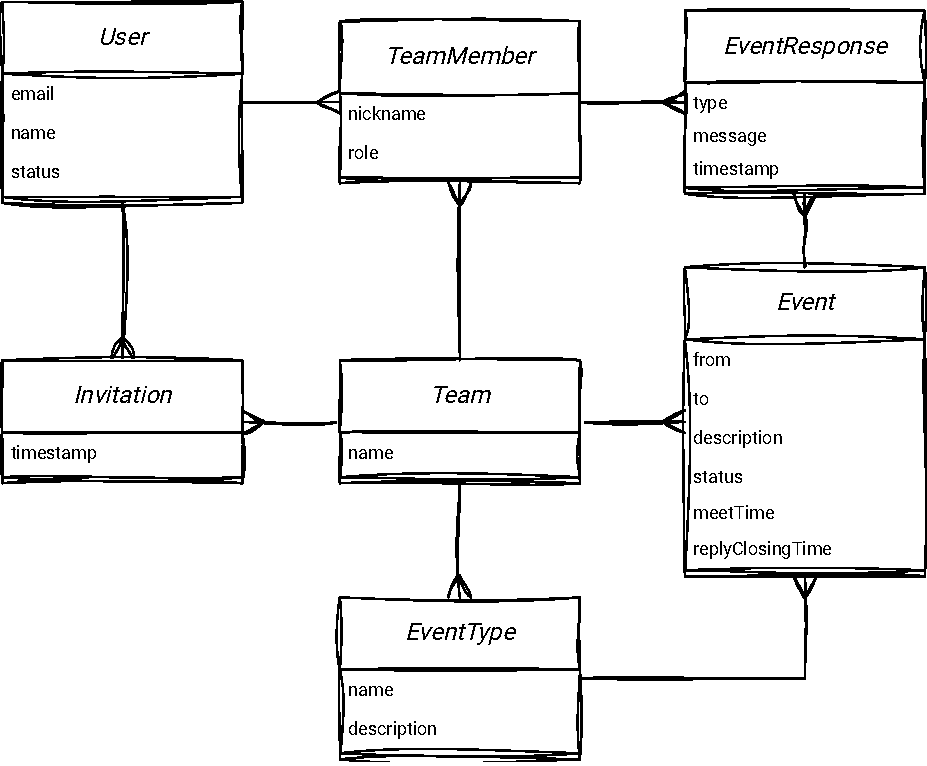
\includegraphics[width=1\textwidth]{figures/domain-0.pdf}
    \caption{The initial domain model of the modeled system, where identifiers are PK for~all entities and all relationships are 1:N, the model serves as the starting point and does not specify data types, visibility or methods implementing the business logic. It is mainly intended to showcase relationships and properties required by the business.}
    \label{fig:dev_domains}
\end{figure}

\subsection{Modeling aggregates}
A common approach to modeling aggregates is to start with an initial domain and mark all entities as the aggregate roots (see figure \ref{fig:domain_aggregates_1}), then gradually try to merge the aggregates together or mark them as a final aggregate. 

Before modeling aggregates, it is necessary to identify the value objects, for instance, the \texttt{EventResponse} containing the response type and message can be extracted into an \texttt{EventReply} value object to improve object manipulation and enforce business rules. 

Theoretically, the \texttt{EventType} could be a value object as the team already contains event references and it is defined only by name and description, however, this would cause problems when updating the event type name since value objects are immutable (see \ref{ddd:entities_and_value_objects}). 
 
\begin{figure} [H]
    \centering
    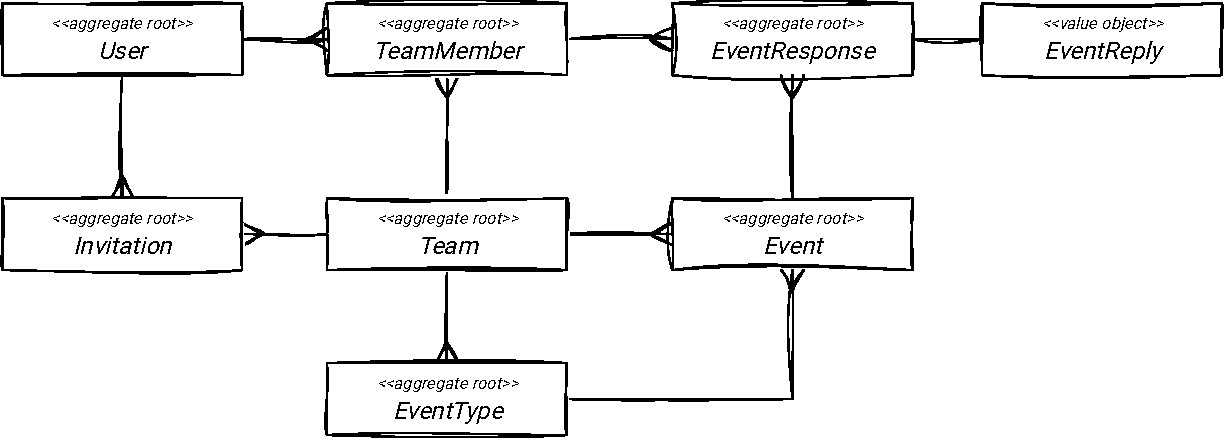
\includegraphics[width=\textwidth]{figures/domain-aggregates-1.pdf}
    \caption{Diagram representing initial point for modeling aggregates with each entity serving as an aggregate root. Diagram contains unresolved relationships as DDD states that aggregates cannot reference each other directly.}
    \label{fig:domain_aggregates_1}
\end{figure}

Merging \texttt{EventResponse} into the \textbf{event aggregate} makes sense as the response is directly associated with the event and the user must interact with the event to create/update the~response. The \text{Event} serves as an interface for event response manipulation and takes advantage of the \texttt{EventReply} value object to set the response directly from its interface.

Similarly, the \texttt{TeamMember} is an ideal candidate for merging into the \textbf{team aggregate} since the \texttt{Team} has all the necessary data for validating actions affecting team members (assigning roles, removing members, and so on).

The \texttt{User} has no interaction with other entities and thus is a good candidate for aggregate root. To some extent, it might make sense to manipulate invitations through the \texttt{User}, however, the same applies to the invitation-team relationship. Moreover, in the strategy design (figure \ref{fig:teamup-strategy-design}), the invitations are modeled as a separate subdomain, therefore it is logical to leave \texttt{Invitation} as its own aggregate and handle invitations through a domain service.

\begin{figure} [H]
    \centering
    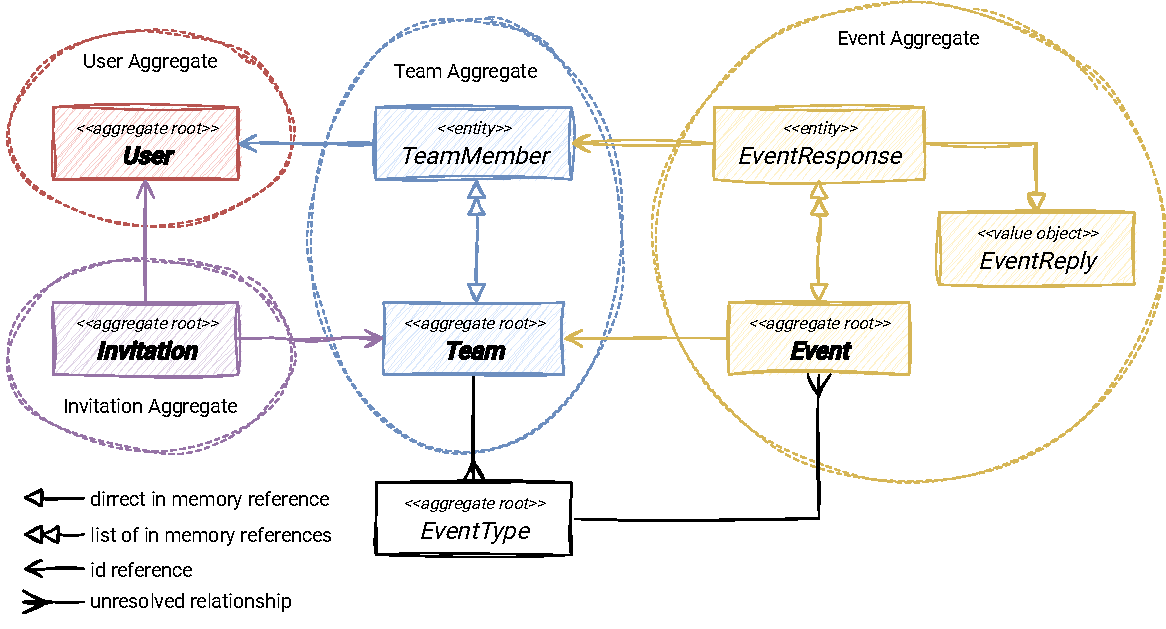
\includegraphics[width=\textwidth]{figures/domain-aggregates-2.pdf}
    \caption{Domain model with partially modeled aggregates.}
    \label{fig:domain_aggregates_2}
\end{figure}

The \texttt{EventType} is tightly associated with the \texttt{Event}, however, all the manipulation needs to go trough the \textbf{team aggregate} so that the team aggregate root can authorize changes based on the initiator role. Furthermore, \texttt{EventType} references multiple events, so merging it into the event aggregate does not really make sense.

\begin{figure} [H]
    \centering
    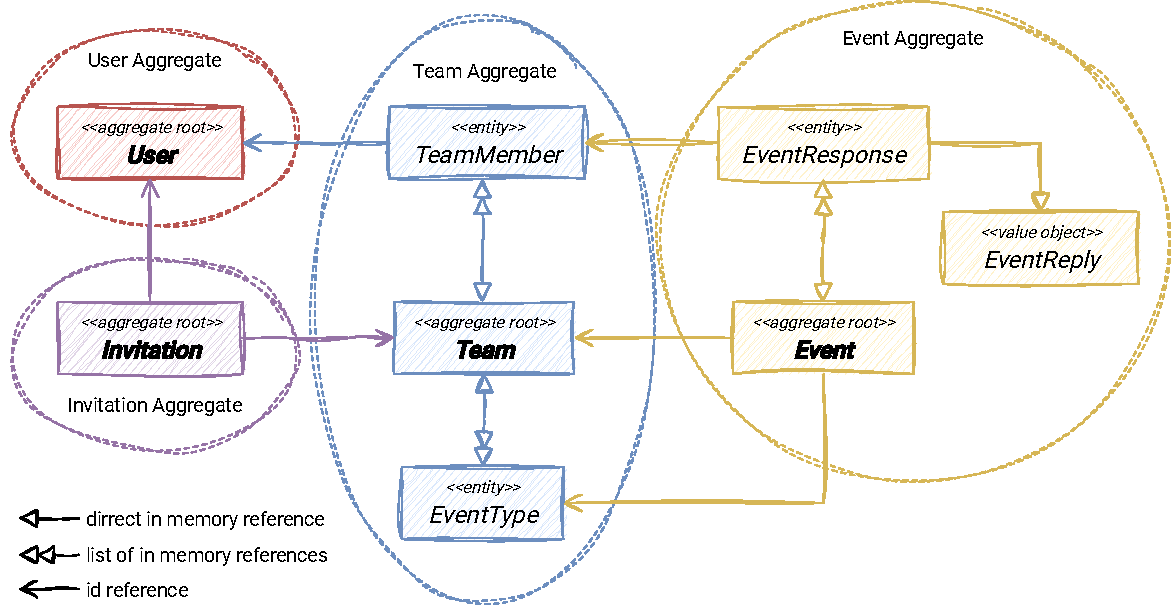
\includegraphics[width=\textwidth]{figures/domain-aggregates-3.pdf}
    \caption{Diagram of final domain model designed with DDD. The diagram shows 3 apparent references from the event aggregate to the team aggregate. Although this might indicate candidates for merging, the resulting aggregate would be far too large. Furthermore, the domain services will resolve any logic requiring both aggregates.}
    \label{fig:domain_aggregates_3}
\end{figure}

\section{Clean Architecture solution}
\label{dev:clean_architecture}
The entire Clean Architecture solution is available online as a repository on GitHub:

\url{https://github.com/skrasekmichael/CleanArchitecture}

\subsection{System Design}
\label{dev:ca:deisgn}
The system takes advantage of the CQRS with a single database:
\begin{itemize}
    \item Query Part -- applies simple authorization validations in handlers and communicates with the~database through a query context to enable more performant querying.
    \item Command Part -- utilizes Domain-Driven Design and its patterns to enforce complex business rules and validations (factories, aggregates and domain services) and ensures system consistency (domain events).
\end{itemize}

\begin{figure} [H]
    \centering
    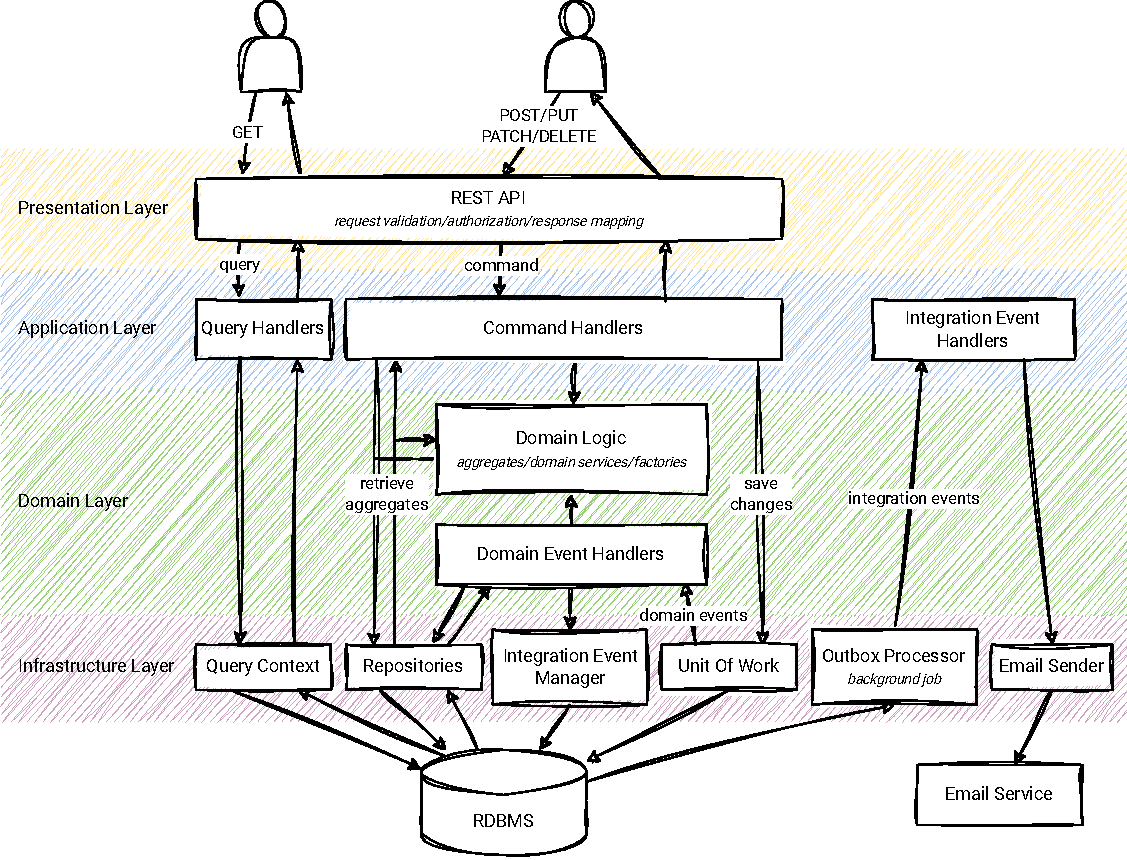
\includegraphics[width=\textwidth]{figures/ca-design.pdf}
    \caption{Diagram showcasing the flow through the Clean Architecture solution and some of its components. The infrastructure layer may look like innermost layer, however, the~application and domain layers do not depend on the~infrastructure layer at compile time, but rather use interfaces whose implementation is provided by the infrastructure layer via~dependency injection at runtime. The diagram also illustrates the apparent complexity difference in the implementation of the query part (2 components) and the command part.}
    \label{fig:ca_design}
\end{figure}

\subsection{Implementing solution}
Project structure: \vspace{6pt}

\dirtree{%
.1 TeamUp/\DTcomment{Clean Architecture repository}.
.2 src/.
.3 TeamUp.Common/\DTcomment{common types, abstractions and extensions}.
.3 TeamUp.Contracts/\DTcomment{API contracts and validators}.
.3 TeamUp.Domain/\DTcomment{domain model according to DDD}.
.3 TeamUp.Application/\DTcomment{commands and queries and their handlers}.
.3 TeamUp.Infrastructure/\DTcomment{EF Core configurations, migrations etc.}.
.3 TeamUp.Api/\DTcomment{ASP.NET Core RESTful API}.
.2 tests/.
.2 TeamUp.sln.
.2 \dots.
}

The \texttt{src} directory contains individual layers regarding the Clean Architecture with 2 additional layers (\texttt{Common} and \texttt{Contracts}).

The \texttt{tests} directory contains all aplication tests, including integration/E2E tests (see section \ref{dev:integration_testing}), architecture tests (section \ref{dev:arch_testing}), and so on.

\subsection{Common Layer}
The common layer contains common abstractions such as \texttt{IDateTimeProvider}, common types (e.g. exceptions/errors) and extension methods. 
 
The purpose of this layer, similarly to so called \textit{interface layer}, is to provide the necessary abstractions that can be used in other layers. Implementations of these abstractions reside in other layers (mainly in the infrastructure layer).

The common layer is not dependent on any other layer, and the only dependency is on~the~RailwayResult package (see section \ref{interesting:rp_rop} about the result pattern), providing contracts and extension methods for the entire system.

\subsection{Contract Layer}
The contract layer contains all the contracts required for calling the API, including responses, enums, strongly typed ids, requests and their validators. The layer also contains constants used for validating and preparing API requests.

The contract layer could be reused by other presentation layers (MVC backend, SPA, mobile app, 3rd party services, etc.) as a shared dependency without the need to redefining types.

The \textbf{FluentValidation}\footnote{\url{https://github.com/FluentValidation/FluentValidation}} package is used to validate requests by creating a validation class for each request and creating rules for request properties using the fluent API. The main advantage of the FluentValidation library is the ease of validation for more complex rules as showcased in figure \ref{fig:validator}.

\begin{figure} [H]
    \centering
    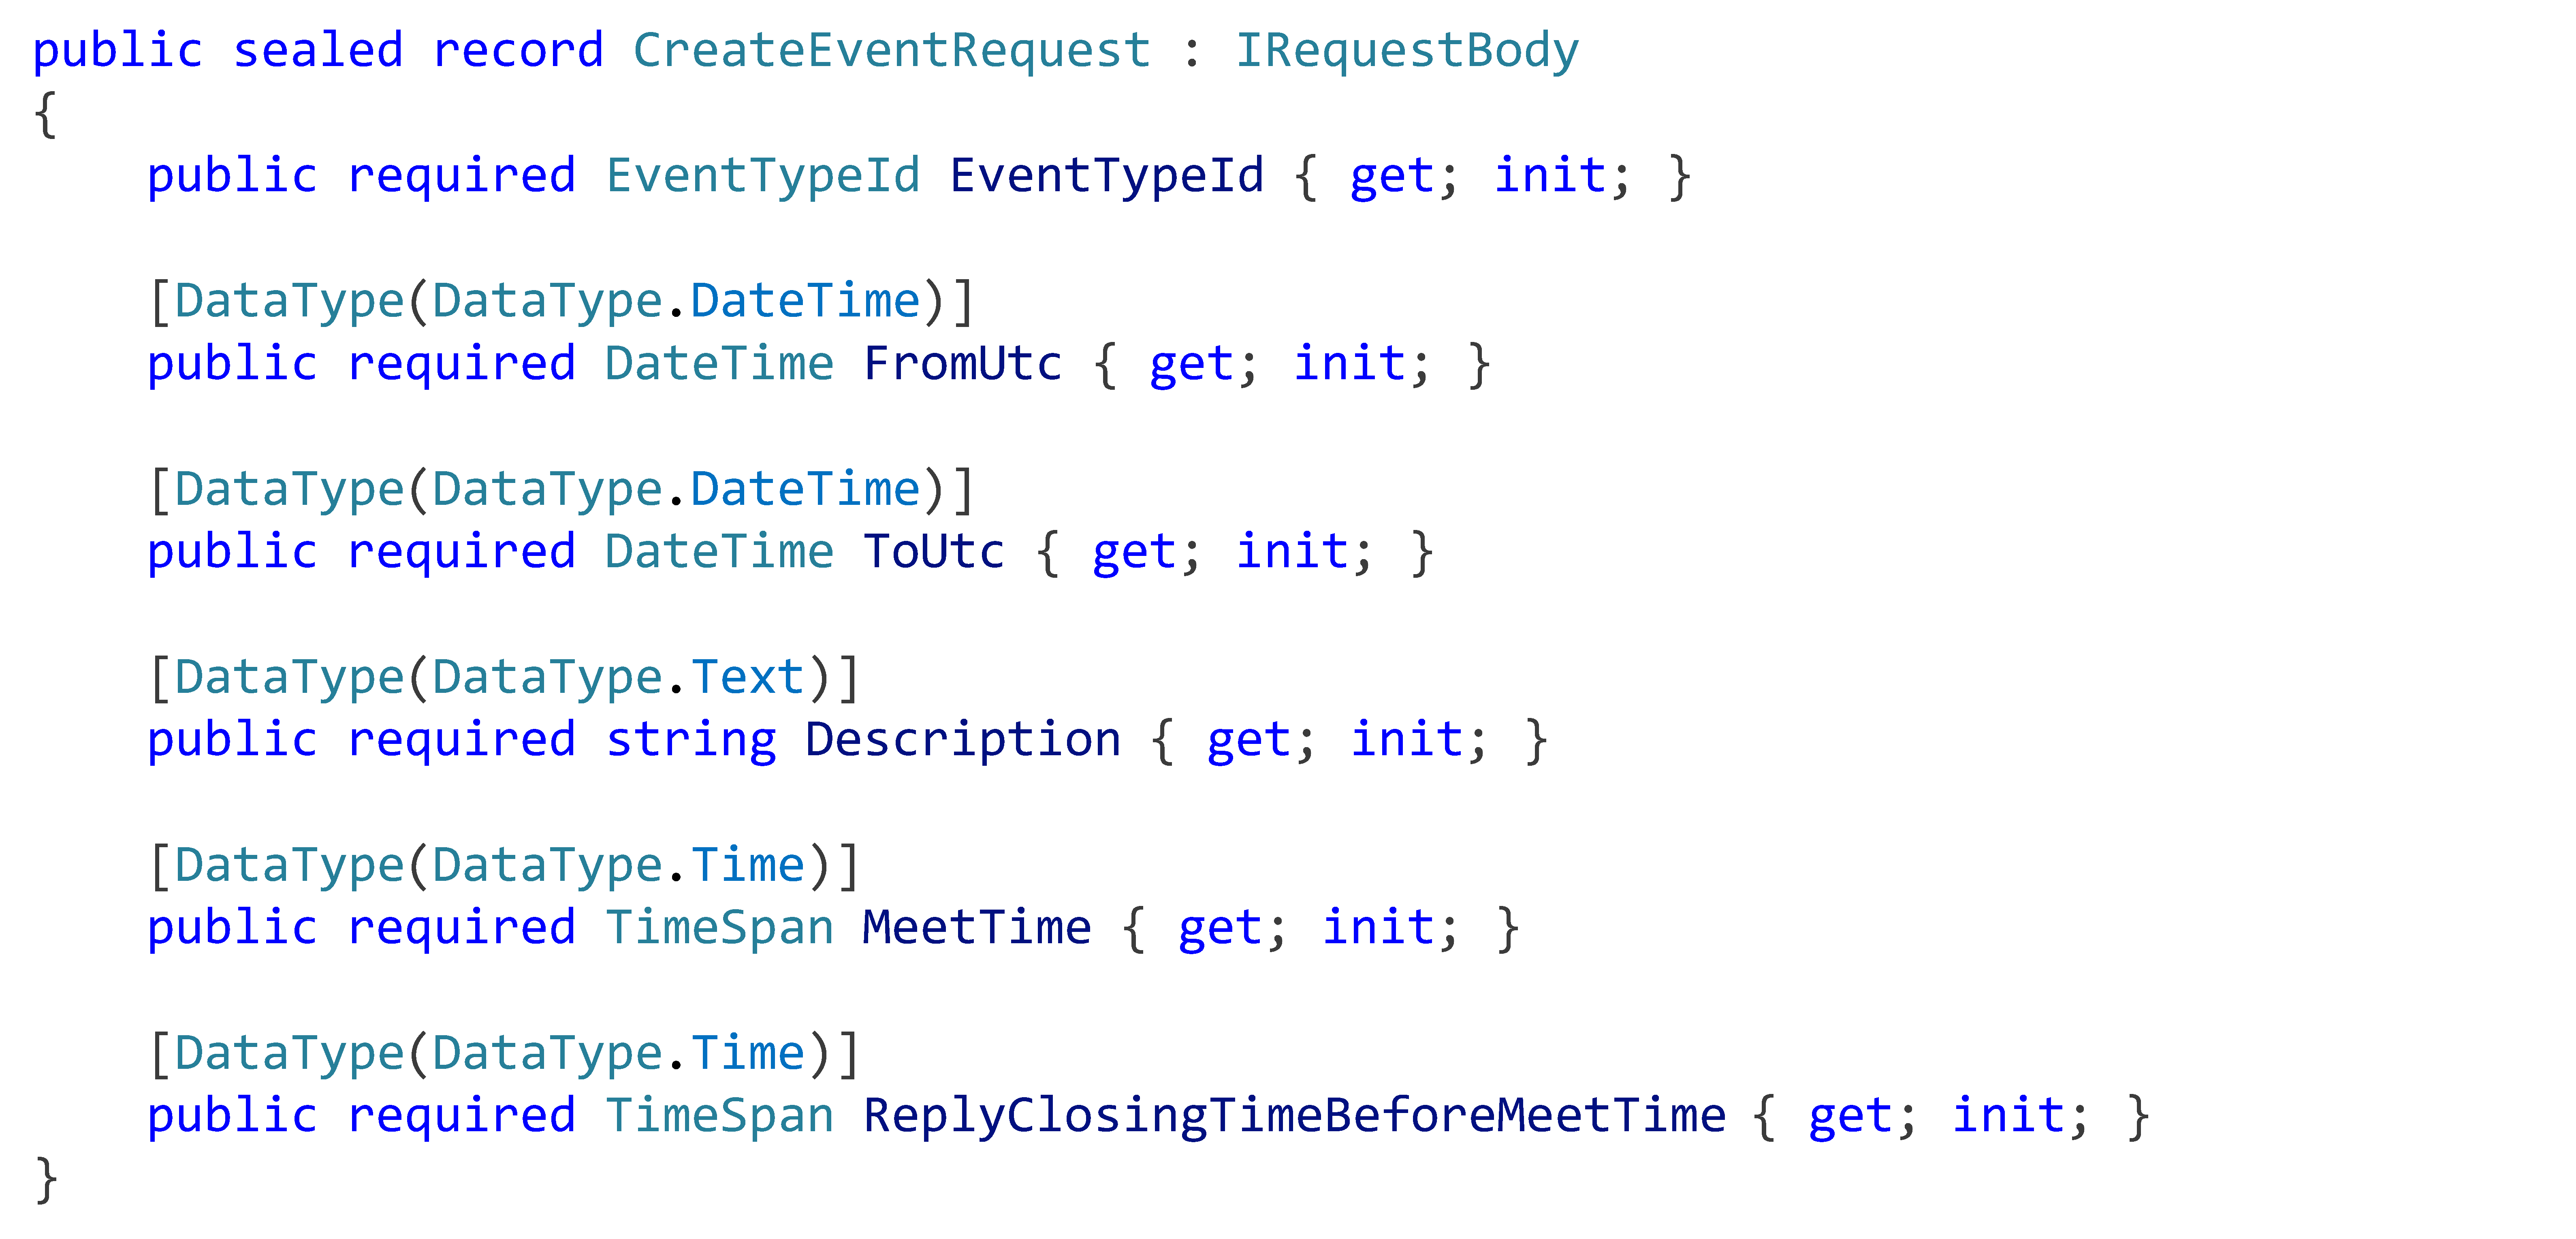
\includegraphics[width=\textwidth]{figures/request.pdf}
    \caption{Code sample of request (body) for creating an event. Properties are annotated with meta informations that could be used by templating engines from other presentation layers. Note that the \texttt{EventTypeId} property is defined as a strongly typed id, same as all other idefntifiers in the solution.}
    \label{fig:request}
\end{figure}

\begin{figure} [H]
    \centering
    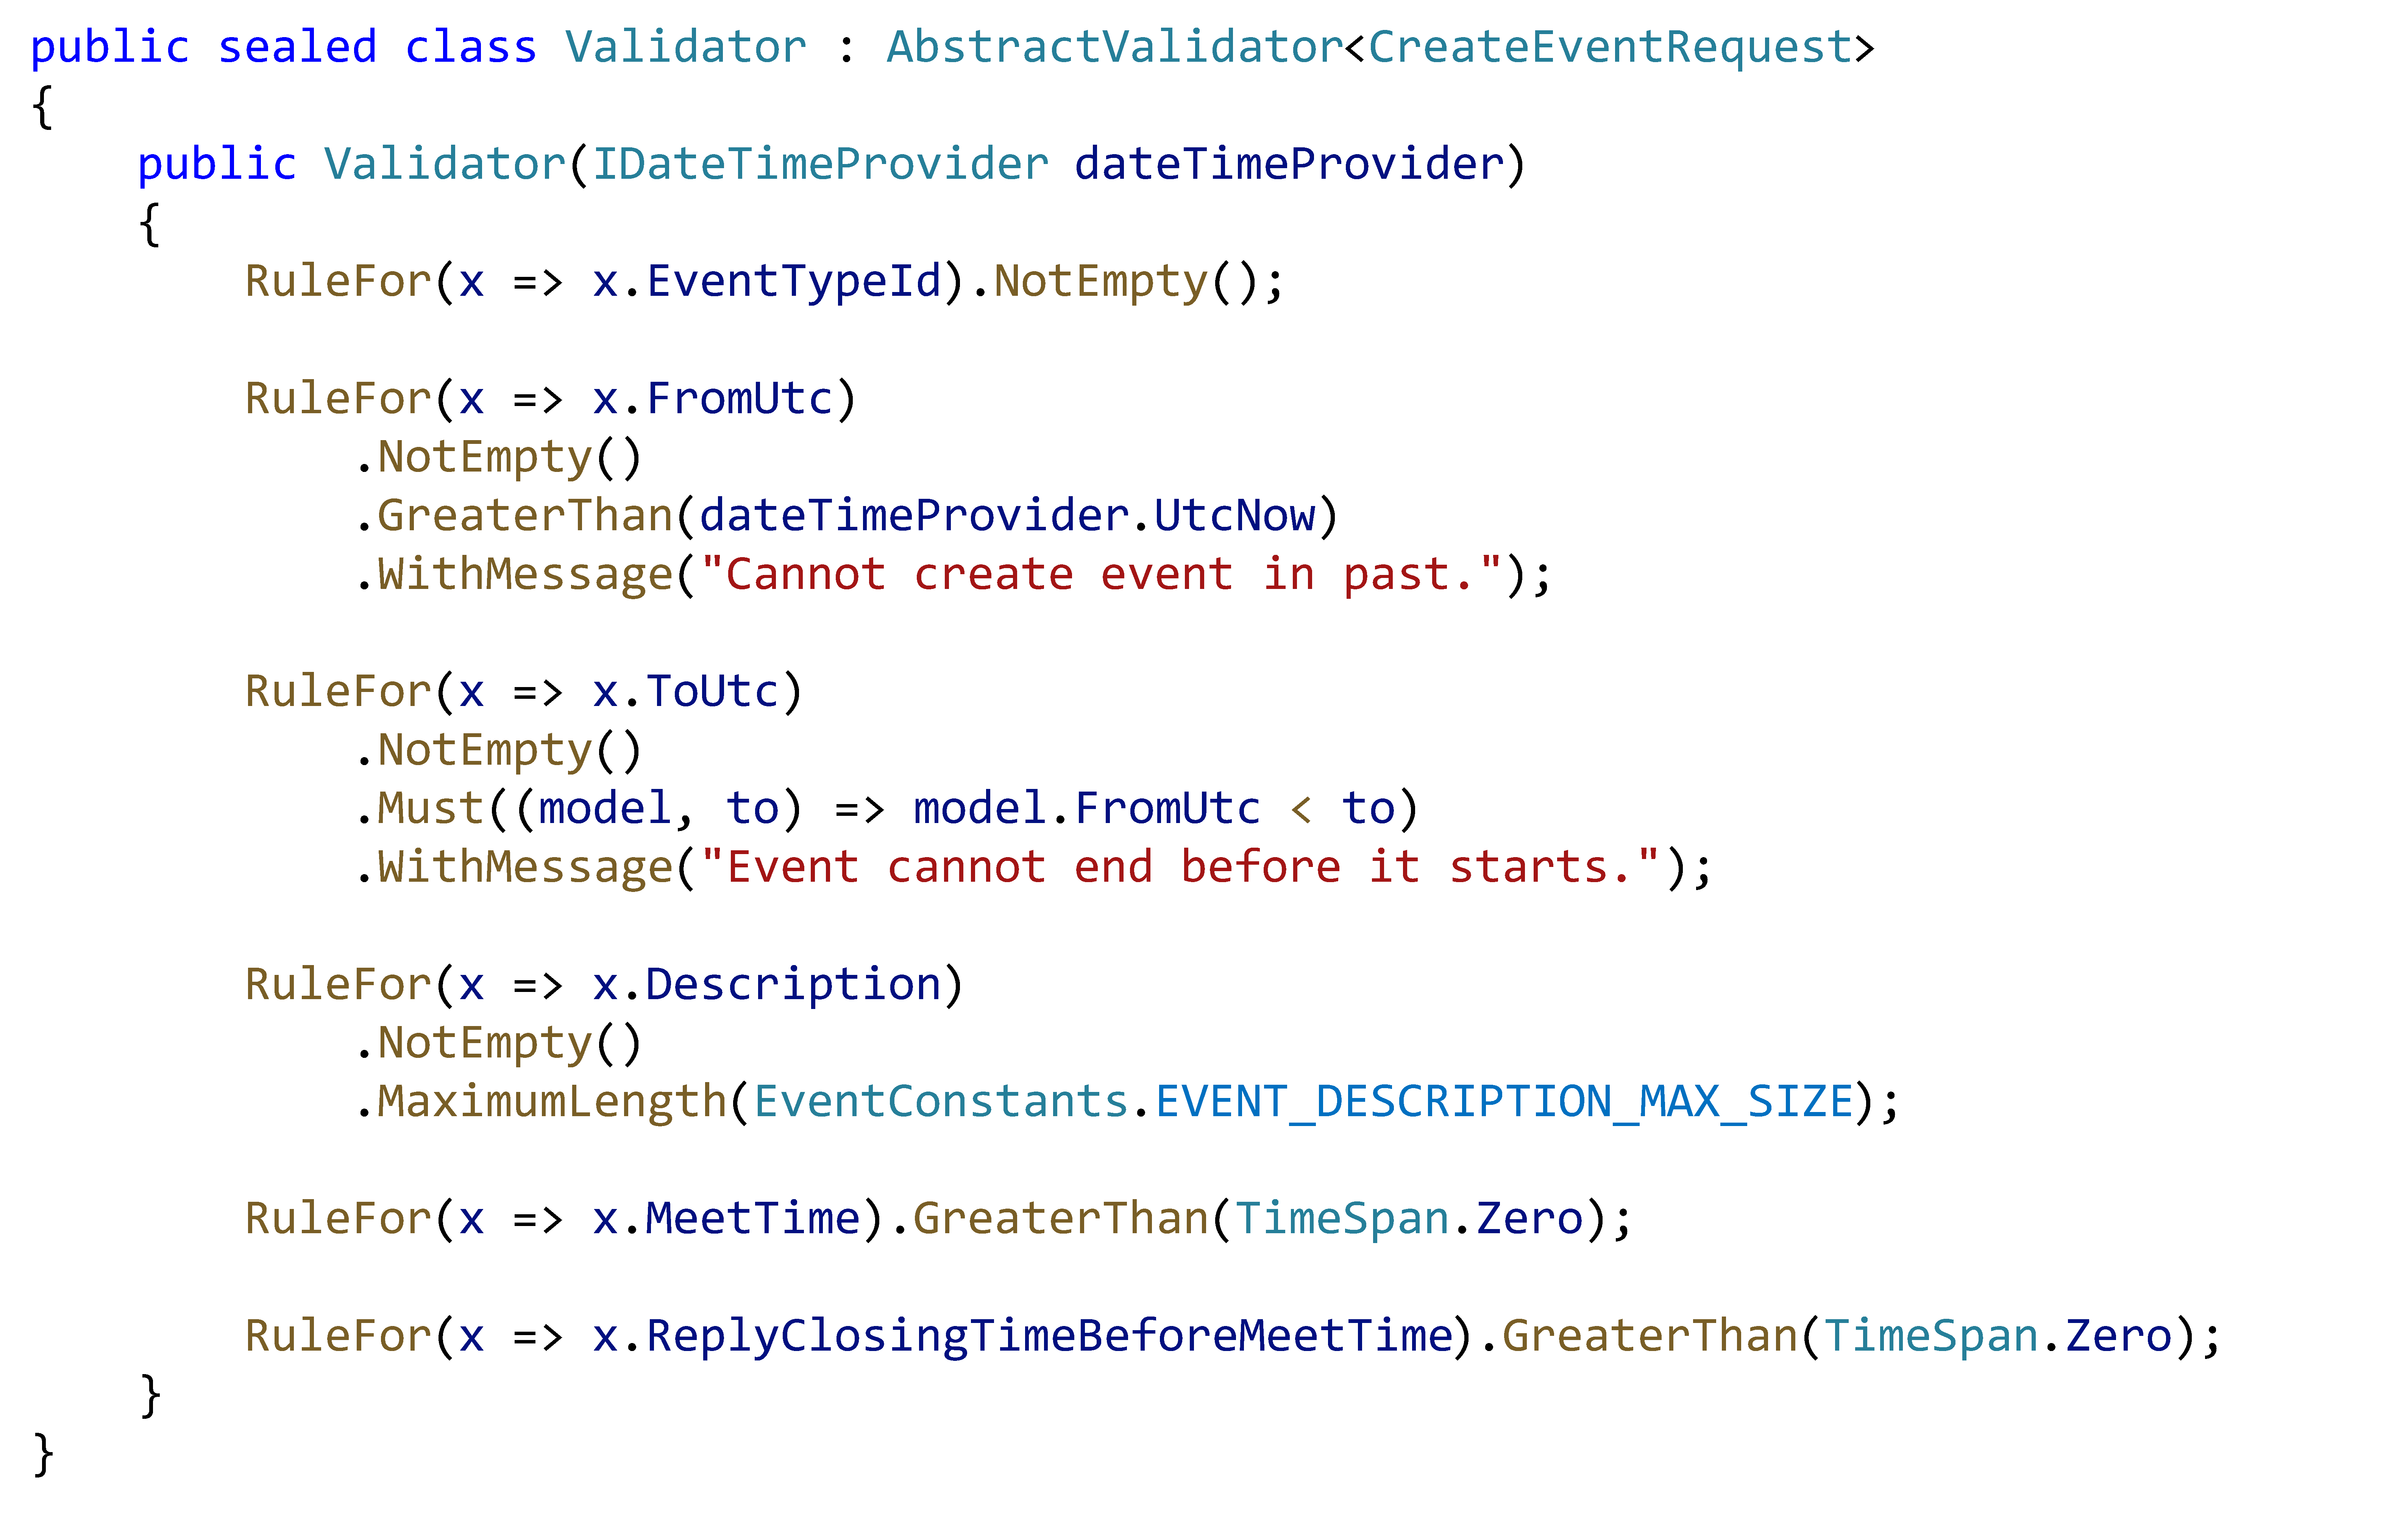
\includegraphics[width=\textwidth]{figures/validator.pdf}
    \caption{Code sample of a validator for \texttt{CreateEventRequest} (figure \ref{fig:request}) with more complex rules, working with \texttt{DateTimeProvider} or the rule of the \texttt{ToUtc} property dependent on~the~\texttt{FromUtc} property, which would be complicated to implement using the default annotation-based validation build in ASP.NET Core.}
    \label{fig:validator}
\end{figure}

\subsection{Domain Layer}
The domain layer contains domain-specific logic, that is:
\begin{itemize}
    \item Aggregates -- the \textbf{aggregate root entity} and additional nested entities and value objects for each aggregate.
    \item Aggregate specifics (grouped together with aggregates) -- factories, \textbf{domain events}, integration events and a \textbf{repository} interface that is used in other services (factories, event handlers, domain services, and command handlers). Additional possible aggregate specifics may include logic (extension methods) over enum types and static classes with defined business rules and errors.
    \item \textbf{Event Handlers} to synchronize and enforce a consistent state across aggregates (preferred method) and potentially to publish integration events.
    \item \textbf{Domain Services} with logic involving multiple aggregates and the necessity of data from other aggregates for immediate business rules validation.
    \item Abstractions for domain objects, i.e. for entities, domain events, event handlers, \dots
\end{itemize}

Detailed structure: \vspace{6pt}
\dirtree{%
.1 TeamUp.Domain/\DTcomment{domain layer}.
.2 Abstractions/\DTcomment{domain objects abstractions (aggregate root, entity \dots)}.
.2 Aggregates/.
.3 Invitations/\DTcomment{domain objects of the invitation aggregate}.
.3 Users/\DTcomment{domain objects of the user aggregate}.
.3 Events/.
.4 DomainEvents/\DTcomment{events published by the event aggregate}.
.4 Event.cs\DTcomment{aggregate root}.
.4 EventResponse.cs\DTcomment{nested entity}.
.4 EventReply.cs\DTcomment{value object}.
.4 EventStatusExtensions.cs\DTcomment{added logic for \texttt{EventStatus} enum}.
.4 EventErrors.cs\DTcomment{errors returned by the event aggregate}.
.4 IEventRepository.cs\DTcomment{repository definition for working with events}.
.3 Teams/.
.4 DomainEvents/\DTcomment{events published by the team aggregate}.
.4 Team.cs\DTcomment{aggregate root}.
.4 TeamMember.cs\DTcomment{nested entity}.
.4 EventType.cs\DTcomment{nested entity}.
.4 TeamRoleExtensions.cs\DTcomment{added logic for \texttt{TeamRole} enum}.
.4 TeamErrors.cs\DTcomment{errors returned by the tean aggregate}.
.4 TeamRules.cs\DTcomment{business rules of the team aggregate}.
.4 ITeamRepository.cs\DTcomment{repository definition for working with teams}.
.2 DomainServices/\DTcomment{domain services}.
.2 EventHandlers/\DTcomment{domain event handlers}.
.2 ServiceCollectionExtensions.cs\DTcomment{methods for registering layer to DI}.
.2 TeamUp.Domain.csproj\DTcomment{assembly file}.
}

\subsubsection{Domain Events}
Domain events are meant to propagate changes to other parts of the domain (mainly aggregates) and therefore enforce necessary actions to bring the domain into consistent state.

Some of the logic performed by the domain event handlers could be solved by database triggers, however, that would split up the business logic and pile up additional complexity.

Traditionally, domain events are not published/handled immediately, but rather gathered and handled at the end of a transaction (see more in section \ref{dev:ca:infra}).

\begin{figure} [H]
    \centering
    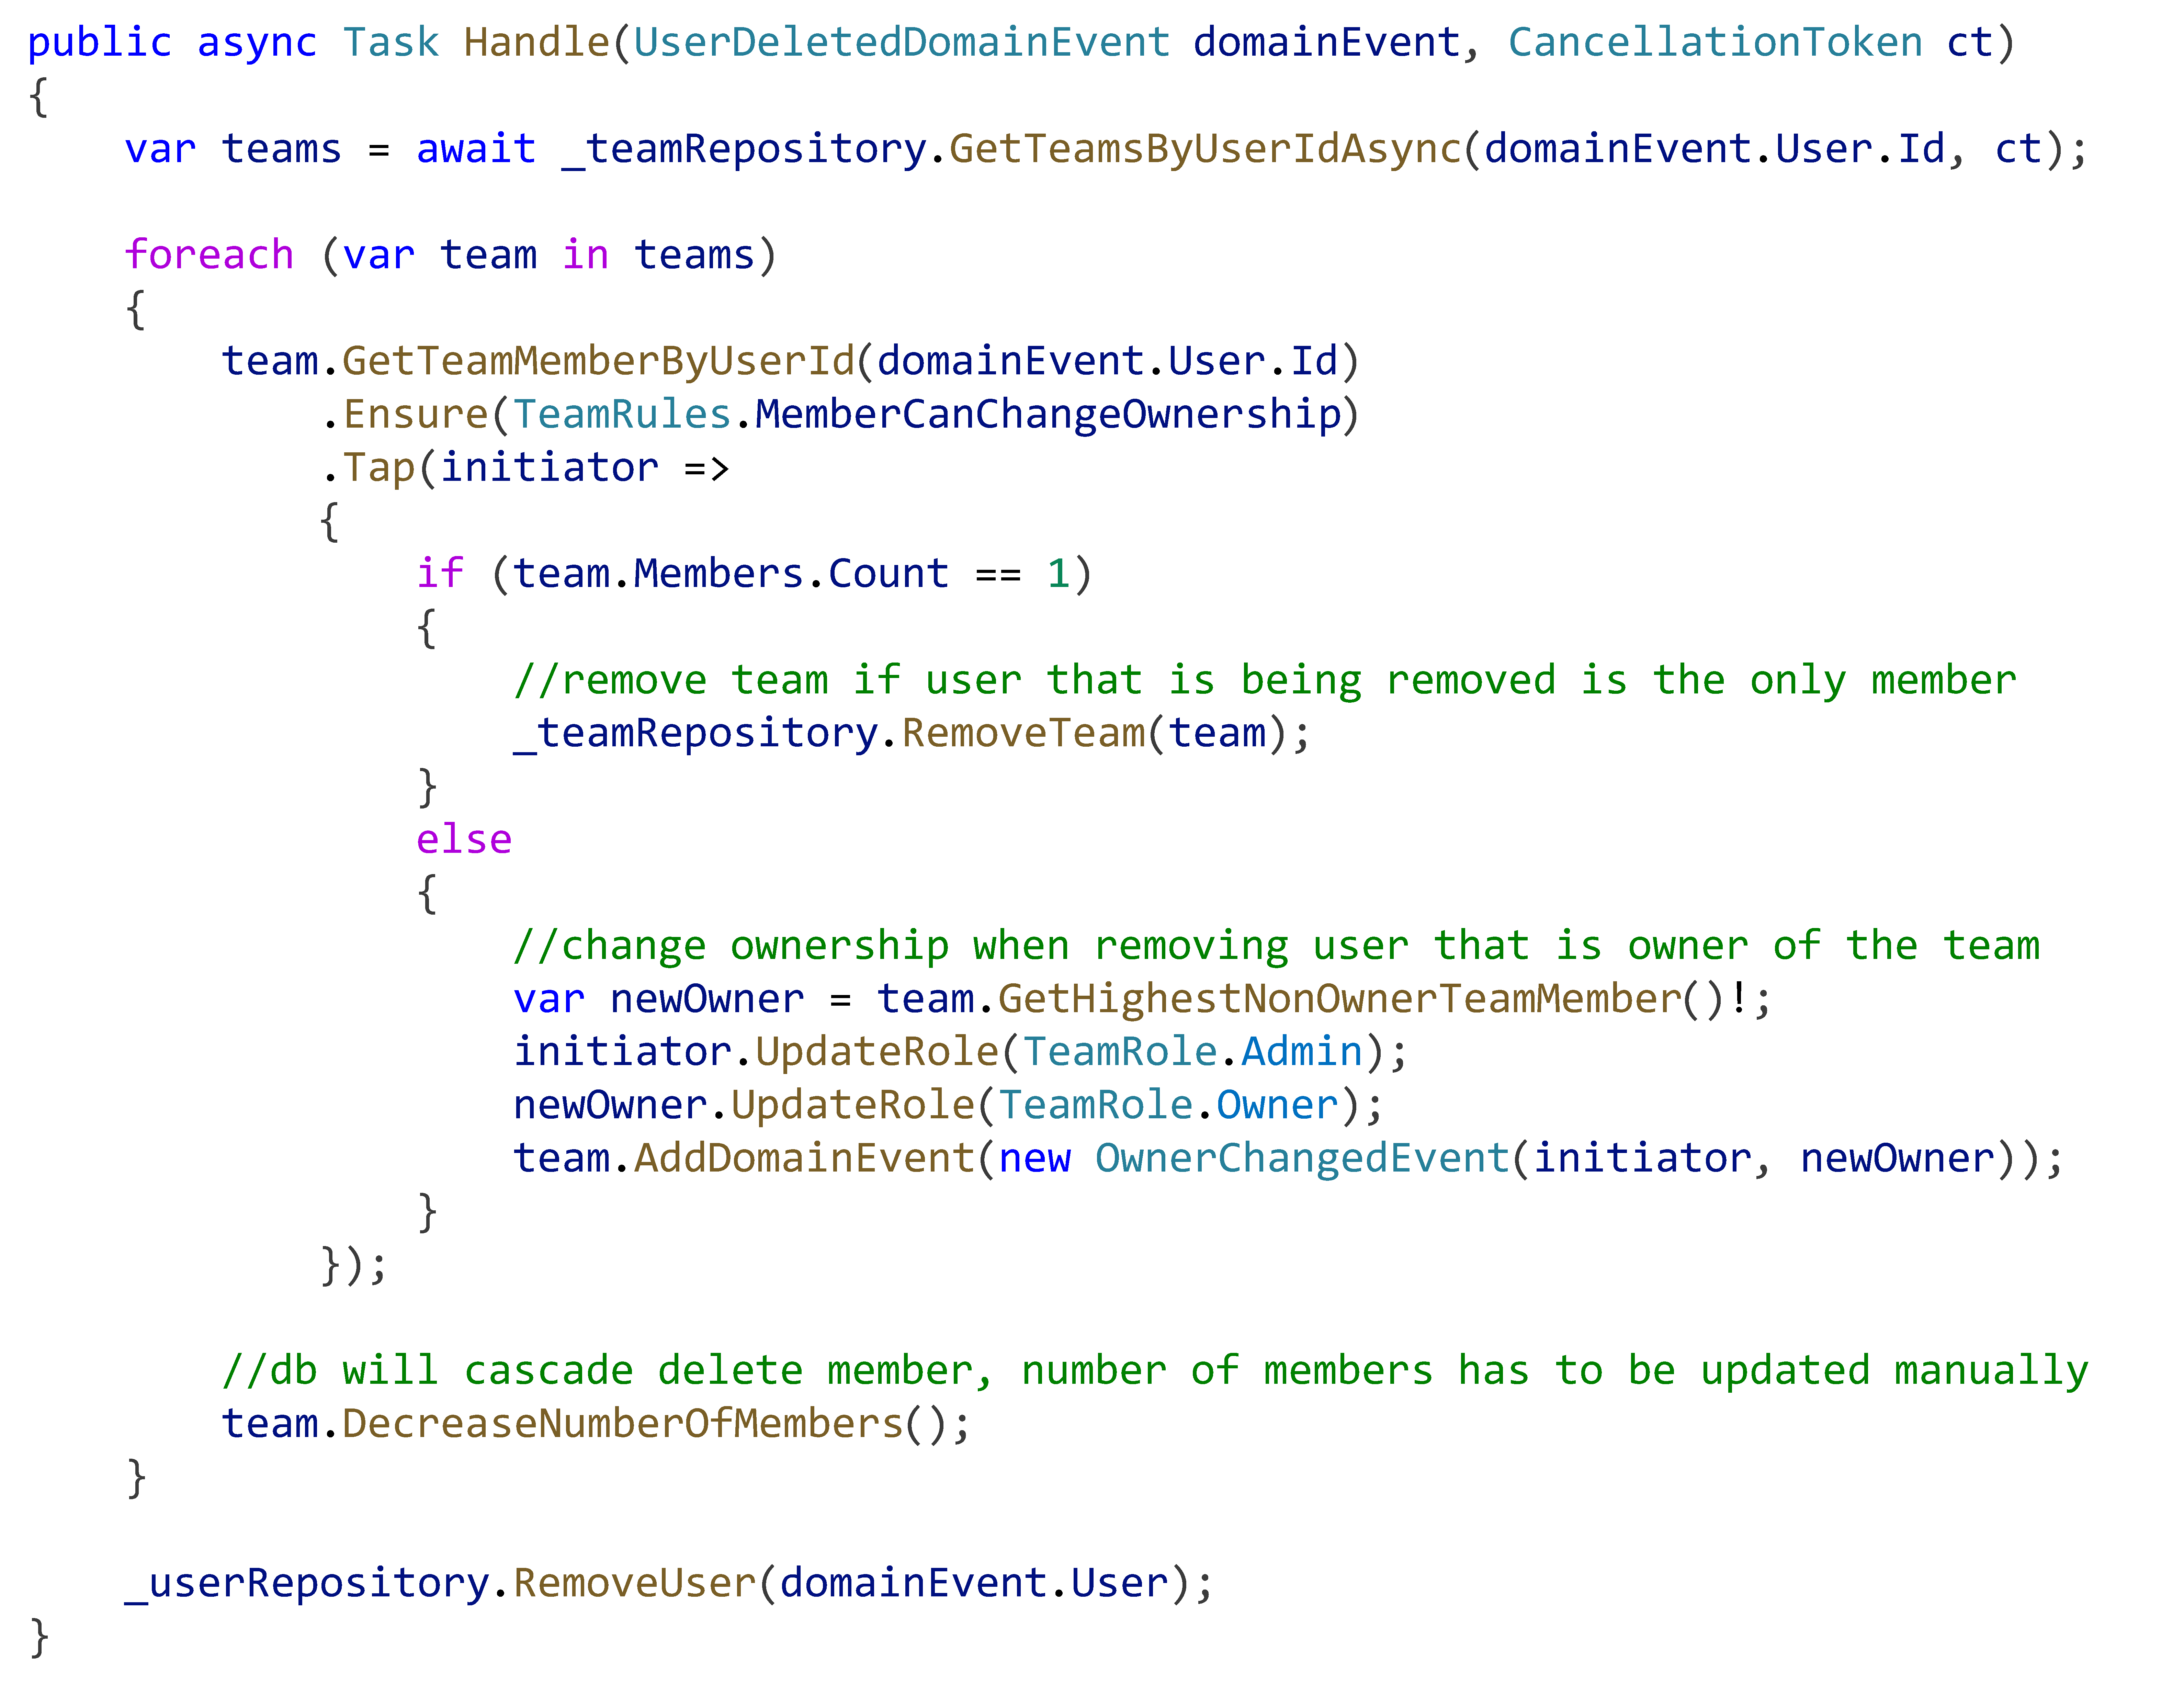
\includegraphics[width=\textwidth]{figures/doman-event-handler.pdf}
    \caption{Code sample of an event handler handling the \textit{user deleted domain event}.}
    \label{fig:domain_event_handler}
\end{figure}

\vspace{-7pt}
The event handler in figure \ref{fig:domain_event_handler} solves consistency problems resulting from the user deletion:
\begin{itemize}
    \item Deleting a team if the user is the only member (implicitly owner).
    \item Change ownership to another member if the user is the team owner (and raise an~\textit{ownership changed domain event}). This consistency problem could also be solved by~failing to delete the user if the user is an owner of a team, and the user would have to~manually change ownerships before deletion.
    \item Decreasing number of members in a team (required for race conditions, see \ref{dev:conccurency_conflicts}).
\end{itemize}

Deletion of team member records linked to the user is handled automatically by the RDBMS and db model with the \texttt{ON DELETE CASCADE} configuration.

\subsection{Application Layer}
The application layer contains implementation of application use cases, that is:

\begin{itemize}
    \item Implementation of commands and command handlers, which consists primarily of~calling the domain logic of aggregates, factories and domain services, and subsequently persisting the changes via the unit of work.
    \item Implementation of queries and query handlers, which consists of calling the query context façade around the EF Core context that builds and sends SQL queries, and subsequent validating of authorization rules (restricting what can be read by whom).
\end{itemize}

The sending requests (queries/commands) and processing them (handlers) is implemented using the \textbf{MediatR}\footnote{\url{https://github.com/jbogard/MediatR}} package, an in-process messaging mediator by Jimmy Bogard.

Additionally, the application layer contains helper services/interfaces and integration event handlers for performing asynchronous business actions (sending emails).

\begin{figure} [H]
    \centering
    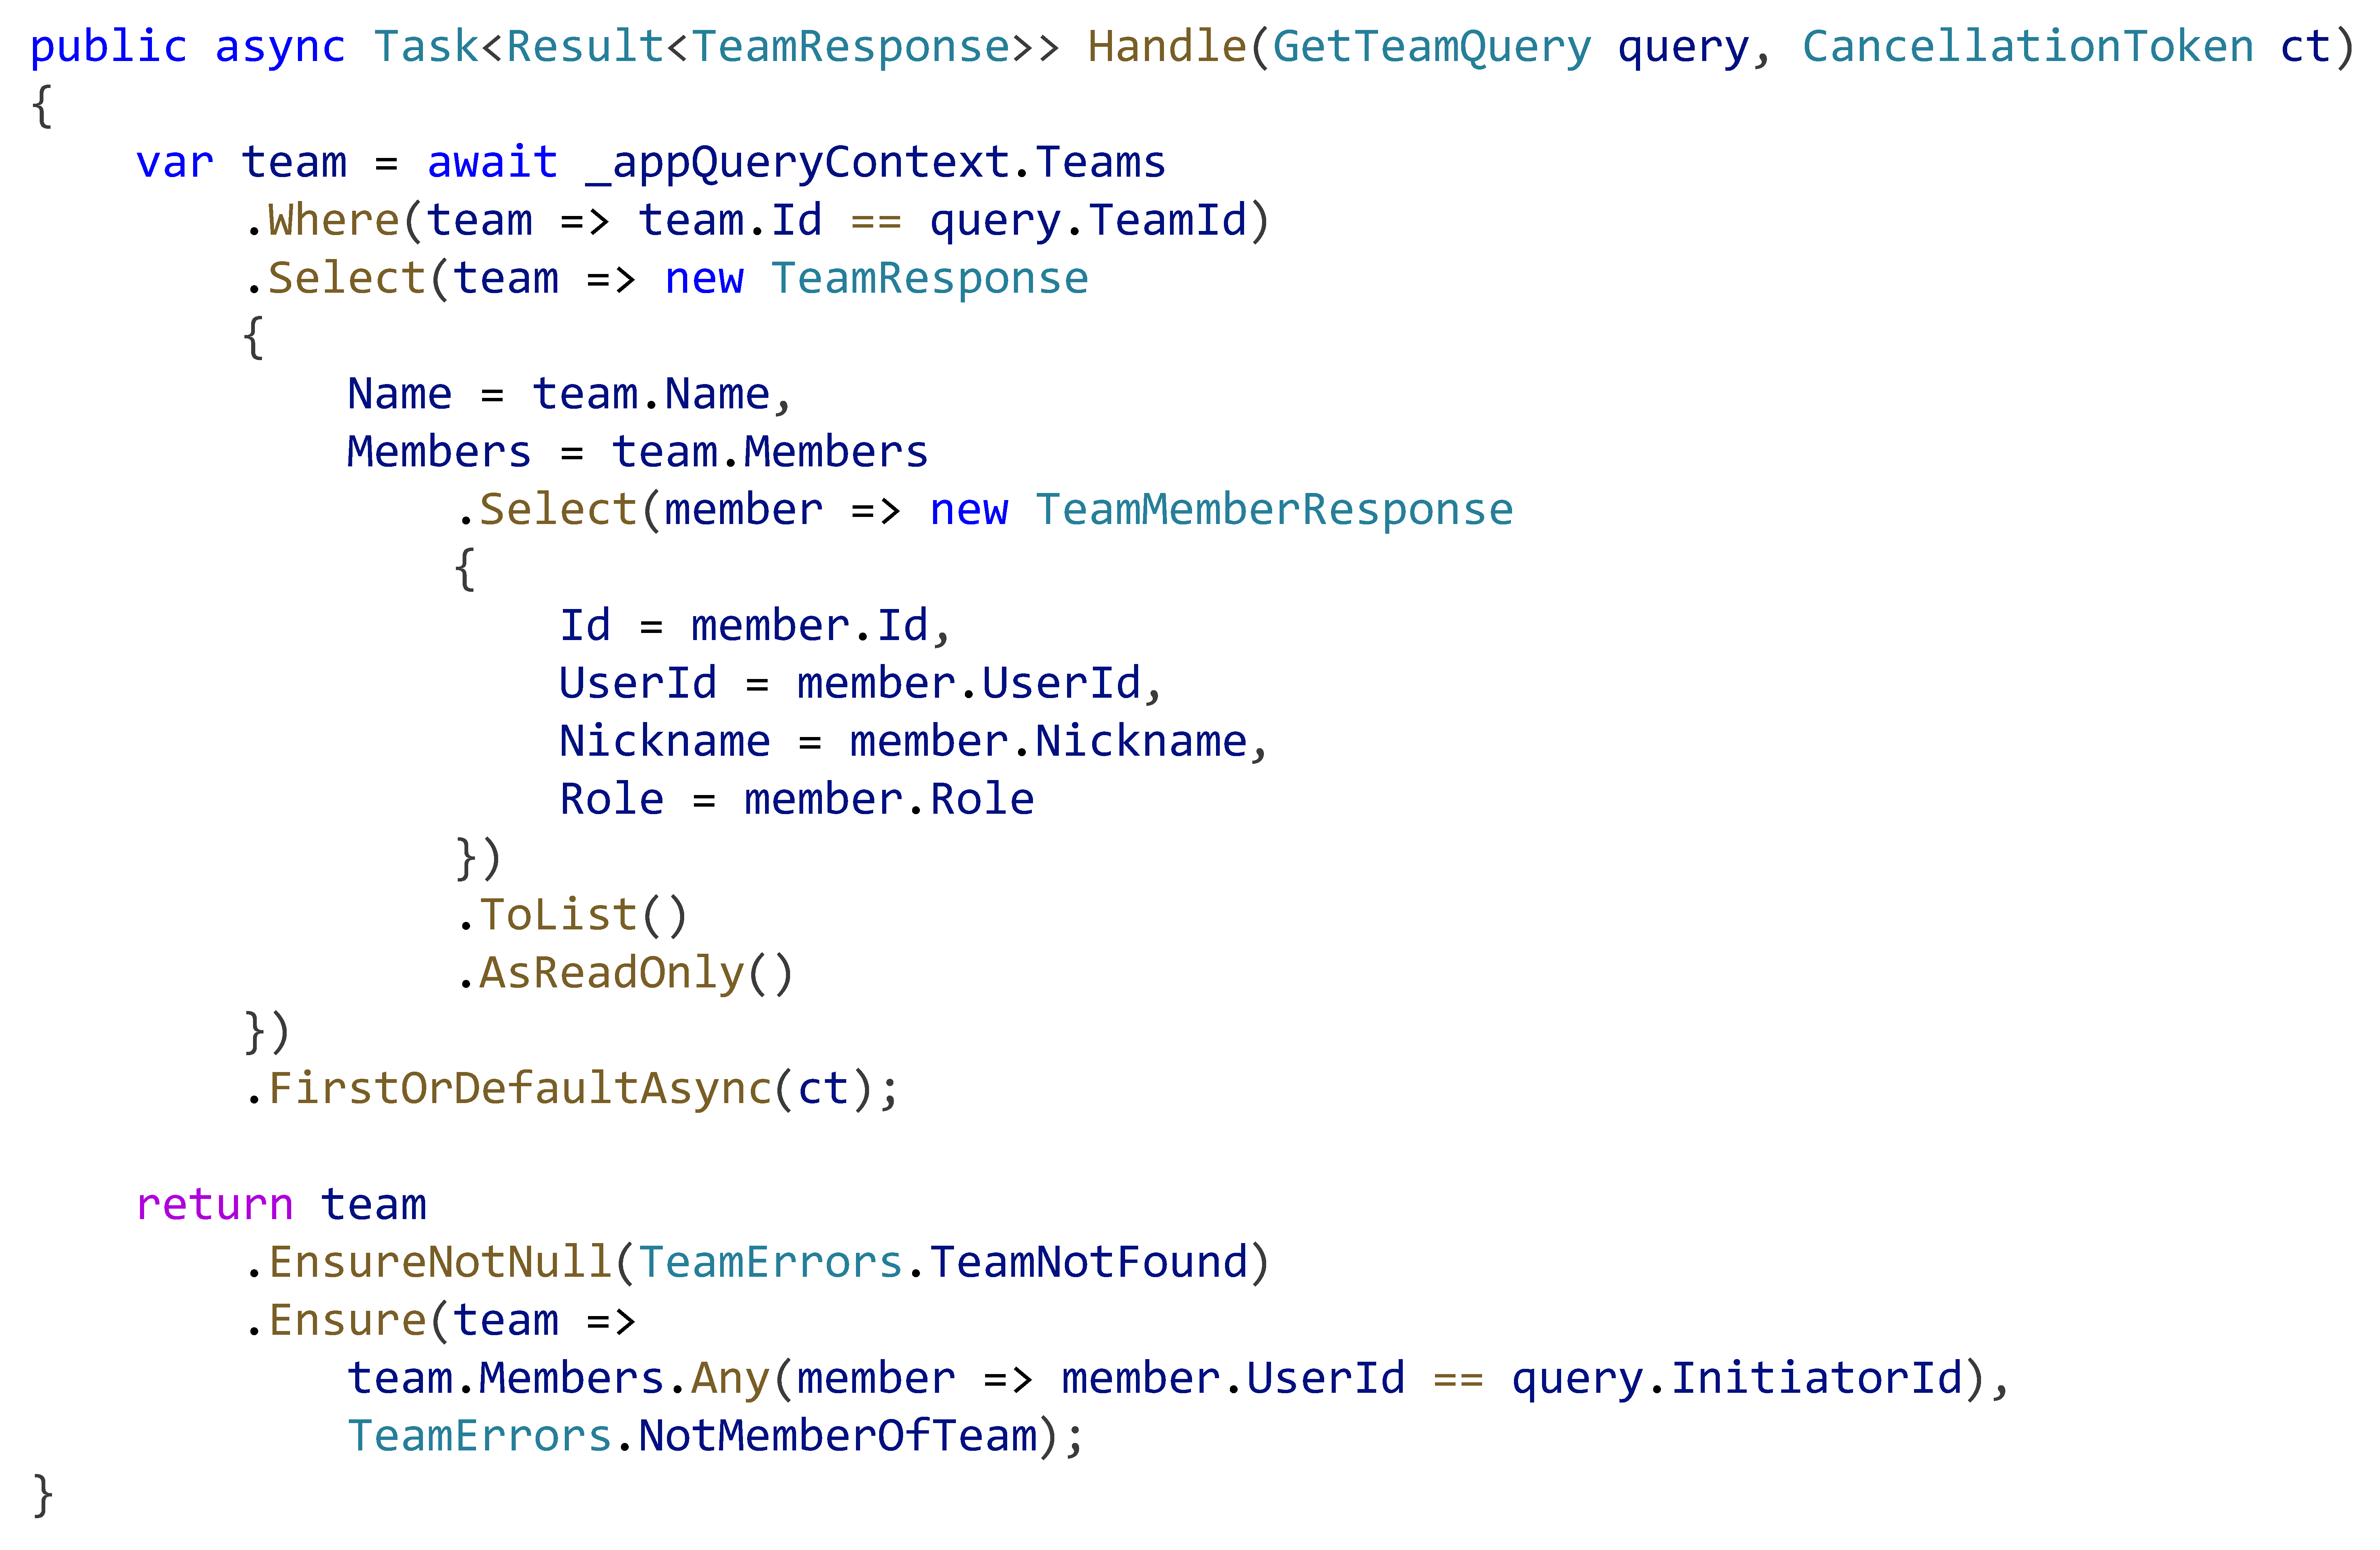
\includegraphics[width=\textwidth]{figures/query-handler.pdf}
    \caption{Code sample of a query handler of \texttt{GetTeamQuery} utilizing EF Core, where the EF Core builds SQL queries from given LINQ statements (and caches them for later reuse). After retrieving data from the database, the handler checks whether the team exists and whether the user is a member of the team. Note that the query statement uses \texttt{Select} to~map database result directly to desired response type (DTO).}
    \label{fig:query_handler}
\end{figure}

\subsection{Infrastructure Layer}
\label{dev:ca:infra}
The purpose of the infrastructure layer is to shield the application core from dependence on third-party libraries and external services, specifically by:

\begin{itemize}
    \item implementing core services (service abstractions from inner layers) including:
    \begin{itemize}
        \item \texttt{DateTimeProvider} -- it is considered a best practice to use a service to access date time as it provides an easy way to test logic involving date times.
        \item \texttt{UnitOfWork} -- since repositories and EF Core keep track of all changes to domain data, the unit of work exposes only the \textit{save changes} method to persist changes in a single transaction. Note that the method also ensures correct dispatching of all domain events raised within the transaction (see below).
        \item \texttt{QueryContext} -- essential for \textit{query handlers} because it enables to access database (no modification) by exposing \texttt{IQueryable} collections of the requested data (used to build LINQ queries that EF Core translates into SQL) with a \textit{no tracking} configuration, meaning EF Core will not track any changes to these objects.
        \\\dots
    \end{itemize}
    \item ensuring data persistence, that is, integrating database:
    \begin{itemize}
        \item Configuration of the domain objects (mapping the domain object definitions to~database tables) using the EF Core.
        \item Implementation of repositories -- integration to concrete database (postgres) using a specific technology (EF Core).
        \\\dots
    \end{itemize}
    \item integrating additional services, i.e. emailing service.
    \item implementing and configuring cross-cutting concerns, such as API security, dispatching integration events, and so on.
\end{itemize}

Structure: \vspace{6pt}
\dirtree{%
.1 TeamUp.Infrastructure/.
.2 Core/\DTcomment{implementation of core services}.
.2 Extensions/\DTcomment{extension classes used in the infrastructure layer}.
.2 Options/\DTcomment{option classes loaded from \texttt{appsettings.json}}.
.2 Persistence/.
.3 Domain/\DTcomment{entity configurations and repository implementations}.
.3 Migrations/\DTcomment{EF Core db schema migrations}.
.3 ApplicationDbContext.cs\DTcomment{EF Core database context}.
.3 DesignTimeDbContextFactory.cs\DTcomment{factory for creating migrations}.
.2 Processing/\DTcomment{processing services -- events, messages, etc.}.
.2 Security/\DTcomment{security concerns -- password service, JWT configuration, etc.}.
.2 AssemblyInfo.cs.
.2 ServiceCollectionExtensions.cs\DTcomment{methods for registering the layer into DI}.
.2 TeamUp.Infrastructure.csproj\DTcomment{assembly file}.
}

\subsubsection{Publishing Domain Events}
As previously mentioned, when a domain event is raised, it is collected from publishing at~the~end of~the~transaction. The collection is done by adding the event to the event list, and each entity has its own event list, hence, the domain events are bound to the entities that raised them, and the domain is not polluted with injection of service for raising/gathering domain events.

The \textit{unit of work} executes the actual publishing of the domain events as calling the \textit{save changes} method marks the end of the application transaction, another way may be by using EF Core interceptors to intercept \textit{save changes} and then proceed to publish events.

As mentioned in the segment about domain events (see section \ref{ddd:tactical_design} about DDD tactical design), they can be published within a transaction (single transaction for multiple aggregates) or asynchronously after committing one, making the system eventual consistent with multiple transactions when handling domain events.

I opted for \textbf{strong consistency} within a \textbf{single transaction}. In this application, eventual consistency would introduce unnecessary complexity and a single transaction involving multiple aggregates does not seem to cause any problems for this low scale application with few rather limited number of aggregates.

Problems with intensive locking when committing large transaction spanning multiple aggregates may be addressed by better domain modelling or by breaking the bounded context into modules and introducing eventual consistency between modules as in the Modular Monolith architecture, thereby reducing the transaction size.

\begin{figure} [H]
    \centering
    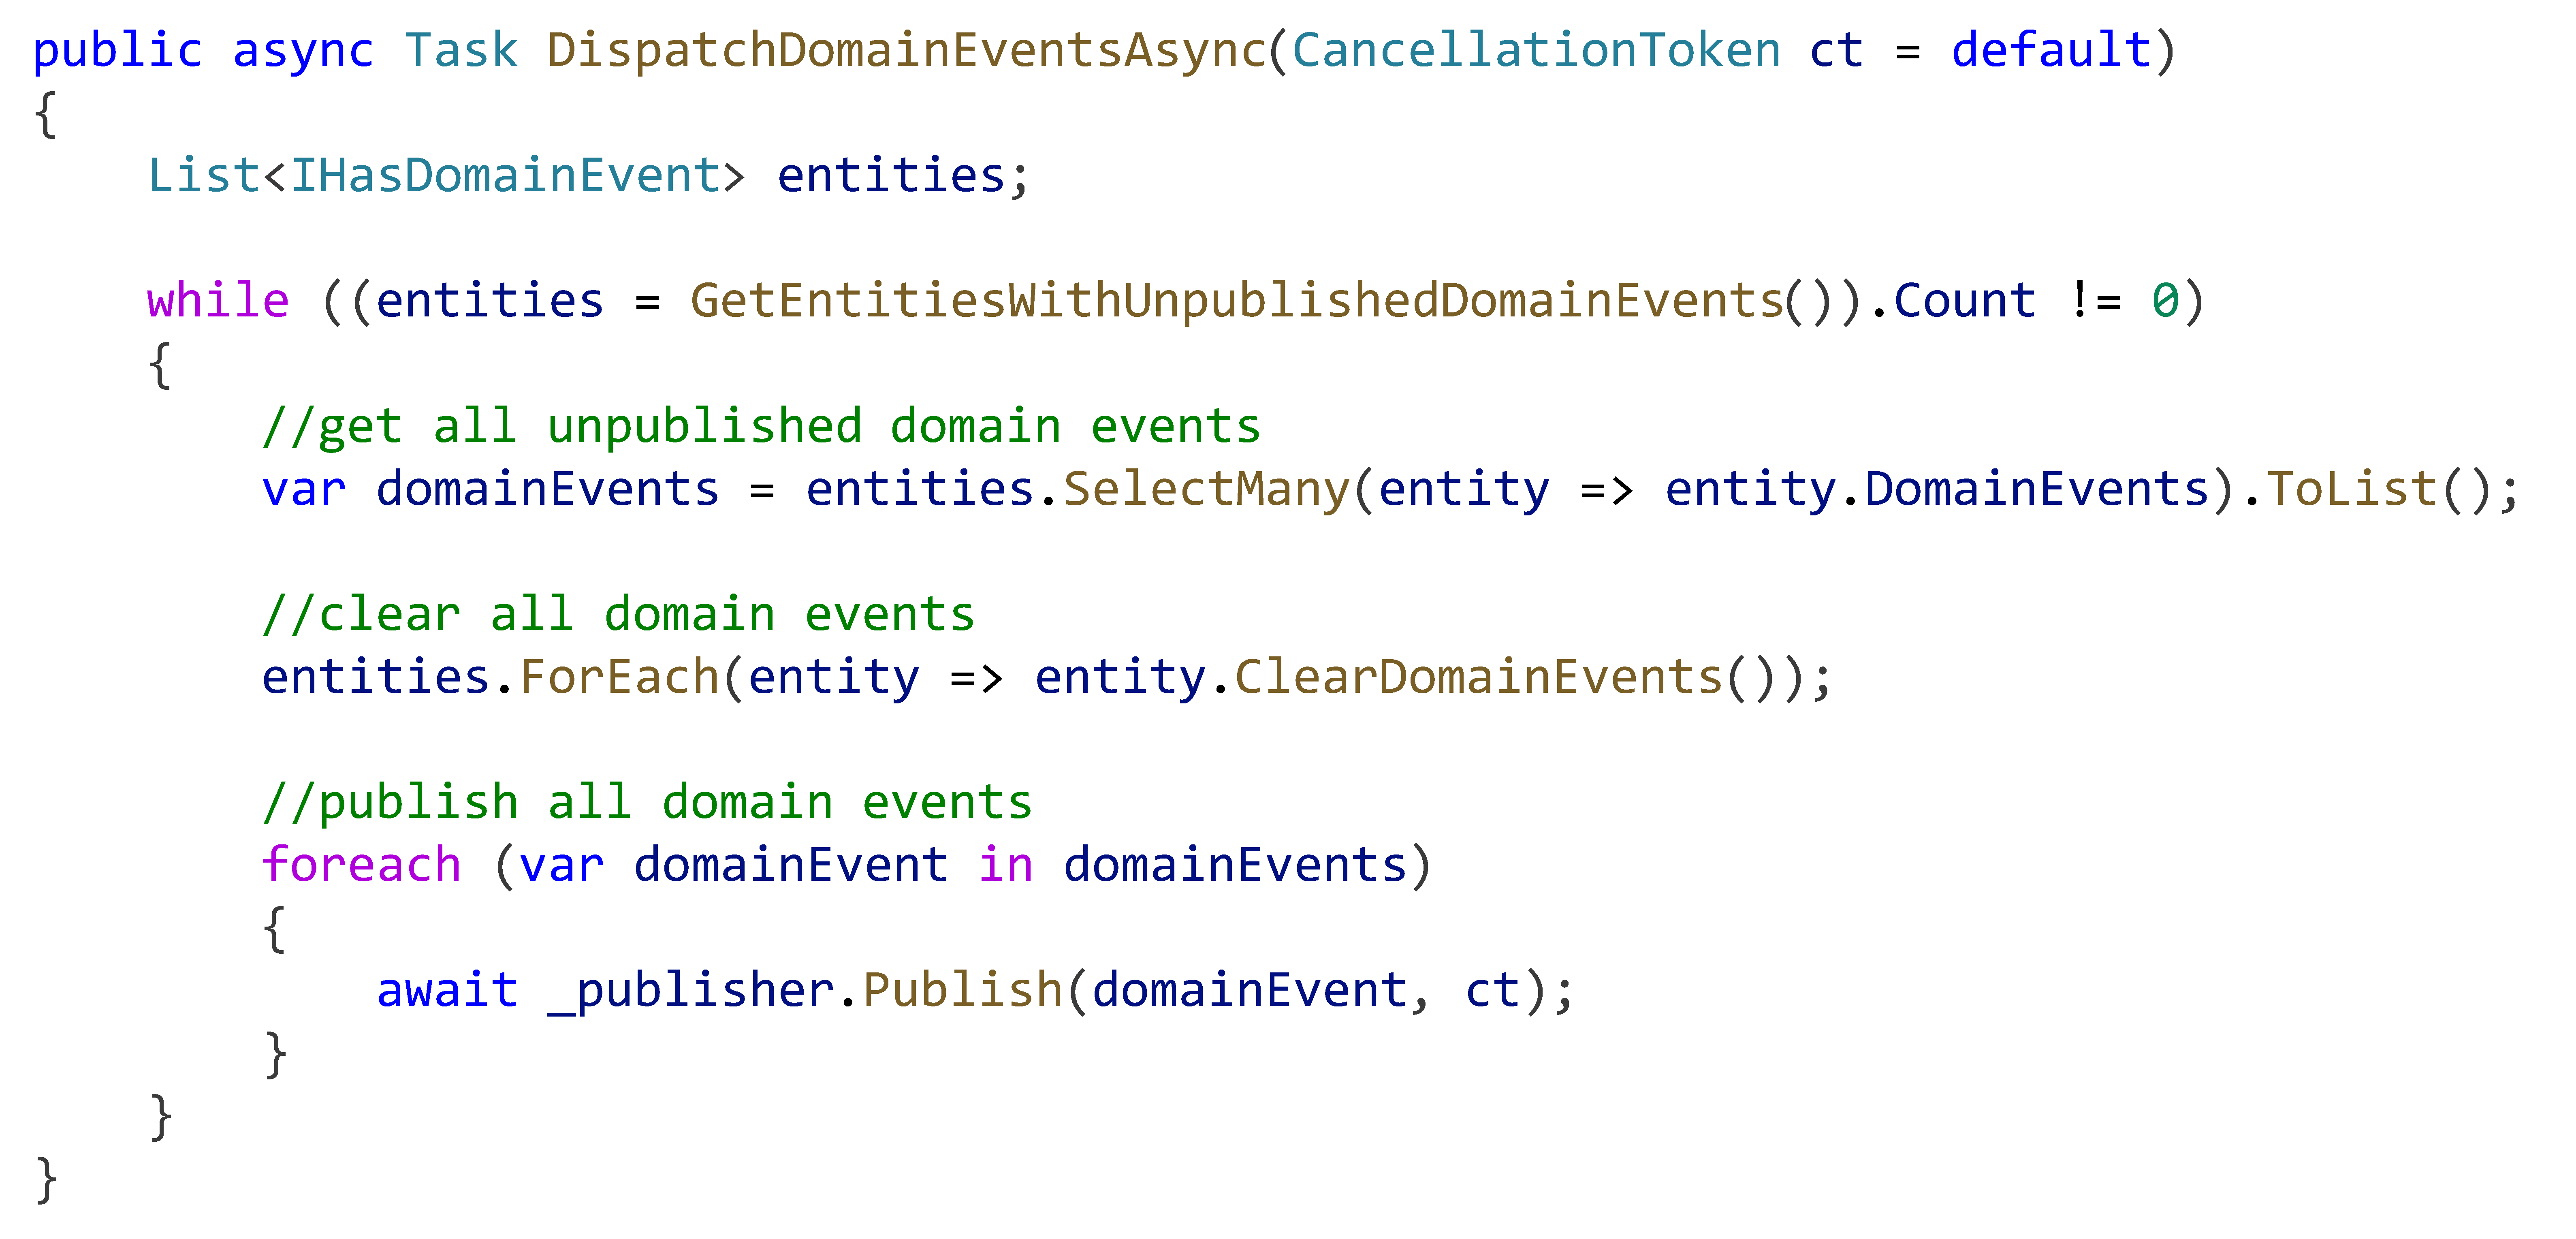
\includegraphics[width=\textwidth]{figures/dispatch-domain.pdf}
    \caption{Code sample for publishing domain events. The method for gathering entities with unpublished domain events uses the EF Core database context and \texttt{ChangeTracker} to~gather all changed objects that implement \texttt{IHasDomainEvent} interface and whose event list is not empty. Note that the loop repeats until all domain events are published as~event handling may produce additional events that were not initially gathered. This could lead to a potential infinite loop, but hopefully it would be detected by the integration tests.}
    \label{fig:dispatch_domain_events}
\end{figure}

\subsubsection{Outbox \& Publishing Integration Events}
To reliably handle asynchronous side effects -- integration events -- a transactional outbox pattern has to be used (see section \ref{theory:outbox} about outbox pattern).

This means that the side effect producer has to raise an integration event from a domain event handler (or possibly from a domain service) using the \texttt{IntegrationEventManager}, the idea being that since side effects affecting the database are processed inside domain event handlers, asynchronous side effects should be raised from them as well.

Since integration events are serialized into outbox messages, they do not contain object references, but only direct values or references via identifiers (uuid/guid).

\begin{figure} [H]
    \centering
    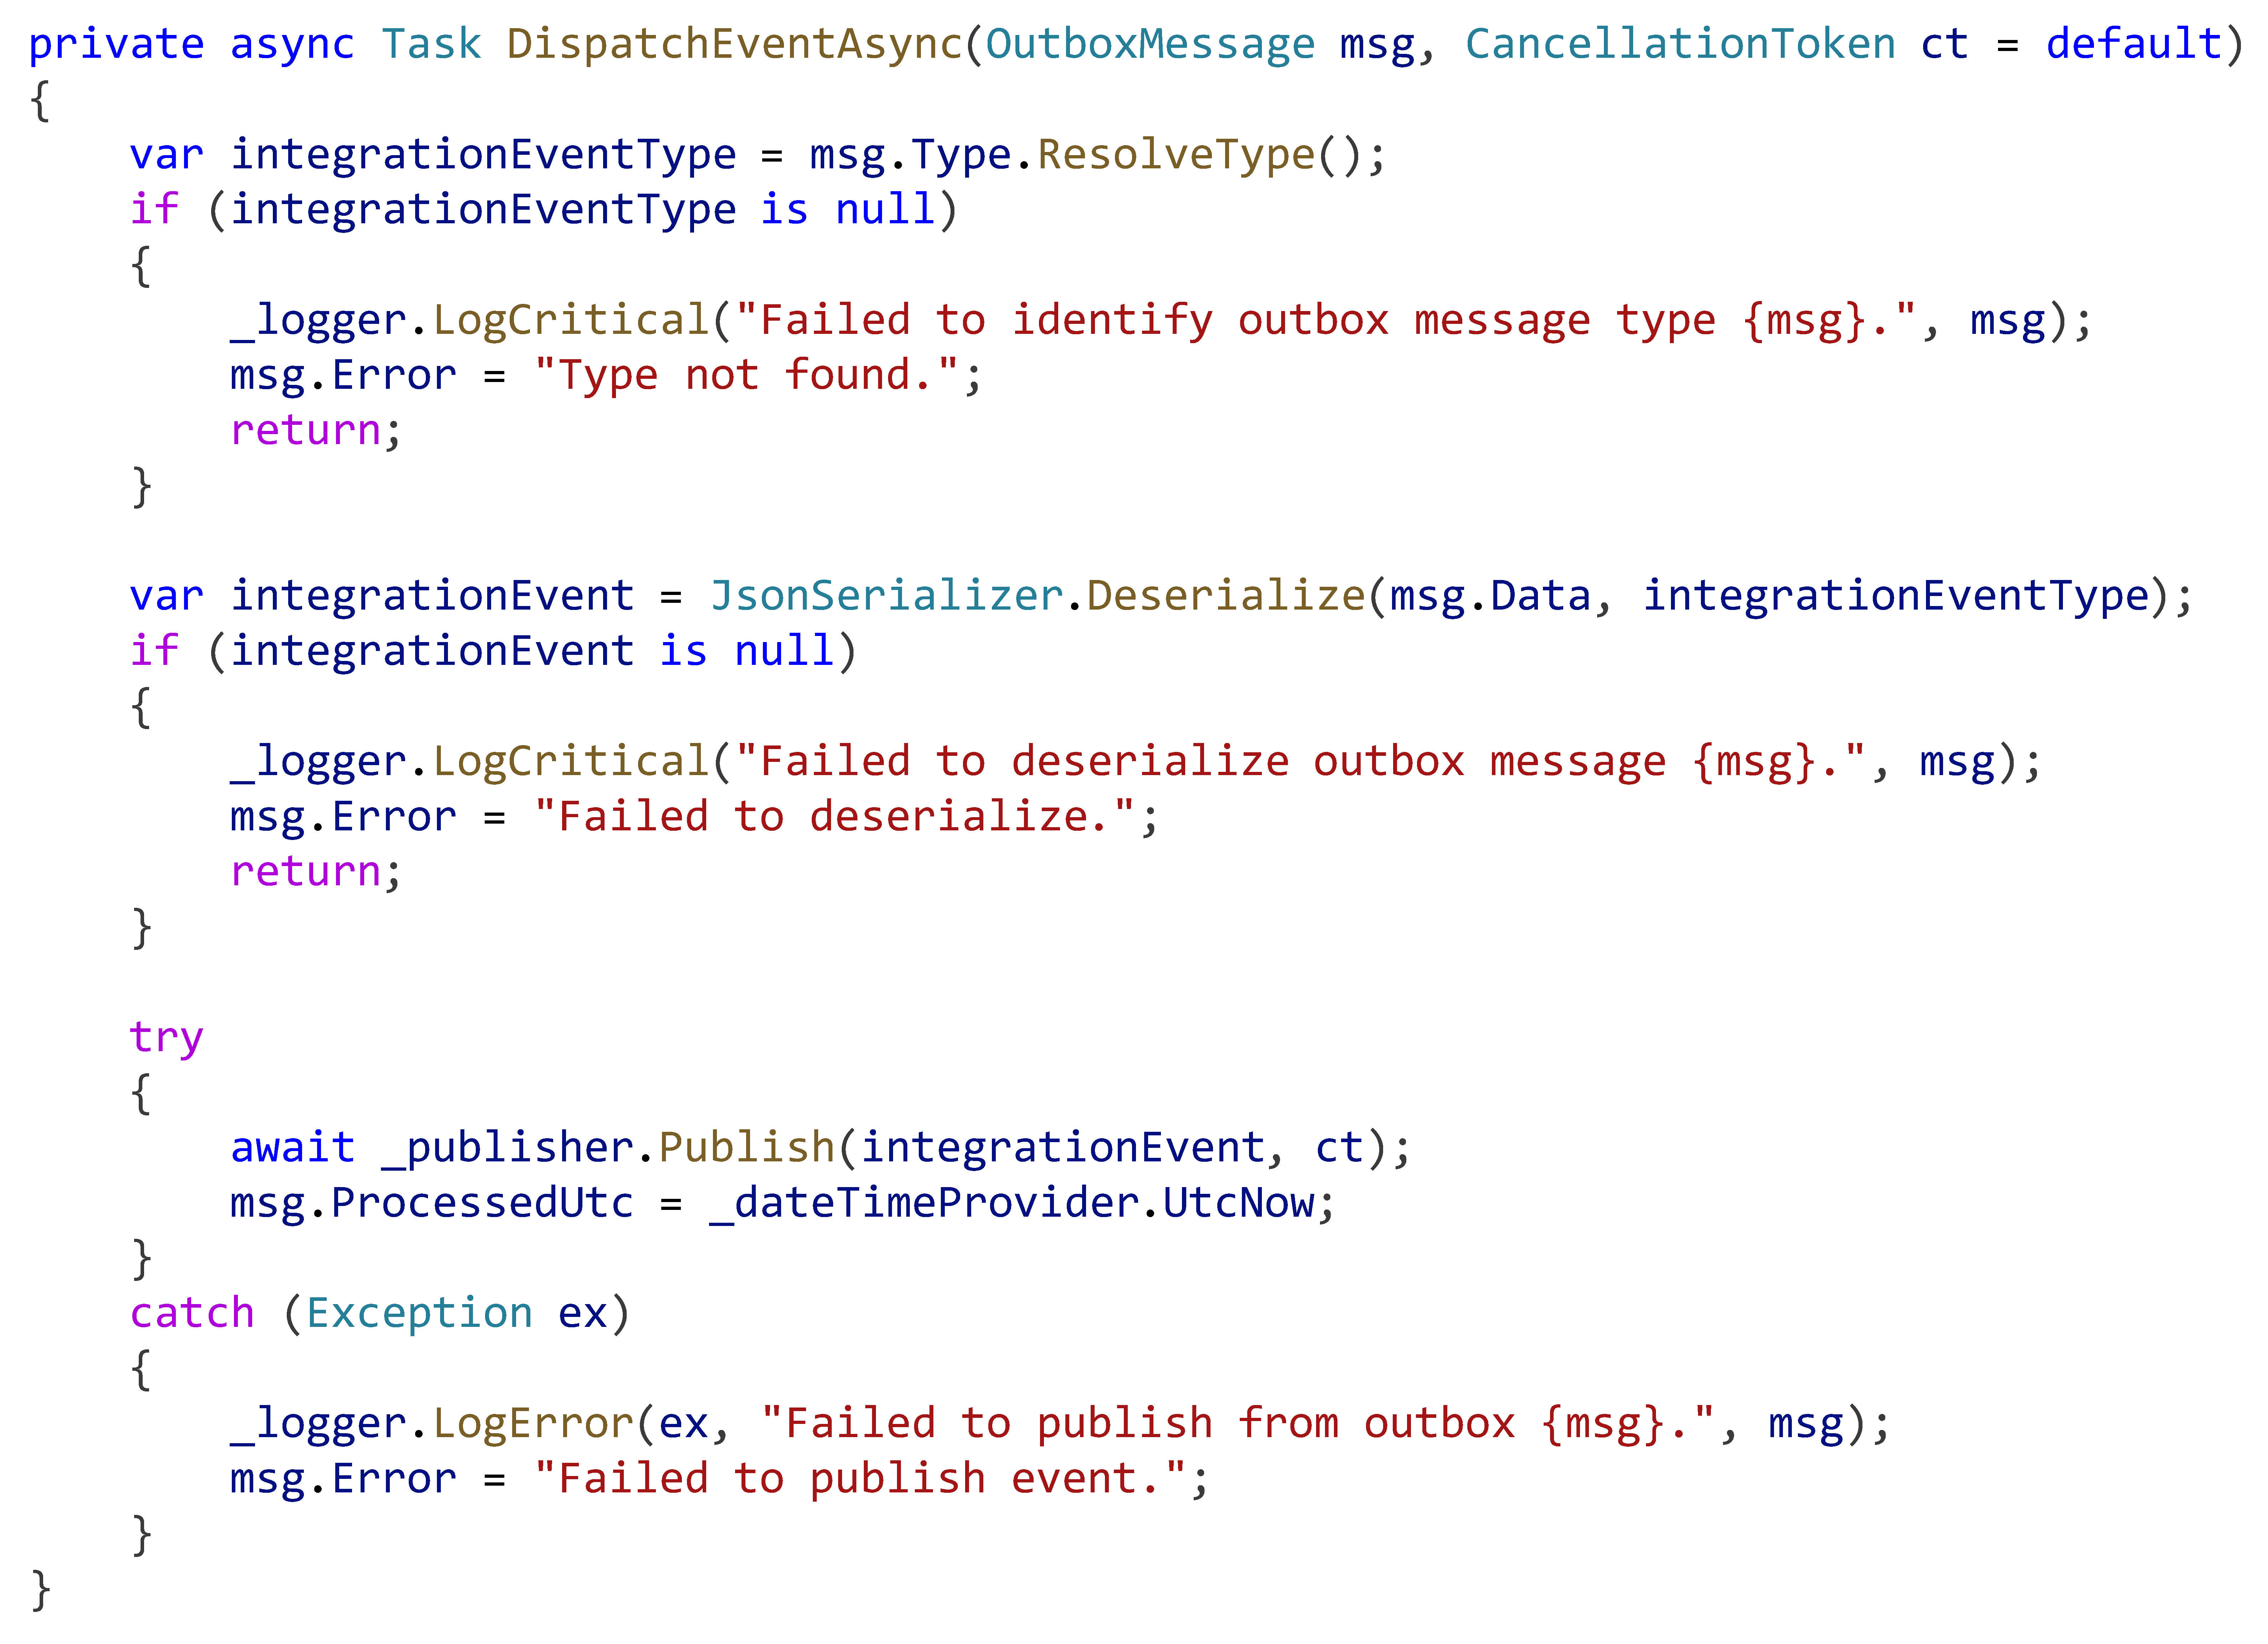
\includegraphics[width=\textwidth]{figures/dispatch-integration.pdf}
    \caption{Code sample for dispatching a integration event from an outbox message. By~updating the \texttt{ProcessedUtc} property, the outbox message is marked as~published. If an error occurs during the consumption of outbox message or while publishing an event, the step in which the error occurred is logged and stored in the db.}
    \label{fig:dispatch_integration_events}
\end{figure}

Publishing integration event workflow goes as follows 
\begin{enumerate}
    \item Integration event producer serializes event and persists it into the outbox within transaction caused by a command.
    \item Every M seconds, the outbox processor takes N unconsumed messages, deserializes them and publishes them; successfully consumed messages are marked as processed in the outbox, failed ones will be re-consumed in the next iteration.
\end{enumerate}

\newpage
\subsection{Presentation Layer}
The presentation layer contains application entry point with building and configuring the~server using the ASP.NET Core framework:
\begin{itemize}
    \item Configuration of server components (authentication, API versioning, etc.) and registration of services into DI container via extension methods from individual layers.
    \item Application of required middlewares, for example for routing, authentication, authorization, CORS, and so forth.
    \item Mappings of RESTful endpoints that call application logic via commands and queries. Endpoints are decorated for automatic generation of OpenAPI\footnote{\url{https://swagger.io/resources/open-api/}} specification.
    \item Addition of development-specific parts (development-only) such as swagger (for demo testing API), logging middlewares, automatic database migrating, etc.
\end{itemize}

\begin{figure} [H]
    \centering
    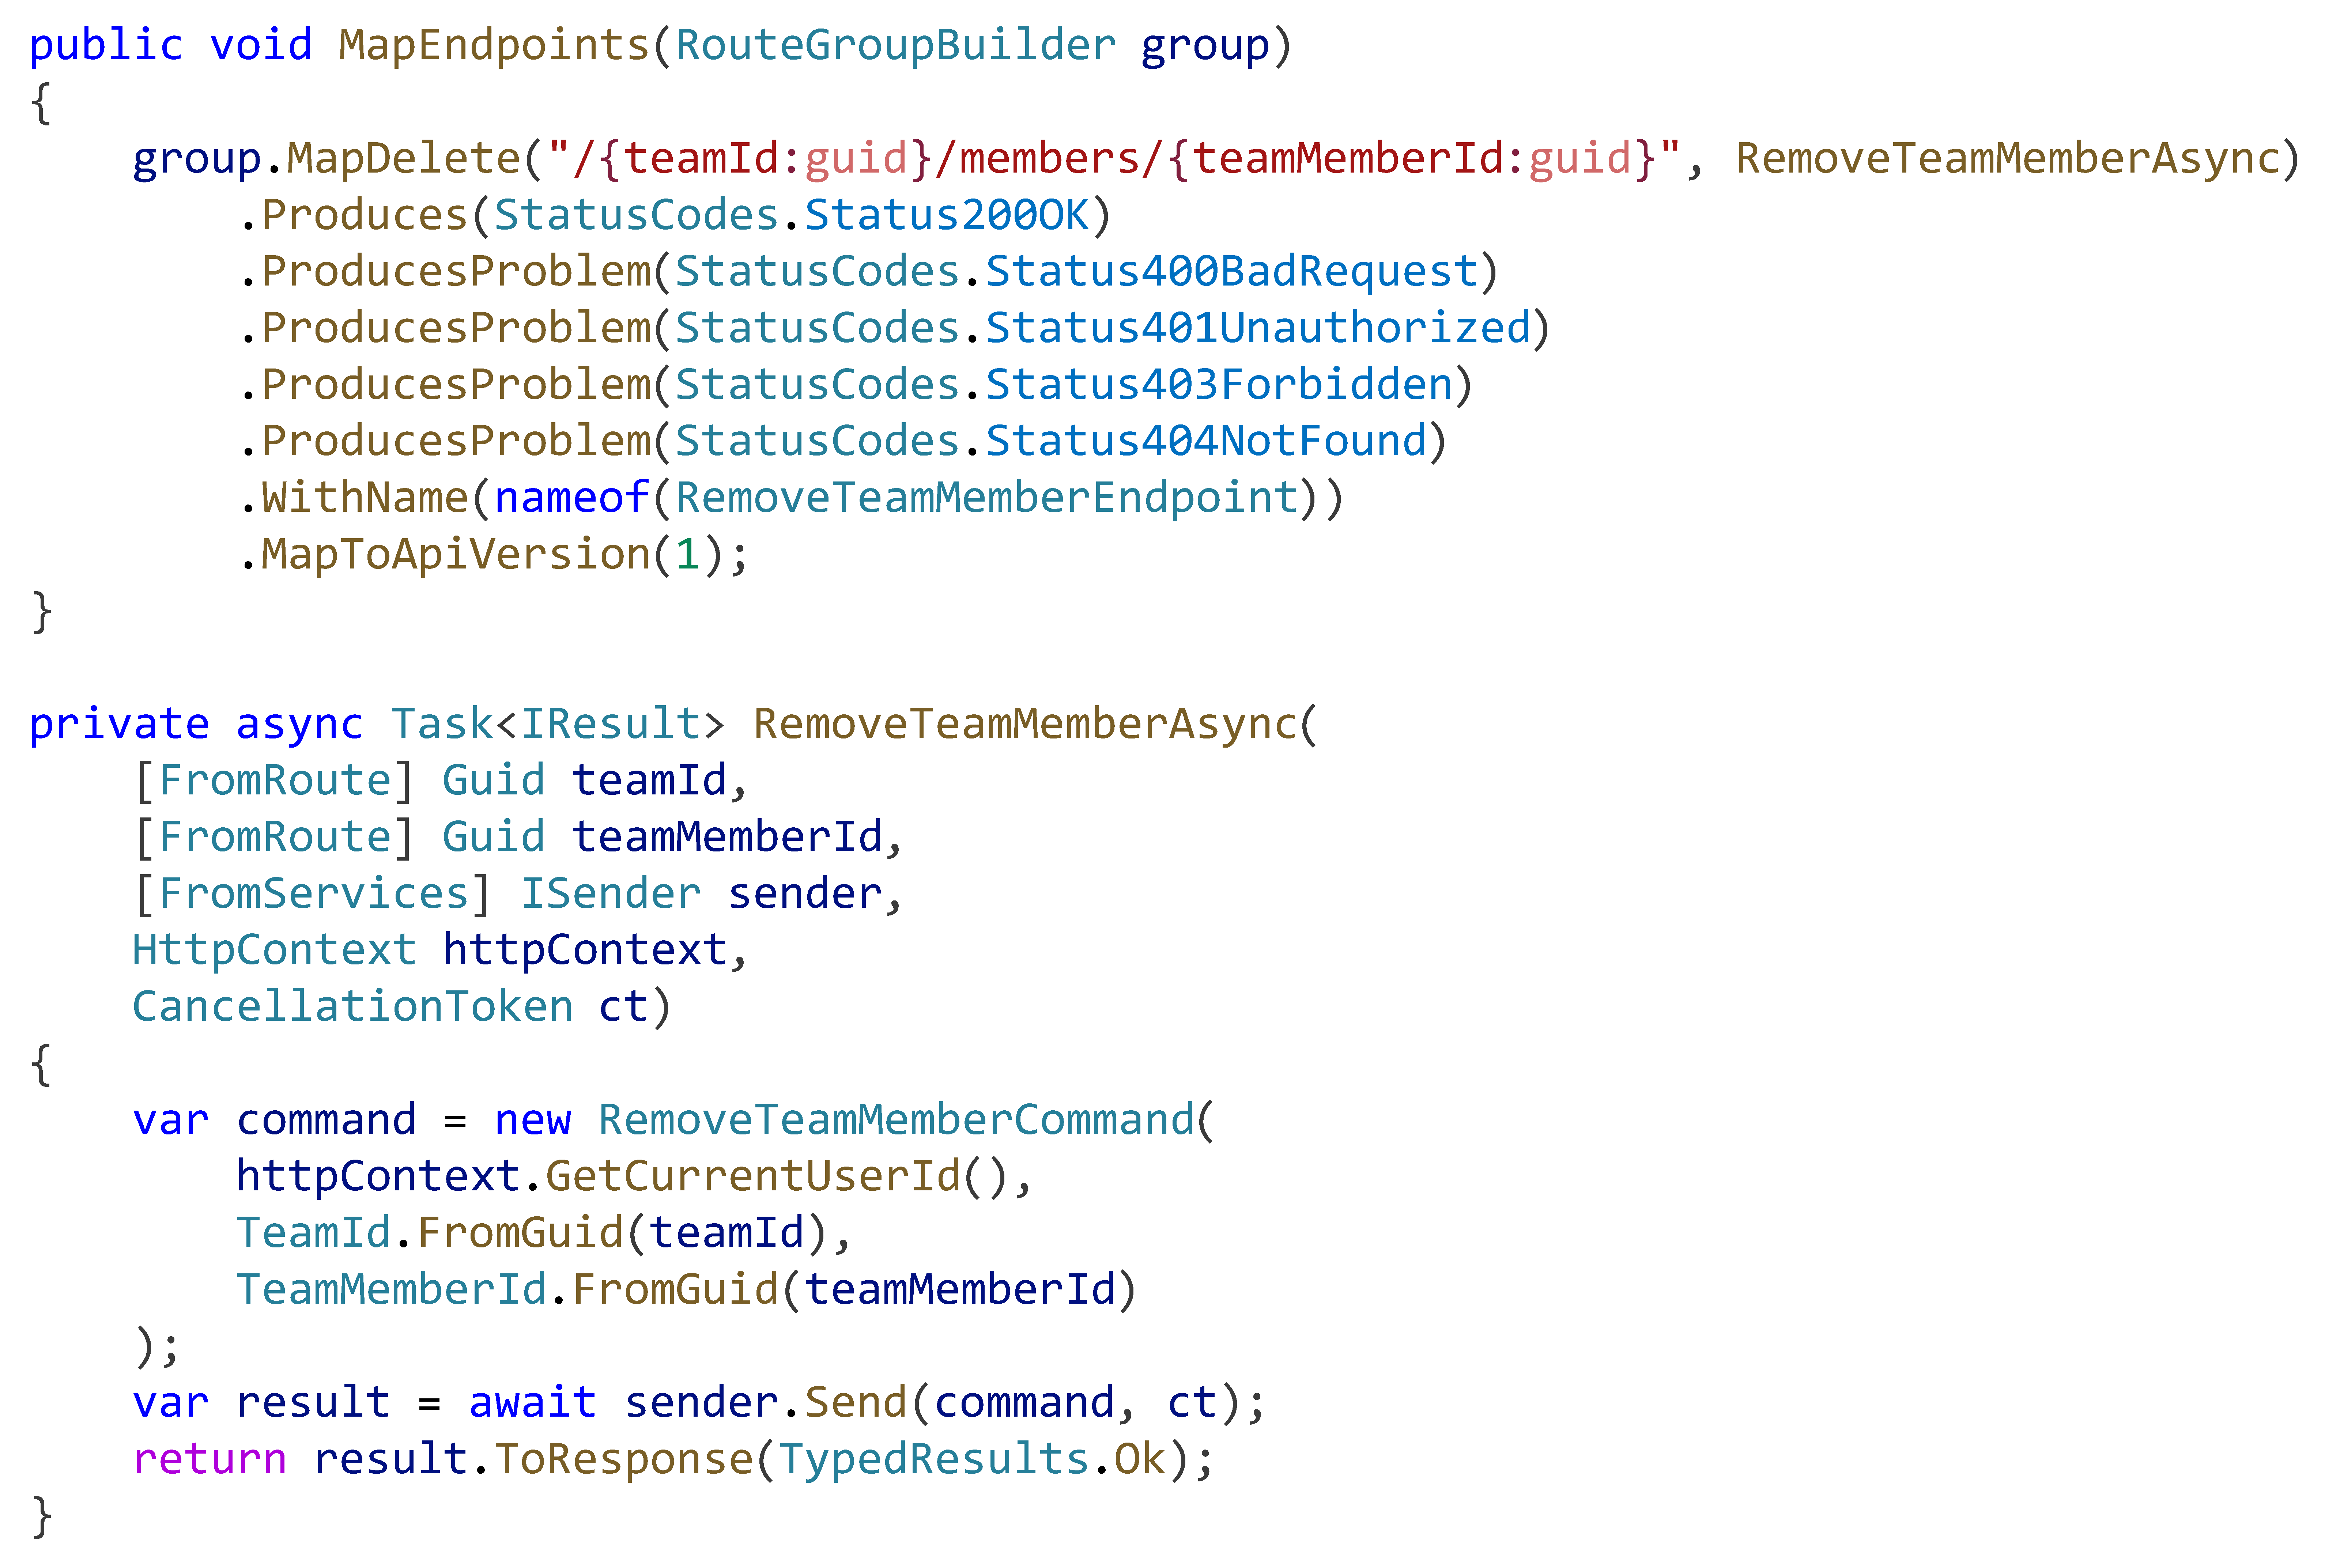
\includegraphics[width=\textwidth]{figures/endpoint.pdf}
    \caption{Code example of an endpoint for removing a team member from the team. The~\texttt{MapEndpoints} method utilizes the dotnet functionality (\textbf{Minimal API}{\protect\footnotemark}) to map endpoints, and additional methods for automatic generating of the OpenAPI specification. The~\texttt{RemoveTeamMemberAsync} method is an actual endpoint handler that creates a command/query from the http context (request parameters, headers, etc.), calls the application logic via the command/query, and maps the result to the correct http response.}
    \label{fig:endpoint}
\end{figure}
\footnotetext{\url{https://learn.microsoft.com/en-us/aspnet/core/fundamentals/minimal-apis}}

\subsection{Invite unregistered user workflow example}

\begin{figure} [H]
    \centering
    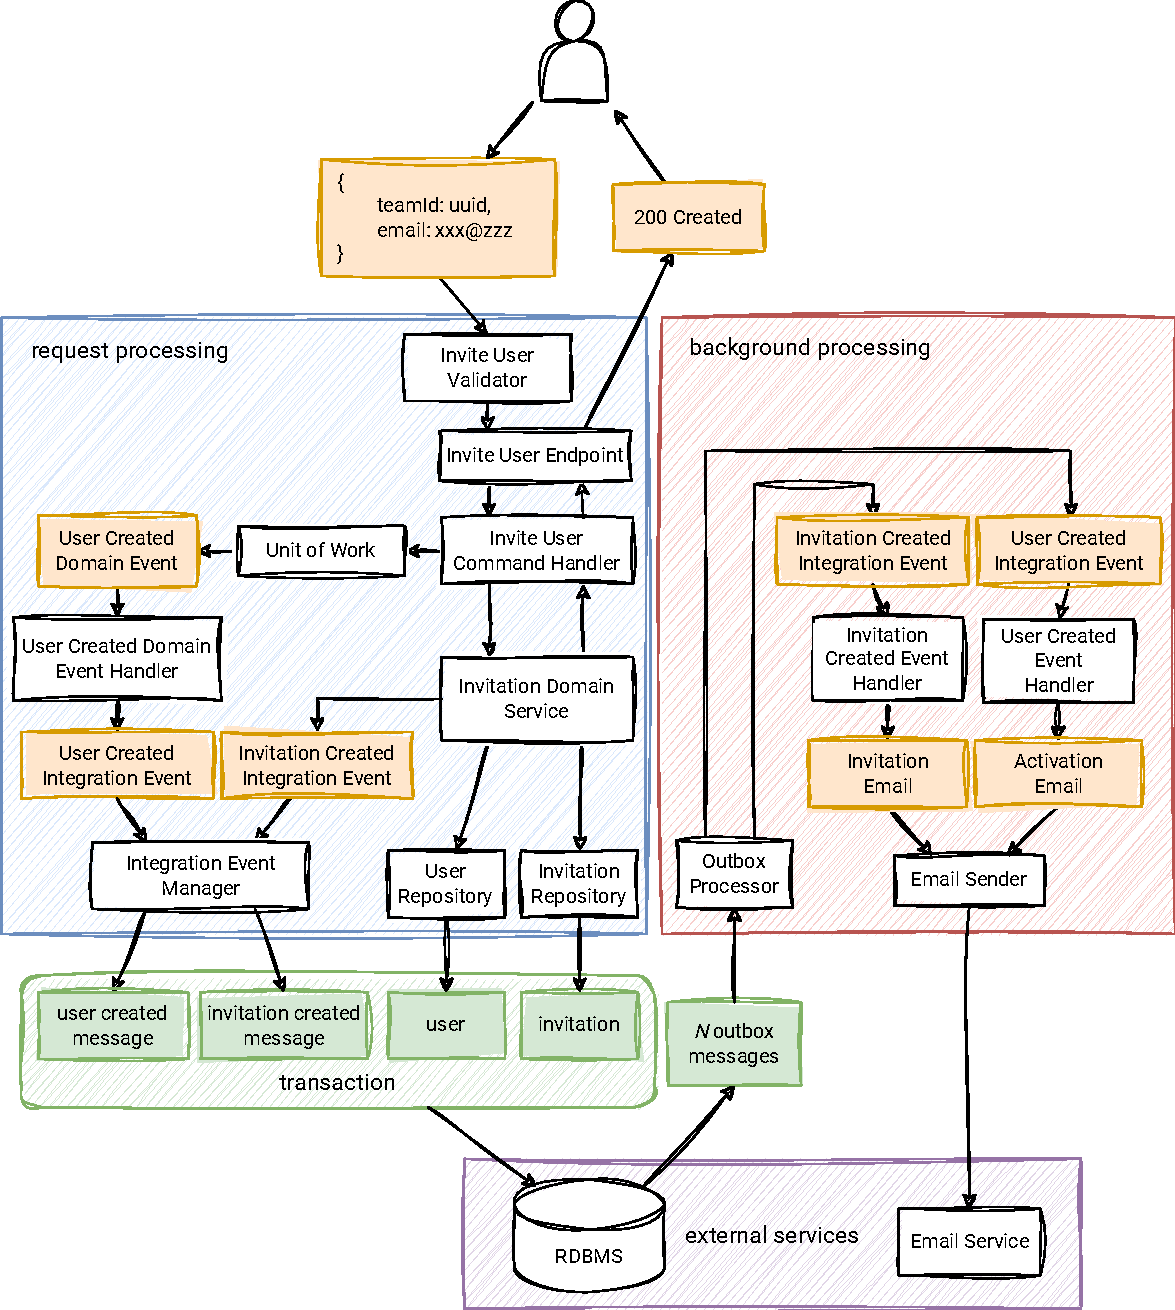
\includegraphics[width=\textwidth]{figures/ca-workflow.pdf}
    \caption{Diagram showing the workflow of inviting a user that is not registered to~a~team, assuming all data is valid. Diagram outlines key components that the workflow goes through and the events that are published along the way. Note that the transaction is committed by the \textit{unit of work} and before committing, the \textit{user created domain event} is collected and published. This diagram skips the API authorization process.}
    \label{fig:ca_workflow}
\end{figure}

\newpage
\section{Modular Monolith solution}
\label{dev:modular_monolith}
The entire Modular Monolith solution is available online as a repository on GitHub:

\url{https://github.com/skrasekmichael/ModularMonolith}

\subsection{Identifying modules}
Appropriate decomposition of the system into modules is crucial for system maintainability and scalability, each module should be independent of others and focus on its own functionality.

To some extent, module decomposition mirrors the DDD strategy design (bounded context = module), although even a bounded context can be divided into multiple modules if it is advantageous (smaller modules = smaller transactions).

The core modules can be supplemented by supporting modules that cover highly distinct or specific functionality from other modules, such as infrastructure integration (SMS gateway, etc.), data processing (pdf, image, video, etc.), and so on.

\subsubsection{Modules}
\begin{itemize}
    \item \textbf{User Access Module} -- mirrors the functionality for the business needs of the User Access bounded context.
    
    \item \textbf{Team Management Module} -- mirrors functionality and business needs of~the~Team Management bounded context. It might be beneficial to split this module into more sub-modules (for instance, a separate module for invitations), however, it should be easy to decompose it in later development iterations.

    \item \textbf{Notifications Module} -- encapsulates the functionality for notifying users (currently only by email) via special services/technology.
    
    The existence of a separate module allows for easy addition of notification methods (e.g. sms) and in case of transition to microservices, each microservice does not need to have its own notification infrastructure, but can use this internal service for pushing notifications instead.

    \item Bootstrapper -- entry point to the application bootstrapping all modules, necessary services and configurations to a single executable (ASP.NET Core app). When migrating to microservices, this module would be turned into an API gateway/reverse proxy.
\end{itemize}

\subsection{System Design}
The system is designed for easy transition to microservices in the context of data modeling, isolation and communication patterns incorporating eventual consistency.

Each module that provides data manipulation functionality integrates the CQRS pattern, with the queries being lightweight database calls and commands leveraging DDD for complex business logic (similarly to the Clean Architecture solution design in section \ref{dev:ca:deisgn}).

\subsubsection{Communication}
Communication between modules is primarily \textbf{asynchronous}, facilitated over a \textbf{message broker} (see figure \ref{fig:mm_design}). This approach ensures loose coupling between modules. Each module exposes contracts, such as integration events, for external communication. Internally, modules communicate synchronously using in-process calls.

To support more complex interactions, the system also registers request-response paths over the message-broker, enabling synchronous (blocking) command and query invocations between modules. This allows to call commands or queries of other modules when necessary. Furthermore, the input validation is moved to the command/query handlers to validate incoming communications not only from external sources but also from other modules, ensuring robustness and consistency across the system.

To ensure reliable communication and consistency, each module has its own storage for~outbox and inbox (see section \ref{theory:outbox} describing transactional outbox pattern), even if a~module does not have to persist state to execute its logic. Implementing this demand resulted in~some problems (see more in segment about multiple outboxes in section \ref{problem:multiple}).

\subsubsection{Data Isolation}
Data isolation is achieved via a \textbf{separate schema} per module in a \textbf{single database} (see figure \ref{fig:mm_design}). Since the system does not contain cross-schema transactions, there is no data coupling between modules, providing sufficient isolation akin to microservices. 

\begin{figure} [H]
    \centering
    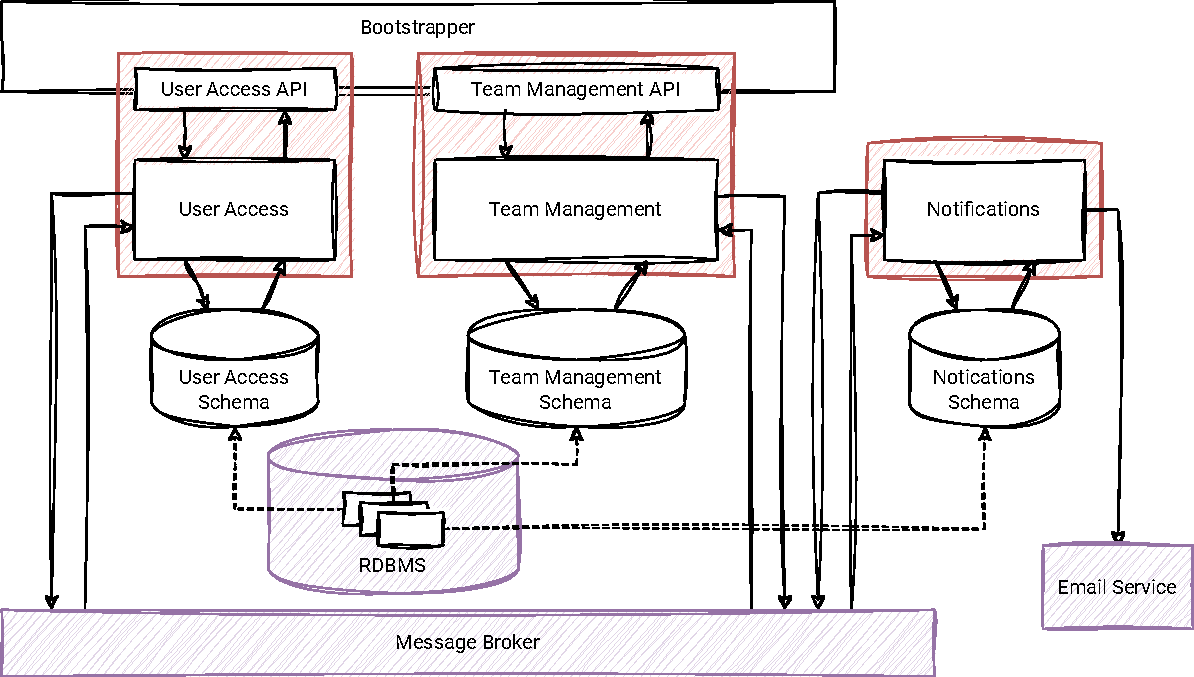
\includegraphics[width=\textwidth]{figures/mm-design.pdf}
    \caption{Diagram showing data isolation, communication between modules (red) and integration with infrastructure services (purple). Note that each module also has background processing services, which are omitted from this diagram for simplicity.}
    \label{fig:mm_design}
\end{figure}

\subsection{Implementing solution}

\begin{itemize}
    \item Message Broker: \textbf{RabbitMQ} as a reliable messaging and streaming broker without cloud vendor lock-in. Popular non-cloud specific alternatives are Apache Kafka, ActiveMQ or Redis. 
    \item Communication framework: \textbf{MassTransit} is popular open-source distributed application framework for .NET, providing a consistent abstraction on top of the supported message transports (RabbitMQ, Amazon SQS, Azure Service Bus, etc.). Popular alternatives to MassTransit are NServiceBus or Wolverine.
\end{itemize}

Project structure: \vspace{6pt}

\dirtree{%
.1 TeamUp/\DTcomment{Modular Monolith repository}.
.2 src/.
.3 Common/\DTcomment{shared types and building blocks}.
.3 Modules/.
.4 UserAccess/\DTcomment{user access module layers}.
.4 TeamManagement/\DTcomment{team management module layers}.
.4 Notifications/\DTcomment{notifications module layers}.
.3 TeamUp.Bootstrapper/\DTcomment{entry point assembly}.
.2 tests/.
.2 TeamUp.sln.
.2 \dots.
}

\subsubsection{Modules Separation}

Each module is organized with a clean architecture-like structure, composed of required layers and optional layers tailored to its functionality:
\begin{itemize}
    \item \textbf{Contracts Layer} containing all types and abstractions necessary for communication with a given module (commands and queries, response types, integration events, etc.).
    
    \item \textbf{Application Layer} with the logic of the module
    
    \item \textbf{Infrastructure Layer} containing the module's abstraction and services for configuring, registering, and using the module.
    
    \item Optional \textbf{Endpoint Layer} if module exposes REST API endpoints.

    \item Optional \textbf{Domain Layer} for modules that work with domain objects applying the~rich domain model and DDD principles.
\end{itemize}

Each layer type within a module utilizes building blocks and common types, shared across assemblies for~a~consistent and reusable layer implementation = a common assembly for each layer type (see figure \ref{fig:mm_assemblies}).

The \textbf{Bootstrapper} assembly then links all the modules and assemblies together (see figure \ref{fig:mm_bootstrapper}), establishing the application's architecture, initiating runtime environment, and providing application entry point as ASP.NET Core app.

The higher number of assemblies creates a vast amount of interconnecting dependencies, which can lead to linking incorrect dependencies. To avoid dependency hell, each layer must follow strict rules on which assemblies it can depend on (shown in figure \ref{fig:mm_assemblies}); for~enforcing these rules, see section \ref{dev:arch_testing} on architecture testing.

\begin{figure} [H]
    \centering
    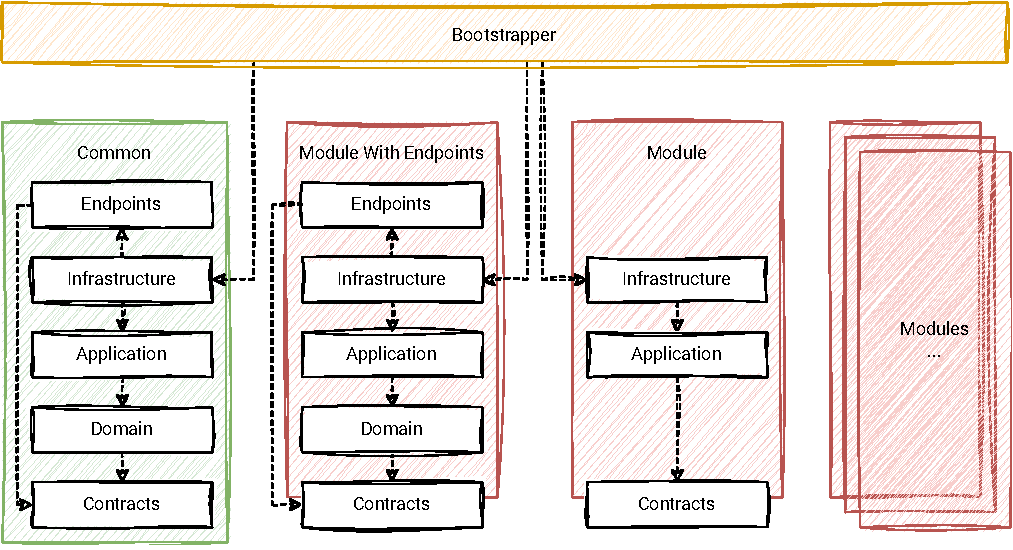
\includegraphics[width=\textwidth]{figures/mm-assemblies.pdf}
        \caption{Diagram indicating the separation of modules and assemblies and the dependencies between them. Each module can depend on contracts of any module. Note that each layer in a module always depends on the corresponding common layer assembly; these dependencies are excluded from the diagram to make it more readable (dependencies are implied by the same row position).}
    \label{fig:mm_assemblies}
\end{figure}

\begin{figure} [H]
    \centering
    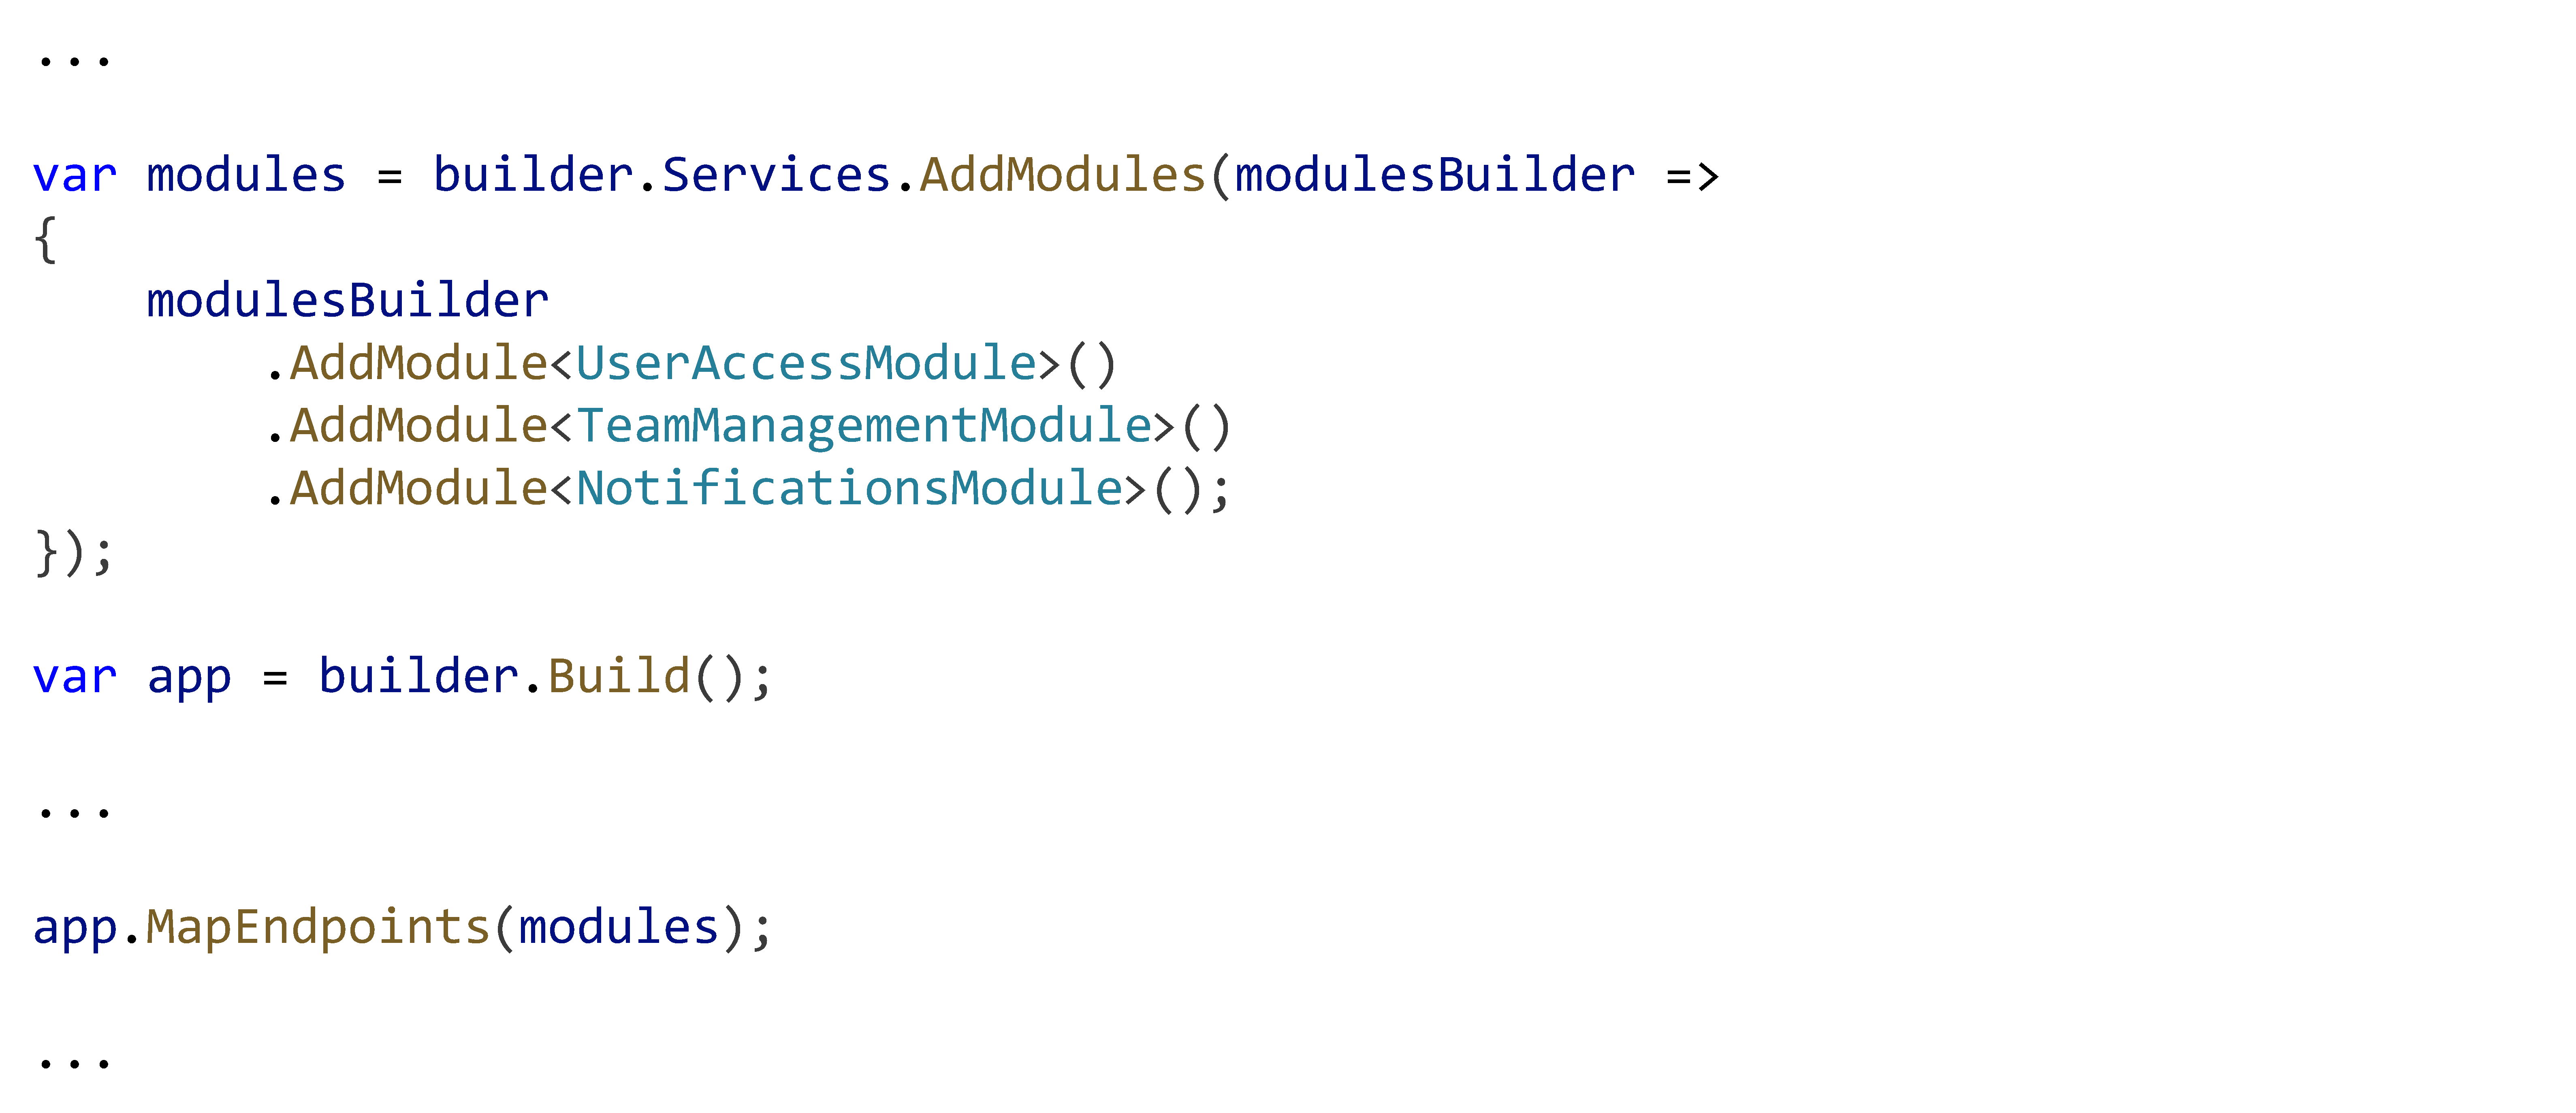
\includegraphics[width=\textwidth]{figures/bootstrapper.pdf}
    \caption{Code from the bootstrapper assembly demonstrating the registration of modules (configurations, service implementations, etc.) and endpoint mapping using an automated process built around module abstractions (see below).}
    \label{fig:mm_bootstrapper}
\end{figure}

\subsubsection{Module Abstraction}
Each module (logical boundary) defines a module (class) in its infrastructure layer, where a module can inherit one of 2 base class implementations:
\begin{itemize}
    \item \texttt{ModuleWithEndpoints<ModuleId, ModuleDbContext, ModuleEndpointGroup>} \\for~a~general module exposing REST API endpoints.
    \item \texttt{Module<ModuleId, ModuleDbContext>} for internal module.
\end{itemize}

The module then only needs to implement \texttt{ConfigureServices} method for registration of~module specific services (and some layer information about assemblies) and based on~those, the~base class automatically registers/configures all required services, that is:
\begin{itemize}
    \item command/query and event handlers
    \item MassTransit consumers for commands, queries and integration events
    \item essential services such as db context, unit of work, background jobs \dots
\end{itemize}

\begin{figure} [H]
    \centering
    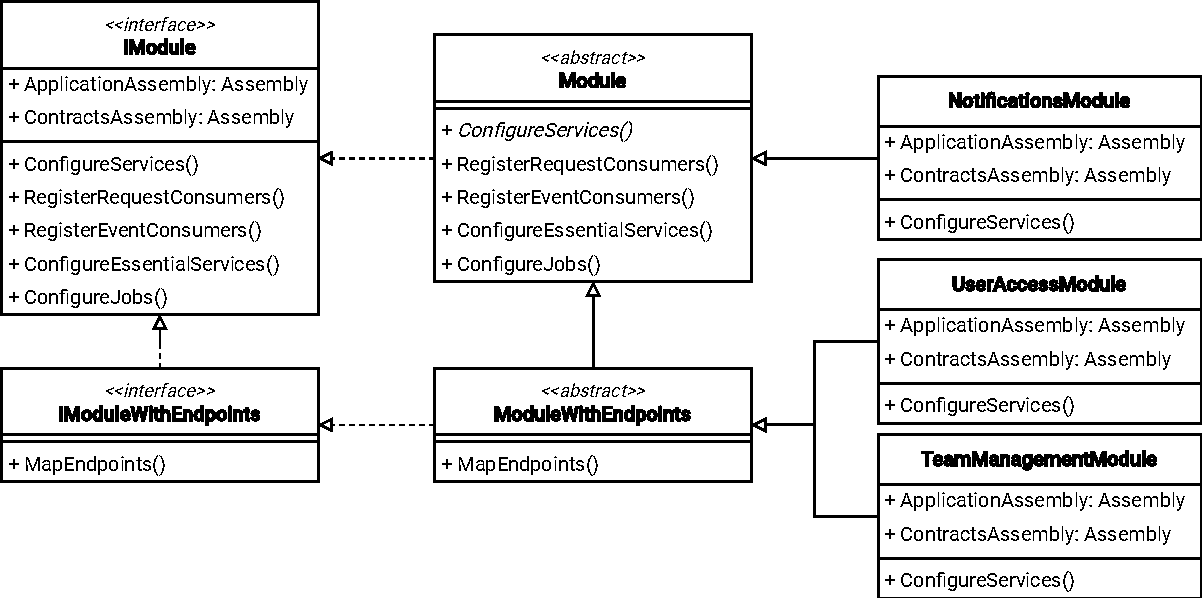
\includegraphics[width=\textwidth]{figures/cd-modules.pdf}
    \caption{A class diagram representing the module abstraction, required assembly properties serve to automatically register commands, queries, and event handlers. The~diagram intentionally excludes parameters, data types, and some other properties and methods on order to better outline the abstraction design. The diagram also does not contain generics (f.e. notifications module inheriting \texttt{Module<NotificationsModuleId, NotificationsDbContext>}) that is needed by the \texttt{Module} base class to properly register essesntial services.}
    \label{fig:mm_cd_modules}
\end{figure}

Some services (called \textit{shared services} for the purpose of this thesis) need a different implementation per module, but with exactly the same logic. So the service can, for example, do the same but with a different database context (e.g. unit of work). The challenge is to~provide the correct service implementations to~the~respective modules.

Since the DI provider integrated in frameworks on the .NET platform does not support modular dependency injection\footnote{Microsoft recommends using 3rd party DI providers, such as \textbf{Autofac} (\url{https://autofac.org/}).}, it is necessary to work around this so that each module is injected with the corresponding \textit{shared service} implementation:

\begin{itemize}
    \item One solution is to register \textit{shared services} as a \textbf{keyed service} and retrieve service implementation from DI container by type and key.
    
    e.g. \texttt{ctor([FromKeyedServices(\textquotedbl userAccessModule\textquotedbl)] IUnitOfWork instance)}
    
    \item The more convenient approach is to take advantage of generics and mark service implementations with class representing \textbf{module id} (in contracts layer) which is passed to the module base class and leveraged to automatically register \textit{shared services} with it.

    e.g. \texttt{ctor(IUnitOfWork<UserAccessModuleId> instance)}
\end{itemize}

\subsubsection{Inbox and Integration Events}
While publishing and processing domain events works the same as in the Clean Architecture solution (see \ref{dev:ca:infra}), the modular monolith design adds to the complexity of integration events as the integration event, in addition to the asynchronous side effects (e.g. sending an email), also represents state changes that need to be propagated over the message bus to~multiple modules, therefore introducing necessity for an outbox and an inbox per module. 

Furthermore, implementing multiple outboxes and inboxes with MassTransit poses some issues (see section \ref{problem:multiple} about encountered problems).

Integration event lifetime:
\begin{enumerate}
    \item Integration event is stored as an outbox message in database within a single transaction (covering all request changes) using the \texttt{IntegrationEventPublisher} (inside the domain event handler/domain service).

    \item In the background processing iteration, the outbox consumer of a given module takes X outbox messages, converts them back to integration events, and publishes them to~the~RabbitMQ bus using the MassTransit API.

    If the publishing is successful, the message is removed from the outbox.

    \item The MassTransit consumer registered to a given integration event receives a message with the event and stores this event as an inbox message.

    \item In the background processing iteration, the inbox consumer of a given module takes Y inbox messages, deserializes them into integration events, and invokes concrete integration event handlers for a given module.

    If the handling is successful, the message is removed from the inbox. 
\end{enumerate}

One of the difficulties in event-driven systems is the possibility of receiving the same message multiple times, so the handlers should be idempotent if possible; the module can also maintain a buffer of recent events to detect duplicates (not used in the solution).

Another problem originates from the possibility of handling events out of order, especially when duplicates may occur as well. The basic idea is to keep failing until the data required for correct handling arrives (some handlers may require more granular error handling).

\begin{figure} [H]
    \centering
    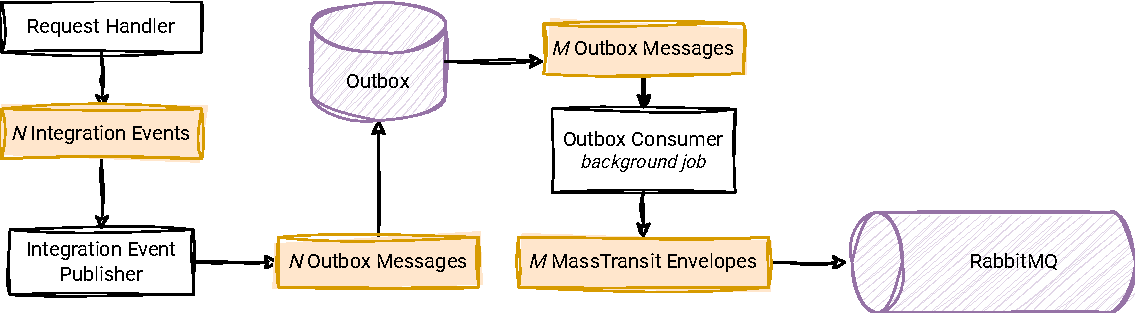
\includegraphics[width=\textwidth]{figures/mm-produce-pipeline.pdf}
    \caption{Detailed diagram of a pipeline for reliable asynchronous publishing of integration events to the event bus. This entire pipeline is executed within a single module.}
    \label{fig:mm_produce_pipeline}
\end{figure}

\begin{figure} [H]
    \centering
    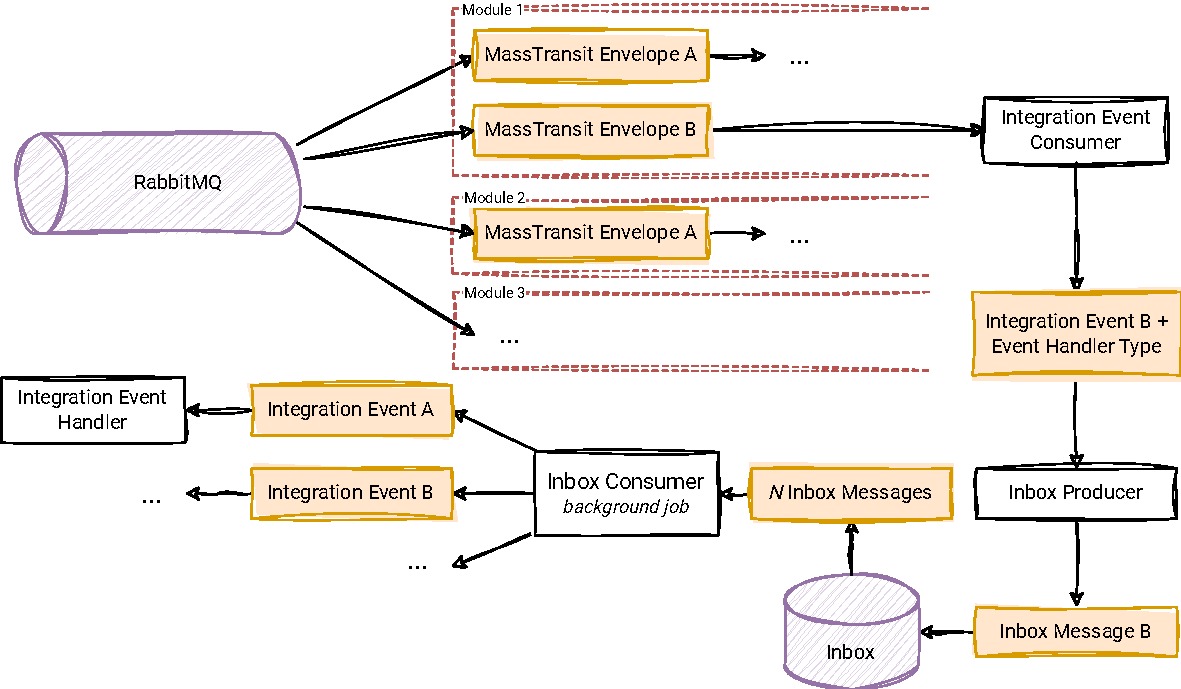
\includegraphics[width=\textwidth]{figures/mm-consume-pipeline.pdf}
    \caption{Detailed diagram of a pipeline for reliable asynchronous consumption of integration events from the event bus. As illustrated, a single event can be send to multiple modules. In case a module has more consumers for a single event, each will produce its own inbox message with a dedicated event handler.}
    \label{fig:mm_consume_pipeline}
\end{figure}

Note that event handlers must not implement more than 1 atomic functionality (side effect/transaction). This is because the execution of one functionality can be successful and if the event handling is repeated due to the failure of others, the successful one would be repeated as well (i.e. sending 1 email multiple times). The solution does register a separate inbox message per integration event consumption for flawless multi-handling of a single event within a module (as illustrated in figure \ref{fig:mm_consume_pipeline}).

\newpage
\subsection{Invite unregistered user workflow example}
\vspace{-10pt}
\begin{figure} [H]
    \centering
    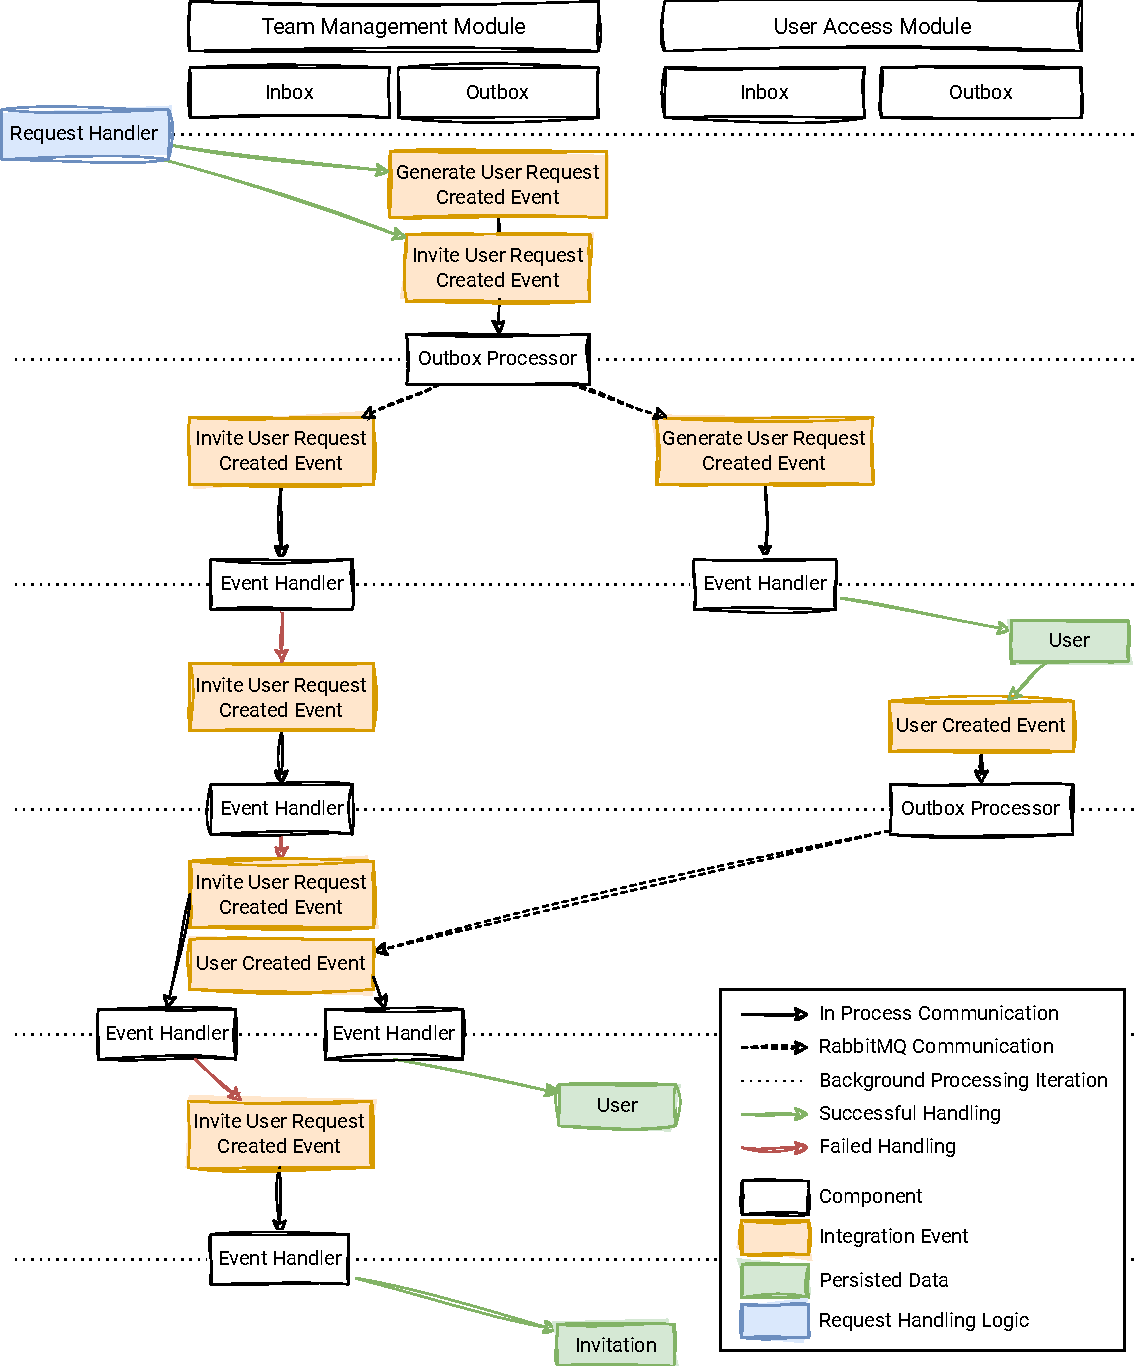
\includegraphics[width=0.99\textwidth]{figures/mm-workflow.pdf}
    \caption{Simplified diagram illustrating the communication within and between modules to create a user invitation. Note that the handling of the \textit{invite user request created event} failed several times until the module eventually obtained the necessary data and arrived to~a~consistent state for creating the invitation. In contrast to the workflow from the Clean Architecture solution (figure \ref{fig:ca_workflow}), the system cannot immediately return \texttt{201 Created} because the system is eventual consistent, but rather returns \texttt{202 Accepted} indicating that the API request has been successfully processed. The diagram also omits integration events sent to the notification module caused by the user and invitation creation.}
    \label{fig:mm_workflow}
\end{figure}

\section{Frontend app}
\label{dev:frontend}
The entire frontend solution is available online as a repository on GitHub:

\url{https://github.com/skrasekmichael/ModularInformationSystemFrontend}

\subsection{Implementation}
The frontend application is implemented using the \textbf{Blazor}\footnote{\url{https://learn.microsoft.com/en-us/aspnet/core/blazor/}} fronted framework with a~separate hosting server from the backend and with \texttt{InteractiveAuto} render mode (see below).

Since the Blazor application logic can run both on the server and in the client browser, it is necessary to keep the authentication/authorization state accessible from both modes, that is, by storing the JWT token in a cookie.

Application UI is built using the \textbf{Fluent UI}\footnote{\url{https://github.com/microsoft/fluentui-blazor}} components library for Blazor by Microsoft, utilizing the fluent design system and fluent icons.

To notify and propagate data and UI changes between components across the application, a \textbf{mediator pattern} with a runtime message subscription capabilities is used; the MVVM Community Toolkit library implements such a mediator called \textbf{messenger}\footnote{\url{https://learn.microsoft.com/en-us/dotnet/communitytoolkit/mvvm/messenger}} (application uses only the \texttt{WeakReferenceMessenger}).

Project structure: \vspace{6pt}

\dirtree{%
.1 TeamUp/\DTcomment{frontend repository}.
.2 src/.
.3 TeamUp/\DTcomment{Blazor hosting server assembly}.
.4 Components/\DTcomment{server side components}.
.4 wwwroot/\DTcomment{static files}.
.4 \dots.
.3 TeamUp.Client\DTcomment{Blazor client assembly}.
.4 AnonymousPages/\DTcomment{pages accessible without login}.
.4 Components/\DTcomment{components}.
.4 Layout/\DTcomment{application layouts}.
.4 Pages/\DTcomment{pages requiring logged-in user}.
.4 \dots.
.3 TeamUp.Contracts\DTcomment{API contracts}.
.3 TeamUp.DAL\DTcomment{data access components}.
.4 Api/\DTcomment{API client}.
.4 Cache/\DTcomment{caching services}.
.4 Messages/\DTcomment{mediator messages}.
.4 Services/\DTcomment{data access services}.
.4 \dots.
.2 TeamUp.sln.
.2 \dots.
}

\newpage
\subsubsection{Blazor}
ASP.NET Core \textbf{Blazor} is a .NET frontend web framework for building full-stack interactive web applications and as such is the .NET flagship for frontend development.

Blazor provides a single model for both server side and client side interactivity written in~C\# with component-based architecture and several render modes:
\begin{itemize}
    \item \textbf{Static SSR} where server renders non-interactive HTML content. This is also used for fast pre-rendering of content when using interactive modes.

    \item \textbf{Interactive SSR} (also used in \textit{Blazor Server}) where client has open SignalR connection (Web Socket) to the server and interactive handling (button click, \dots) is executed on the server side together with re-rendering of affected components.

    \item \textbf{Interactive CSR} (also used in \textit{Blazor WASM}) relies on .NET runtime build with Web Assembly (WASM) that is downloaded with the application, all code is then executed in the browser. This provides full access to functionality of the browser and interop with Java Script (DOM, local storage, etc.).
\end{itemize}

The main advantage of Blazor is the ability to combine interactive SSR and CSR together:

Starting with .NET 8.0, the first time web application is accessed, the interactivity starts on the server, and once the .NET WASM runtime and application are downloaded, the~application switches to the client-side interactivity, eliminating the main drawback of Blazor WASM -- the long download time. This render mode is called \texttt{InteractiveAuto}, marking that system automatically decides which render mode to use.

The framework also allows to specify the rendering mode per component, but it is not allowed to have an application with interactive SSR and CSR at the same time.

\subsubsection{API Client}
There are several key aspects to the API client integration with the backend:

\begin{itemize}
    \item \textbf{CORS} -- server CORS settings allow API calls from the Blazor application.

    \item \textbf{Token Injection} -- the API client automatically injects JWT tokens into API calls when user is logged in.

    \item \textbf{Error Handling} -- since the backend API returns a problem detail response (or validation problem details) in case of errors, the API client can easily parse the responses and act accordingly. If the API returns an unauthorized response code, the API client logs the user out since the unauthorized code indicates token expiration.

    \item API calls vary based on interactive modes:
    \begin{itemize}
        \item SSR: Calls originate from the frontend server to the backend server API.
        \item CSR: Calls are made directly from the browser to the backend server API.
    \end{itemize}
\end{itemize}

\subsubsection{Caching}
Client-side caching can eliminate many network calls and therefore has the potential to~improve performance more than the server-side caching, in addition to using user resources. However, the client-side caching introduces bigger chance for a user to work on invalid data, since updates from other users cannot invalidate the client-side cache,

The \textbf{cache-aside pattern} is implemented using the browser's key-value local storage (see figure \ref{fig:cache}), working as follows:

\begin{enumerate}
    \item UI requests data (API contracts) via a DAL service.

    \item DAL service calls to the \textit{Cache Façade} with the following parameters: cache key, API fallback endpoint, and cache lifetime. DAL services have methods for all GET endpoints allowing to specify the cache lifetime per contract/endpoint.

    \item The \textit{Cache Façade} data lookup:
    \begin{itemize}
        \item On cache hit -- validates cache records lifetime expiration (cache miss on expired) and returns cached data.

        \item On cache miss -- fetches data from the fallback API endpoint, caches them and returns them to the DAL service.
    \end{itemize}
\end{enumerate}

One problem arises when a user logs out (intentionally or by token expiration) and the data remains in the local storage. Hence, if another user logs in, the application displays incorrect data and the user has read access to someone else's data until the token expires. This is resolved in the application by also caching the \textit{cache owner}, and clearing the cache if the~logged-in user differs from the \textit{cache owner}. This allows reuse of the cached data when re-logging in, however, the data is still accessible before logging in and the application provides a \textit{clear cache} button for multi-user-single-browser situations (presumably unusual).

\begin{figure} [H]
    \centering
    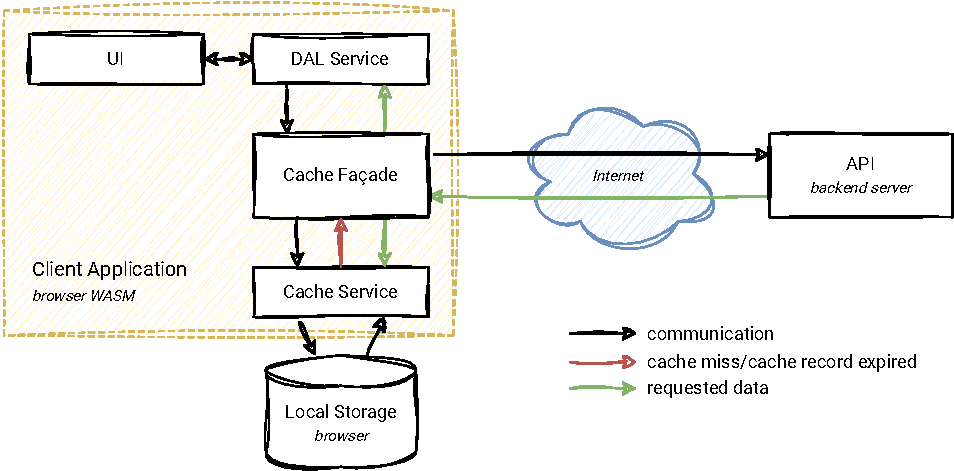
\includegraphics[width=\textwidth]{figures/cache.pdf}
    \caption{A diagram showing the implementation of the cache-aside pattern with a~browner local storage serving as a cache storage and an API call as a fallback in case of~a~cache miss. Note that the data is cached after each GET request.}
    \label{fig:cache}
\end{figure}

Client-side caching in the Blazor applications is challenging due to the possibility of running the code both on the client-side and server-side, introducing problem to uniformly access a cache. That is why the diagram in figure \ref{fig:cache} has additional \textit{Cache Service} layer around the local storage to provide different caching service on server-side and client-side.

Server-side rendering modes have following properties:
\begin{itemize}
    \item In static SSR mode, the application does not have access to the browser resources and the only caching option is to use server-side caching solution or some sort of HTTP cache (both are undesirable due to incompatibility with the client-side cache).

    \item In interactive SSR mode, the application has access to Java Script interop after a~page rendering, resulting in initially calling the API and later in cache hit/miss.
\end{itemize}

Possible solutions:
\begin{itemize}
    \item One solution is to not use cache on the server, and always call API to retrieve data.
    
    \item Another solution migth be to implement different caching mechanism on the server (i.e. in-memory cache) and lose all cached data when switching to CSR. In such case, it may be preferable to implement a robust caching mechanism on the backend server and always call the API to retrieve data in the Blazor application.

    \item The solution used in the application is to not use the cache when the local storage is unavailable (static SSR, early interactive SSR), but otherwise to use it even though cached data is transferred from the client to the server, processed there, and transferred back to the client, because this approach maintains a single consistent cache storage and the application can use these cached entries when switching to CSR mode.
\end{itemize}

\begin{figure} [H]
    \centering
    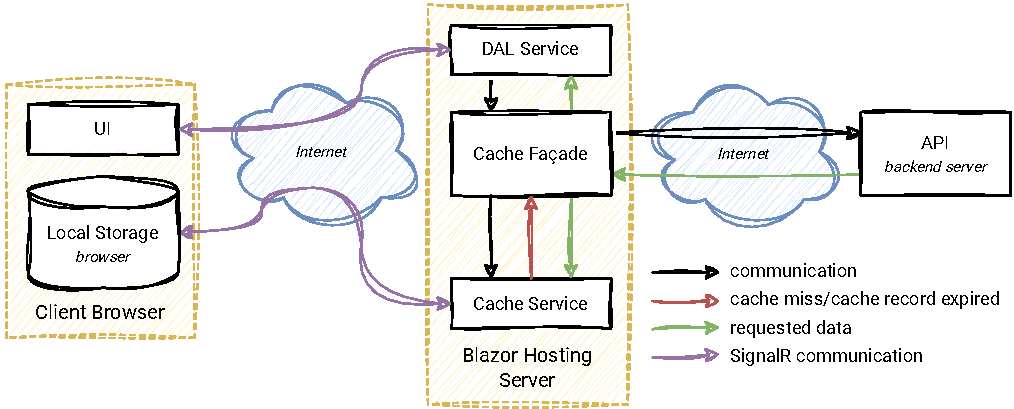
\includegraphics[width=\textwidth]{figures/server-cache.pdf}
    \caption{A diagram showing the implementation of the cache-aside pattern when the~application is running in the interactive server mode. Note that the~Blazor hosting server can be positioned either close to the server (e.g. on the same machine) or distributed at~the~cloud edge (close to the client), reducing communication penalty either to the client or to the API, respectively.}
    \label{fig:server-cache}
\end{figure}

\newpage
\section{Interesting parts}
\label{dev:interesting}
This section covers topics and parts of the solutions and development process that are not the primary focus of this thesis, but may still be of interest to the reader.

\subsection{Encountered problems}
\label{dev:problems}
While developing backend solutions, I encountered problems regarding technologies and design choices that were challenging or interesting to solve. 

\subsubsection{Inbox Starvation}
The inbox (outbox) starvation is a term coined by me\footnote{The analogy is that the system is starving for new events.} to refer to a problem where the inbox contains a sufficient number of integration events that continuously fail to be consumed, and the entire consumption gets stalled because the background service keeps processing the same failing events to preserve the order of events.

This can be addressed by continually increasing the delay between the consumption of failed events, by deleting/skipping events that have failed multiple times, or by a combination of~both; the solution heavily depends on the concrete logic of integration event handlers.

Some integration event handlers may even count on repeated failures due to eventual consistency (waiting for data that will be eventually available, see for example workflow diagram in figure \ref{fig:mm_workflow}), this leads to a reduction of effectively consumed events per iteration or even to temporary inbox starvation until repeatedly failing events are successfully handled.

In the Modular Monolith solution, the outbox starvation is not a problem because the~inability to consume outbox messages indicates that the event bus is down (low probability, the application should not work in this case) or that there is a bug.

The Clean Architecture solution has the same problem with outbox starvation, because the outbox and inbox are merged together. Since the system uses integration events only for sending emails, failing to send should only delay the processing of other emails, but there is a possibility of a tailored attack targeting the inbox that could lead to starvation. Moreover, the inbox starvation problem should be taken into account when adding more asynchronous side effects to the system.

Both solutions implements measures of tracking the number of times a message failed to be processed and continuously postponing the next processing of a given message. This also potentially changes timings and duration of certain workflows that are based on waiting in~the~inbox for an eventually consistent state (for example workflow diagram in figure \ref{fig:mm_workflow} might fail fewer times but take longer to complete.).

Note that designing strategies (postponing timings, growth rate, etc.) for handling repeated message processing failures is a complex task and bad error handling strategy might crash the entire system. Continuous monitoring and possible strategy adjustments are a good start to address such problem. In addition, it would be possible to split the inbox/outbox messages into groups with different error handling strategies or even specify a strategy per~integration event handler as a more granular approach.

\newpage
\subsubsection{Multiple outboxes with MassTransit}
\label{problem:multiple}
MassTransit is an excellent framework for building distributed systems (e.g. microservices) with the ability to configure an outbox pattern, however, it is limited to one database context and one outbox per application, which leads to limited usability in a modular monolith applications.

Explored solutions:
\begin{itemize}
    \item Different communication framework, for example NServiceBus, might solve the problem, but a brief study of the documentation have not confirmed this ability (it is not the most requested feature) and migrating to/learning a new framework is expansive.

    \item A single outbox for the entire modular monolith in a separate database schema and transactions covering the module schema and the outbox schema is a possible solution, but it moves away from the modular (``microservice-like'') approach and may introduce unintuitive issues (odd behaviour during tests).

    \item Mimicking microservices in the context of dependency injection (looking like a single executable) using a modular DI provider (e.g. Autofac) so that each module registers its own services required by MassTransit, including the database context for~the~outbox, etc. This solution does not imply success, as there might still be issues with registration of background services, plus switching DI providers is both knowledge and resource intensive and the new provider may be incompatible with other libraries.

    \item Solution used in this thesis: custom implementation of inbox and outbox, and integrating them with MassTransit as a transport layer, that includes:
    \begin{itemize}
        \item Definition/configuration of outbox and inbox messages, including db migration.
        \item Implementation of background services for consuming the inbox and outbox (2 background services per module).
        \item Wiring MassTransit consumers to respective module inbox.
    \end{itemize}

    This allows complete control over how the system should work, inducing inbox starvation, but introduces extra work and complexity. Custom solution might also be full of bugs, inefficiencies, and bad design choices.
\end{itemize}

Implementing the outbox pattern for request-response communication (commands/queries) is unnecessary because the failure is propagated back to the request producer, which is:
\begin{itemize}
    \item[A)] Inside the integration event handler (the main use case), when the integration event handler fails and the inbox pattern for integration events kicks in.
    
    \item[B)] Inside the request processing logic, in which case the request fails and the error message is delivered back to the API client (the user) who resolves the error accordingly.
\end{itemize}

Alternatively, MassTransit offers the option to use In-Memory Outbox, which supposedly ensures eventual consistency in the event of a database or a message transfer failure.\footnote{see \url{https://masstransit.io/documentation/patterns/in-memory-outbox}}

\subsubsection{Value Objects in Entity Framework Core}
The Ef Core supports multiple ways of persisting and dealing with value types:

\begin{itemize}
    \item The EF Core has the ability to provide custom \textbf{value conversions} to serialize types into a single column, which is most probably not a solution for a value object, because the system loses the ability to effectively use object properties in queries. 

    This option might be useful for single-valued objects (i.e. strongly typed id) or for~types where querying over nested properties does not make sense or will not be used.
    
    For example, the query capability over the \texttt{R} part of  the \texttt{RGB} value seems pointless, however, the ability to select only records where \texttt{money} value is in certain \texttt{currency} (nested property of the \texttt{money} value object) may be desirable.
    
    \item Since version 2.0, the EF Core provides the \textbf{Owned Entity Type} capability, as~described in the EF Cores documentation \cite{ms:efcore:owned_types}; entities use implicit keys, meaning that a shadow id is created so that the EF Core is able to keep track of them, which contradicts the idea of a value object.
    
    \item As of version 8.0, the EF Core introduces the \textbf{Complex Type} option. An official blog post about the version \cite{ms:blog:complex_types} highlights 2 main advantages over owned types:
    \begin{itemize}
        \item Complex types are not identified or tracked by key value.
        \item Complex types can be both \textbf{.NET value types} (structs) and reference types.
    \end{itemize}
\end{itemize}

The solutions use value converters for strongly typed ids and for password type (composed from \textit{seed} and \textit{hash} values) without problems.

Unfortunately, the use of a complex type (\texttt{EventReply} composed from \textit{reply type} and \textit{message}) caused a problem when using \texttt{GROUP BY} over the \textit{reply type} property: 

The EF Core was throwing an exception that it was unable to build an SQL query and wanted to fetch all data from the database and perform grouping in-memory.

Possible solutions:
\begin{itemize}
    \item Solution used in this thesis: removing the value object from the entity property and using it only as contract in methods with manual mappings to entities properties.
    
    \item Another solution could be to use EF Core's ability to execute RAW SQL queries and build the SQL query manually, since the database has the actual properties available in separate columns for available grouping.
    
    \item Probably the best solution would be to embrace the CQRS pattern and use a more lightweight approach for querying the data, like a direct SQL client or preferably a~micro ORM framework, which would most likely lead to better performance.
\end{itemize}

Although attempts to reproduce this error have been made, they have not been succesful, and using \texttt{GROUP BY} in similar situations resulted in the correct and expected behaviour.

\subsection{Result Pattern and Railway Oriented Programming}
\label{interesting:rp_rop}
The entire application solution leverages the result pattern for error handling, and most of~the~business logic takes advantage of railway-oriented programming to provide cleaner and easier-to-understand code. 

To avoid code duplicity between the clean architecture solution and the modular monolith solution, as well as the possibility of future usage, a decision to publish the result pattern implementation and railway-oriented extension methods as separate nuget packages\footnote{\url{https://github.com/skrasekmichael/RailwayResult}} has been made. 

\subsubsection{Result Pattern}
The result pattern, result object or operation result, is a way to control error handling in~an~application without the use of exceptions, as the exception handling (try-catch blocks) branches the code, thereby reducing code clarity and obscuring the underlying business logic. Another drawback of using exceptions might be the performance, as throwing an~exception is an expensive operation. On the other hand, the ability to trace the exact location of the thrown exceptions in code (stack trace) brings superior debugging experience.

The result object is a \textbf{discriminated union} of \textbf{success state} and \textbf{failure state}, where the operation (method) returns a success result if no error occurred, and a failure result if some sort of error/exception case occurred (validation error, IO error and so on). The~result object also carries the returned operation value in case of a success state, or error details (error code, message) in case of a failure state.

In the context of web applications providing REST APIs, the result object can be mapped to the corresponding http response -- Ok/Created/Accepted/\dots~for a successful result, and in the case of a failed result, the error can be mapped to the \textbf{problem details}\footnote{\url{https://datatracker.ietf.org/doc/html/rfc7807}} with appropriate details including status code (BadRequest/NotFound/Conflict/\dots) and other.

Predefined error types for result pattern:
\begin{itemize}
    \item \texttt{AuthenticationError} -- authentication failure (invalid credentials).
    \item \texttt{AuthorizationError} -- forbidden to perform operation/forbidden access.
    \item \texttt{ValidationError} -- invalid input request parameter.
    \item \texttt{NotFoundError} -- domain object not found.
    \item \texttt{ConflictError} -- existing conflicting domain object, concurrency conflict, etc.
    \item \texttt{DomainError} -- broken business rule that does not fit into other errors types.
    \item \texttt{InternalError} -- unexpected behaviour (uncaught exception, bug, etc.). 
\end{itemize}

Using the implicit operators feature in C-Sharp, the boilerplate for creating the result object can be removed, and therefore the error types and returning values implicitly create a new result object (see example in figure \ref{fig:set-member-role}).

\begin{figure} [H]
    \centering
    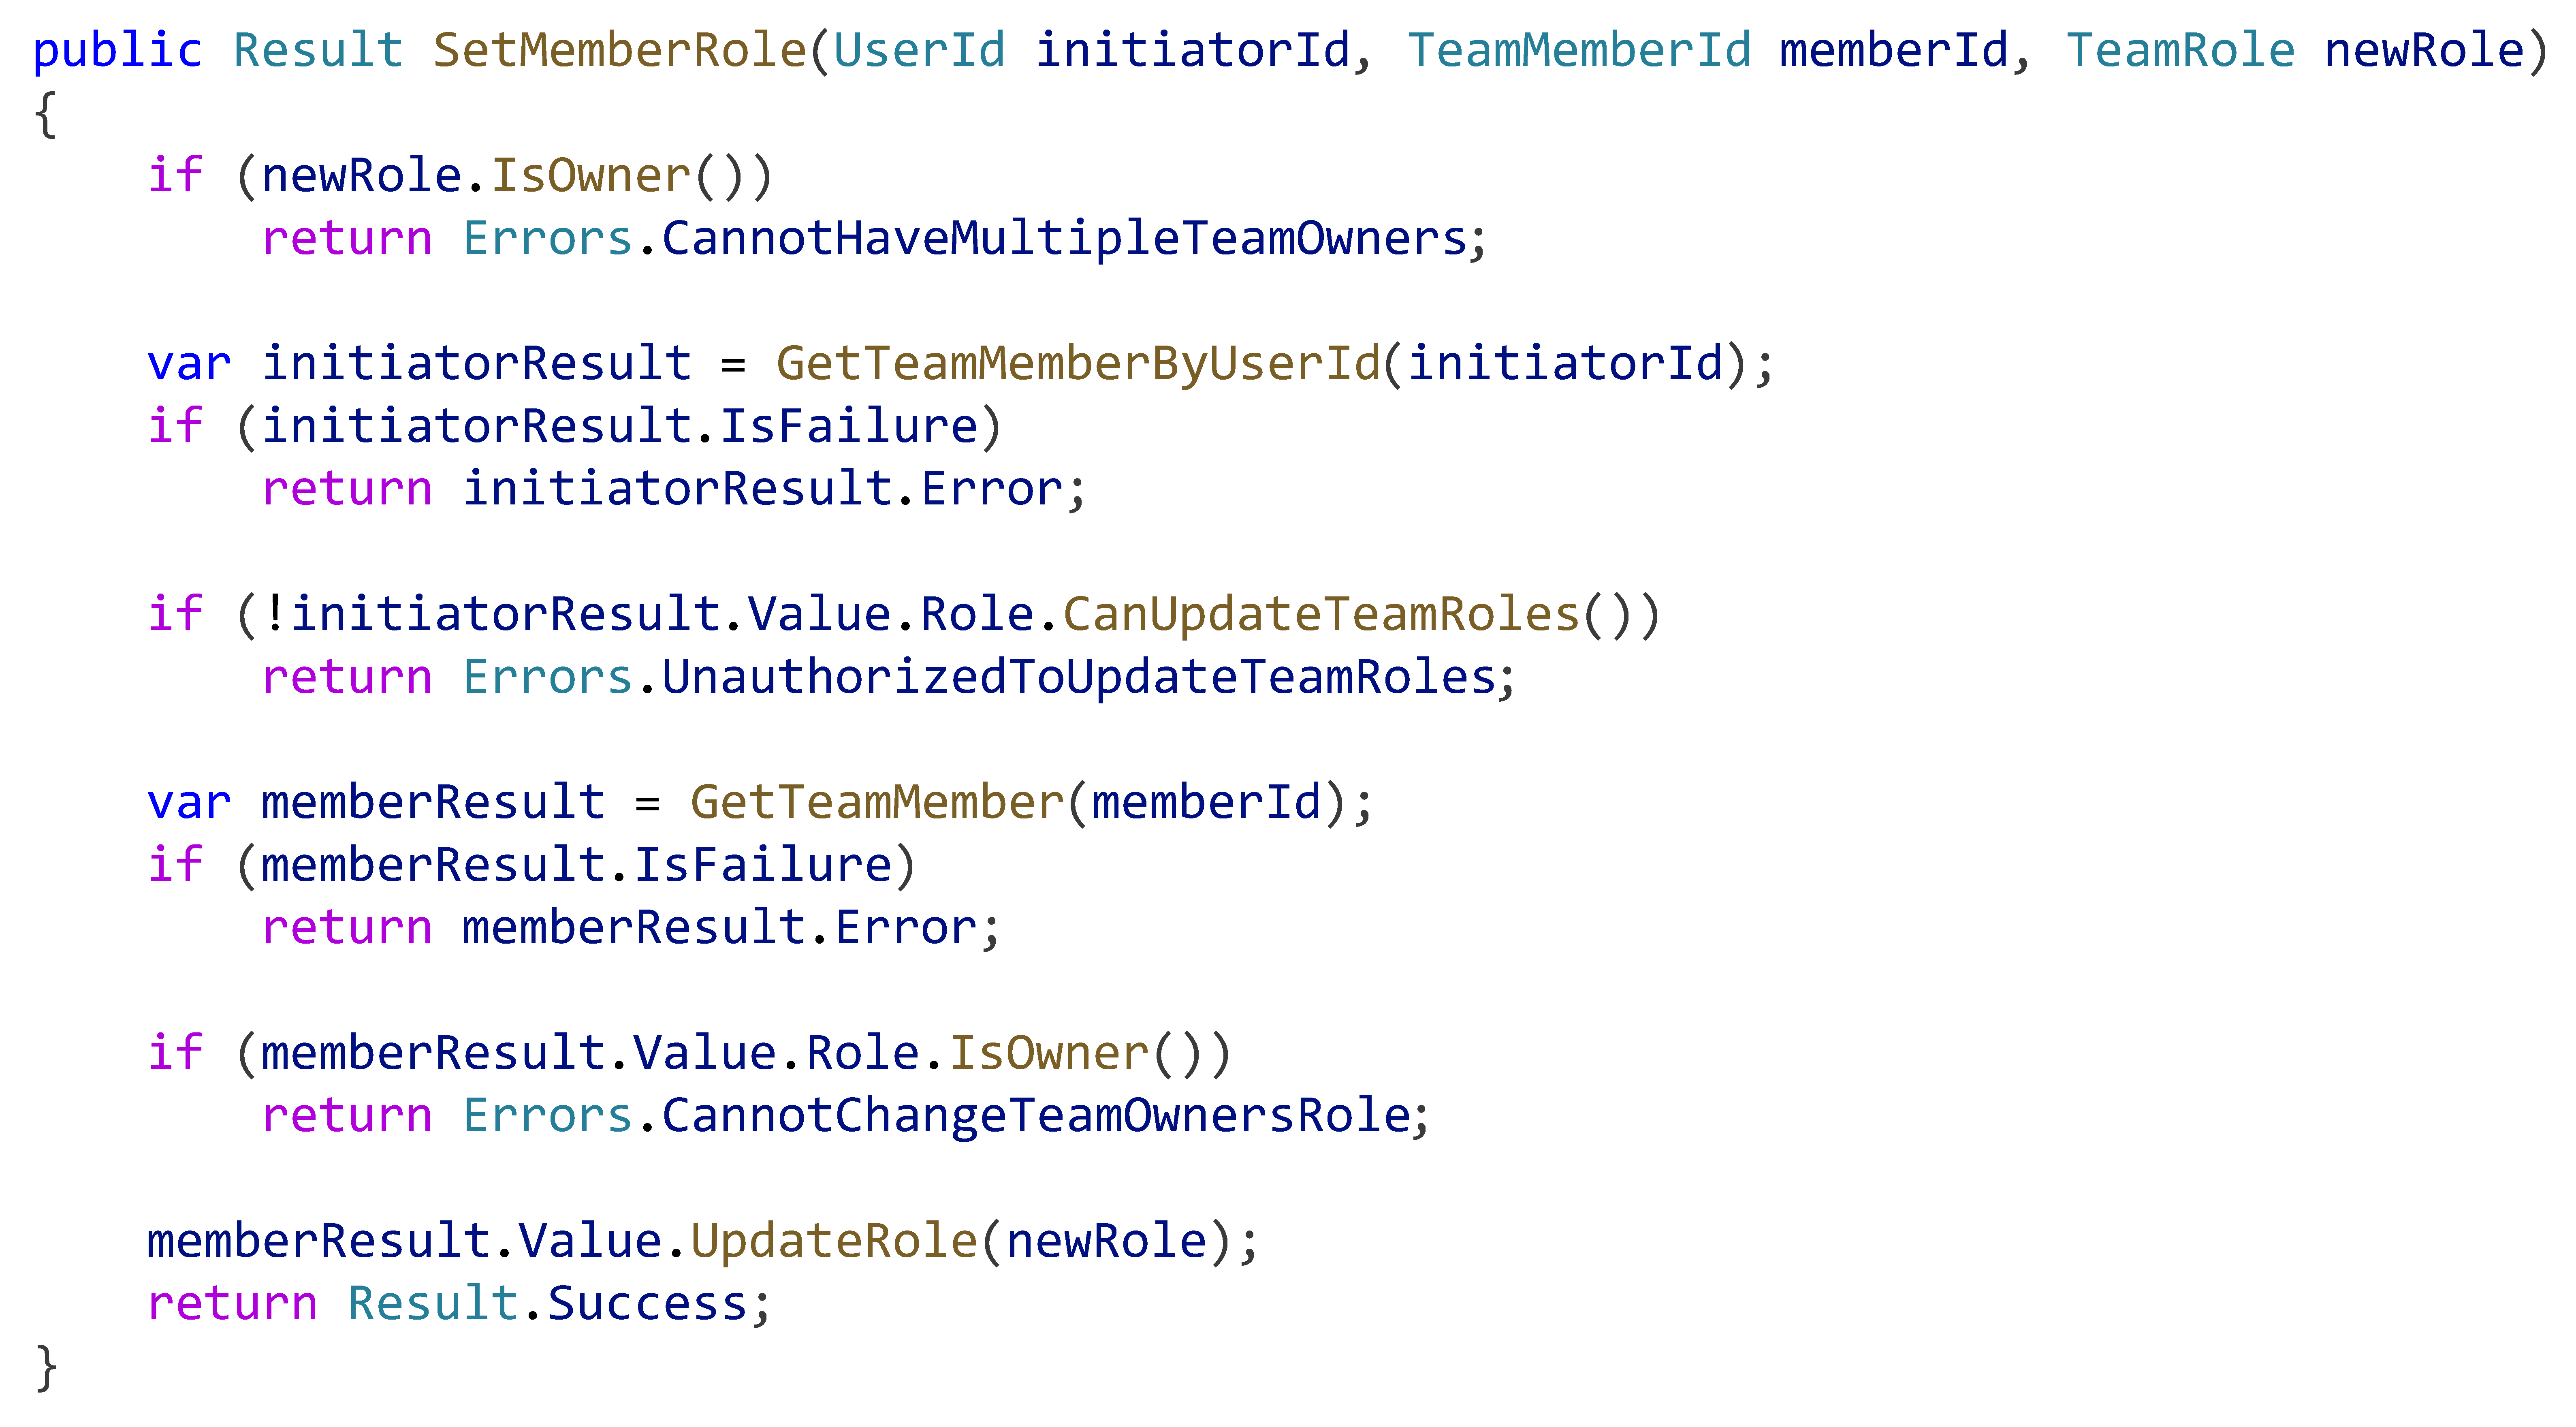
\includegraphics[width=\textwidth]{figures/set-member-role.pdf}
    \caption{Code example of using the result pattern in the \texttt{SetMemberRole} method of the team aggregate, where \texttt{Errors} is a static class containing predefined errors.}
    \label{fig:set-member-role}
\end{figure}

\subsubsection{Railway Oriented Programming}
Railway-oriented programming (ROP) is an approach to error handling in functional programming. The name comes from an analogy presented by Scott Wlaschin at the NDC London 2014 conference \cite{scott_wlaschin:rop}, which presents the flow through a program as a railway with 2 tracks, a success track and a failure track, and for each operation/method the state can switch to failure track if an error occurs (see figure \ref{fig:rop}).

\begin{figure} [H]
    \centering
    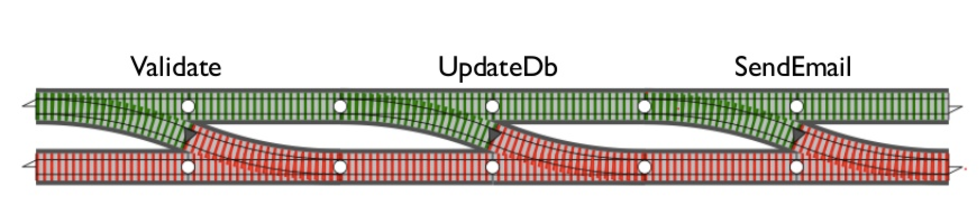
\includegraphics[width=\textwidth]{figures/rop.png}
    \caption{An example of a program flow where each function can throw an error and switch the state to the failure track, thus not invoke the following functions. This example it taken from the presentation slides from the \cite{scott_wlaschin:rop} blog post.}
    \label{fig:rop}
\end{figure}

This is a natural extension of the result pattern as the result object representa a state on the~railway (either success or error) and the methods returning result pattern act as switches on the program railway.

However, in classical programming using the result pattern, the result object is only returned and not taken as an input in the methods, and it is undesirable for~each function to~take the result object as a parameter and have all the original parameters as a nested value of~the~result object. The solution is to introduce functional extension methods on~the~result object that always check the state of~the~result object and then apply the logic wrapped in~the passed parameter.

Main extension methods:
\begin{itemize}
    \item \texttt{.Ensure(predicate, error)} -- validates whether the value meets the condition on the success track, or returns the \texttt{error} (switches to failure track).
    \item \texttt{.Then(mappingFunction)} -- maps the value of the result object on the success track to a new value (also called .Map). If the mapping function returns a failure result, it returns its error (switches to failure track).
    \item \texttt{.Tap(function)} -- invokes a function (side effect) on the success track but does not change the type of the result object. If the mapping function returns a failure result, it returns its error (switches to failure track).
    \item \texttt{.And(mappingFunction)} -- generates another value using the mapping function on the success track and encapsulates it with the initial value inside the result object.
\end{itemize}

To fully utilize ROP in the .NET, the asynchronous variants of the methods need to be implemented to perform non-blocking operations.

\begin{figure} [H]
    \centering
    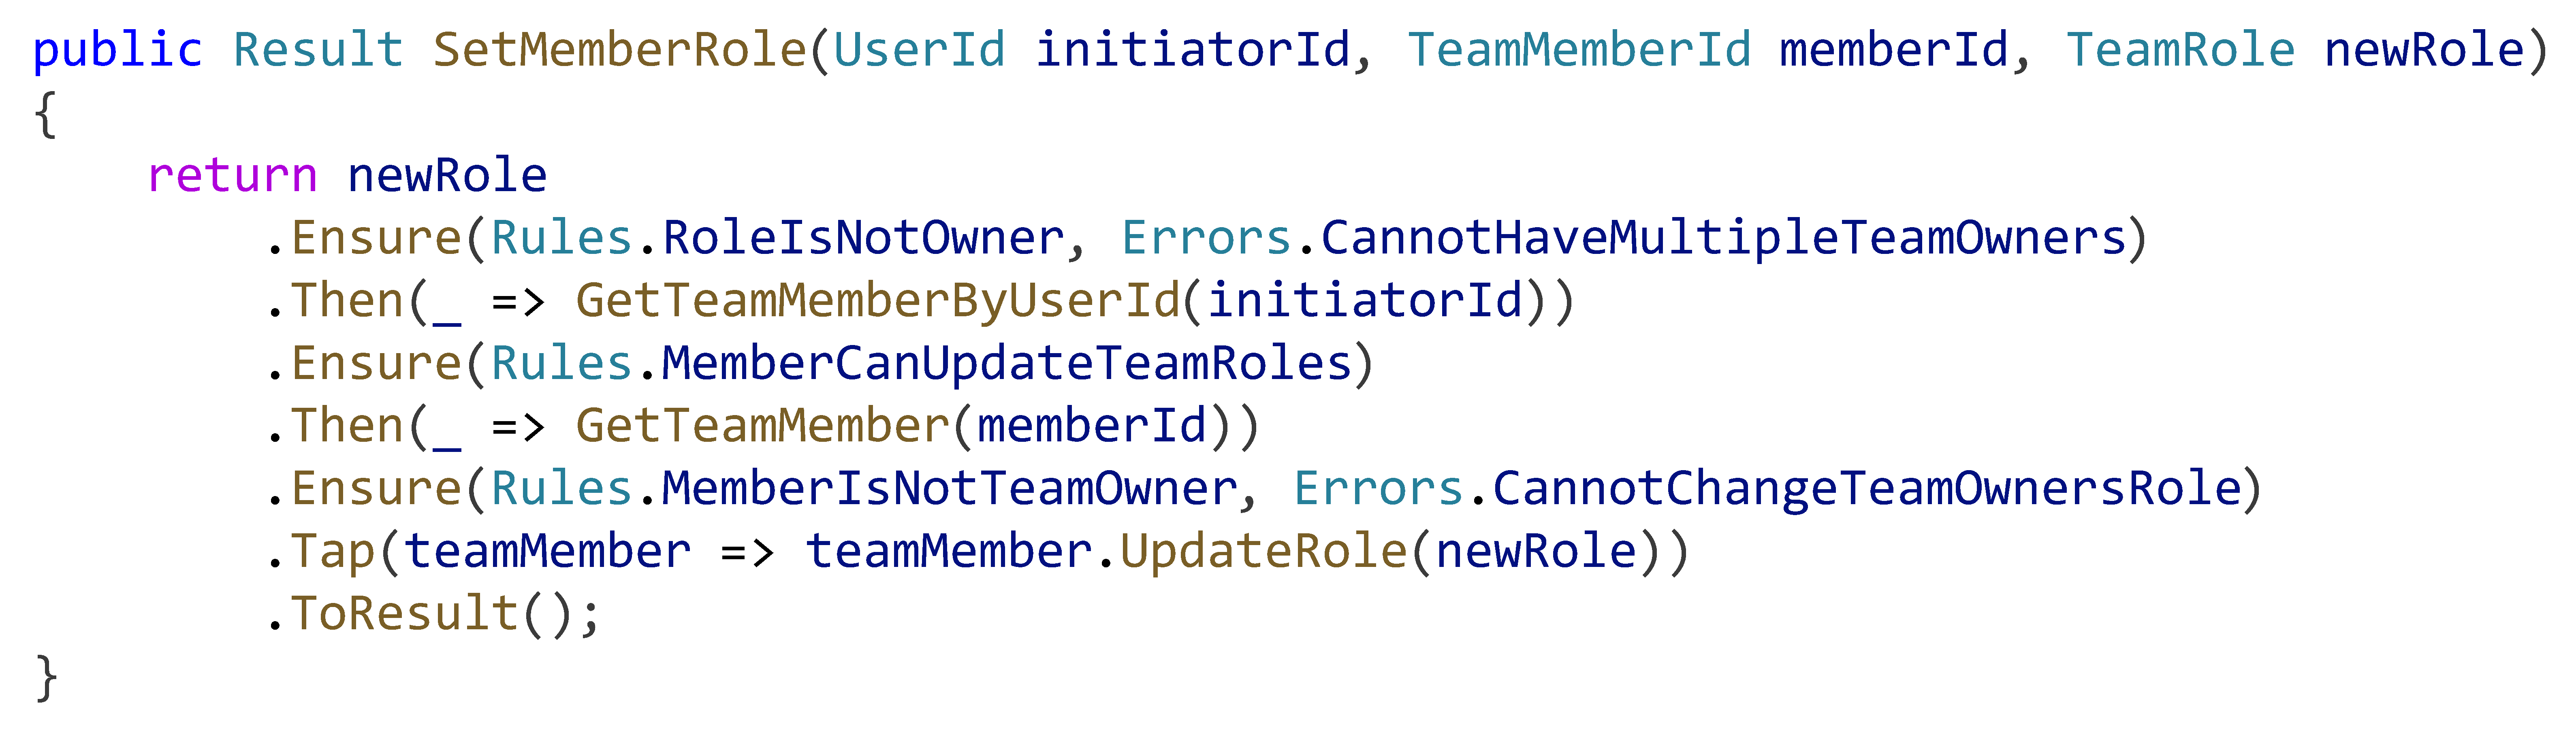
\includegraphics[width=\textwidth]{figures/set-member-role-rop.pdf}
    \caption{Code example of the same \texttt{SetMemberRole} method in the team aggregate as~in~figure \ref{fig:set-member-role}, but utilizing railway-oriented programming. \texttt{Rules} is a static class with predefined rules, that is, predicates and predicates with preassigned appropriate errors. The \texttt{.ToResult()} method drops the wrapped value and returns plain result object. This is a copy of the exact code used in the solution source code.}
    \label{fig:set-member-role-rop}
\end{figure}

Even though the ROP results in shorter and (hopefully) cleaner code, there are a few drawbacks mentioned by Scott Wlaschin \cite{scott_wlaschin:norop}.

The main disadvantage of railway-oriented programming is \textbf{performance}, since when using ROP the code loses the ability to return early from a function (aka fail fast), thus introducing the necessity to go through the entire railway statement even if an error occurs in the first method.

Furthermore each method of railway statement has an overhead of at least 1 track check and an allocation of data (parameters and possible new result), and even more for asynchronous variants as the methods bootstrap a state machine and allocate more data.

\subsection{Database Concurrency Conflicts}
\label{dev:conccurency_conflicts}
The EF Core does not support multiple parallel operations running on the same database context, so in ASP.NET Core applications, contexts are scoped per http request, meaning that there may be 2 (or more) concurrent modifying requests to the same record without the contexts knowing and addressing this conflict.

If a concurrent request modifies the same record at the time of checking the business rules (after fetching data from the database but before committing changes), the initial request transaction will conclude with possibly incorrectly evaluated business rules or update the~record to a new value calculated from the initially fetched data, resulting in data loss and leaving the database in an inconsistent state. This phenomenon is also known as~a~\textbf{race condition}.

An example of data loss when updating account points:

\texttt{req A: get points -> pointsA = 100\\
req B: get points -> pointsB = 100\\
req B: set points -> points = pointsB - 50 = 50 -> commit 50\\
req A: set points -> points = pointsA + 50 = 150 -> commit \textcolor{red}{150}\\
-> }as a result, request B loses its effect.

Inconsistent state example when reserving tickets:

\texttt{req A: get number of available spots -> availableA = 3\\
req B: get number of available spots -> availableB = 3\\
req A: reserve 2 tickets -> availableA - 2 >= 0 -> commit reservationA\\
req B: reserve 3 tickets -> availableB - 3 >= 0 -> commit \textcolor{red}{reservationB}\\
-> }resulting in reservation of 2 extra spots over the capacity.

One way to solve this is to lock the database record for the duration of a business transaction (from fetching data till committing the transaction, requires holding an open connection), this is also known as \textbf{pessimistic locking}. This affects performance as locking is not a~cheap operation, and other transactions affecting same record must wait until the exclusive lock is released, which can lead to a potential \textbf{deadlock}. Another downside of pessimistic locking is that it is not supported by EF Core out of the box.

\subsubsection{Optimistic Locking}
The other solution is to use optimistic locking, which does not use any locks, and will fail to update if the data has changed since it was loaded. The idea is to have an additional property (aka a concurrency token) on the record indicating  the record's version, based on~which the system detects that the data has been changed since fetching.

This approach is directly supported by EF Core and the concurrency token implementation varies across databases \cite{postgres_ef_core_docs:concurrency}:
\begin{itemize}
    \item SQL Server -- uses implicit hidden auto-updating column \texttt{rowversion} containing timestamp of last modification (data type is \texttt{byte[]}).
    \item PostgreSQL -- uses implicit hidden auto-updating column \texttt{xmin} containing the ID of~the~latest updating transaction (data type is \texttt{uint}, see figure \ref{fig:concurrency_token}).
\end{itemize}

The EF Core then always fetches the concurrency token when retrieving data of record with the concurrency token. Although this results in overhead, it is still more efficient than pessimistic locking, assuming a low probability of concurrency conflict.

\begin{figure} [H]
    \centering
    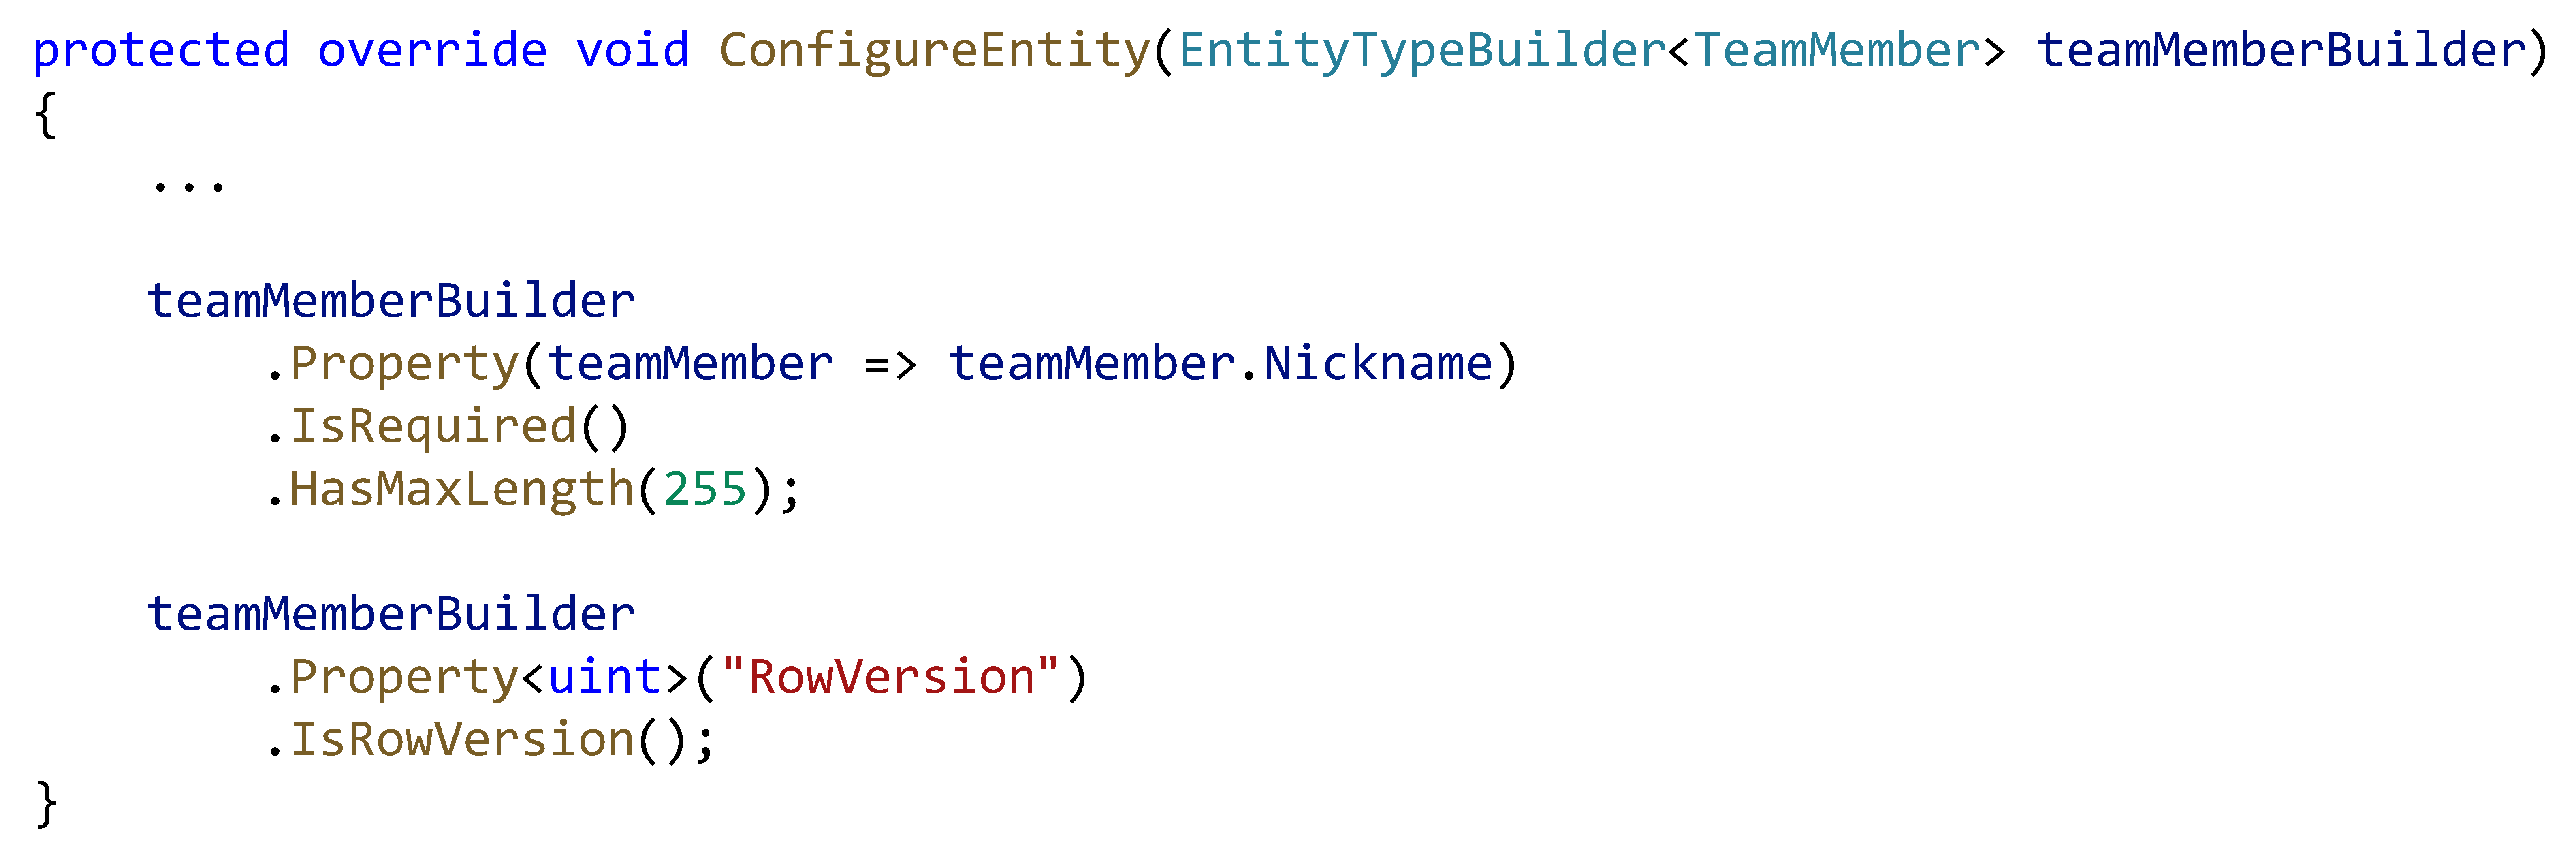
\includegraphics[width=\textwidth]{figures/concurrency-token.pdf}
    \caption{Code sample configuring EF Core (utilizing \texttt{IEntityTypeConfiguration} interface) to use a property of the \texttt{TeamMember} entity as a concurrency token. Note that the~code does not explicitly reference the property, but rather uses a shadow property, meaning the property exists in database as a column but does not exist in the domain object itself, and thus does not pollute the domain with properties with no business value.}
    \label{fig:concurrency_token}
\end{figure}

The concurrency token most probably does not need to be in every entity because the race condition may not always cause a problem, with regards to the \textit{TeamUp} application:
\begin{itemize}
    \item \texttt{User} entity needs a concurrency token as the entity has a \textit{NumberOfOwnedTeams} column used to solve the enforcing of the business rule (max number of owned teams) in a race condition when concurrently creating teams by the same user. The conflict with concurrent creation of users with the same email is solved by a unique constrain. 
    \item \texttt{Team} entity requires a concurrency token since this entity, similarly to the \texttt{User} entity, has a column (\textit{NumberOfMembers}) that is used to solve the enforcing of the business rule (max number of members) in a race condition when concurrently adding new members to the same team.
    \item \texttt{TeamMember} entity requires a concurrency token because concurrent requests to change a team ownership may leave the team with multiple owners.
    \item \texttt{Event} entity has to have a concurrency token as concurrent changes to the event may leave the record in an invalid state -- f.e., changes of start and end dates.
    \item \texttt{EventType} and \texttt{EventResponse} entities do not require a concurrency token since concurrent modification does not leave the system in an inconsistent state and data loss is irrelevant. The race condition resulting from concurrent creation of \texttt{EventResponse} is solved by a unique constraint on the composite index (\texttt{eventId} and \texttt{teamMemberId}).
    \item \texttt{Invitation} entity does not have mutable columns and concurrent creating of invitations is solved by a unique constraint on the composite index (\texttt{teamId} and \texttt{userId}).
\end{itemize}

Note that these solutions describe the clean architecture solution, the modular monolith solution is mostly the same, some entities are just split/copied into multiple db schemas.

\subsection{Integration Testing}
\label{dev:integration_testing}
In integration and end-to-end (E2E) testing, there is the question of whether to test with real service instances or in-memory mocks/versions, especially for testing database integration. 

The advantage of mocking service dependencies via in-memory alternatives is performance as tests run really fast and can be run in parallel. 

The disadvantage is that some services may not have in-memory versions (EF Core does provide option to use db context around in-memory database), moreover, the in-memory mocks-ups may differ from the real implementation (i.e. database transactions \dots) and therefore change the way the system works in testing and production.

For E2E testing, the application is tested with real instances of database and bus (for~modular monolith solution) and the mail server is mocked with in memory inbox. The~testing is implemented using \textbf{xUnit}\footnote{\url{https://xunit.net/}} as a testing framework and following libraries:
\begin{itemize}
    \item \textbf{TestContainers}\footnote{\url{https://testcontainers.com/}} for running docker containers of real services, such as postgres or RabbitMQ, and using them for E2E testing of the application.
    \item \textbf{FluentAssertions}\footnote{\url{https://fluentassertions.com/}} for providing a more natural way of specifying expected outputs.
    \item \textbf{Respawn}\footnote{\url{https://github.com/jbogard/Respawn}} by Jimmy Bogard for resetting database between tests.
    \item \textbf{Bogus}\footnote{\url{https://github.com/bchavez/Bogus}} for deterministic generation of fake testing data.
    \item \texttt{Microsoft.AspNetCore.Mvc.Testing} package providing ASP.NET Core application factory configurable for testing purposes and running it in-memory.
\end{itemize}

Using the xUnit's \textit{Collection Fixtures}, all E2E tests are run against the same services: the~backend, the database and the service bus. These services are initialized at the start and xUnit then runs all tests sequentially:
\begin{enumerate}[start=0]
    \item Init: reset database into initial state using the \textbf{Respawn} library, reset additional properties used for testing (inbox, counters, datetime provider and so on).
    
    \item \textbf{Arrange}: generate testing data using the \textbf{Bogus} library and custom extension methods on top of it, persist data into the database or use them as payload, authenticate.
    
    \item \textbf{Act}: send HTTP request against the tested endpoint of the app running in memory.
    
    \item \textbf{Assert}:
    \begin{itemize}
        \item Test correct HTTP response code and error response.
        \item Test correct response payload when requesting query using the \textbf{FluentAssertuions} library and the \textit{object graph comparison} feature.
        \item Test correct database state when requesting Command.
    \end{itemize}
\end{enumerate}

\begin{figure} [H]
    \centering
    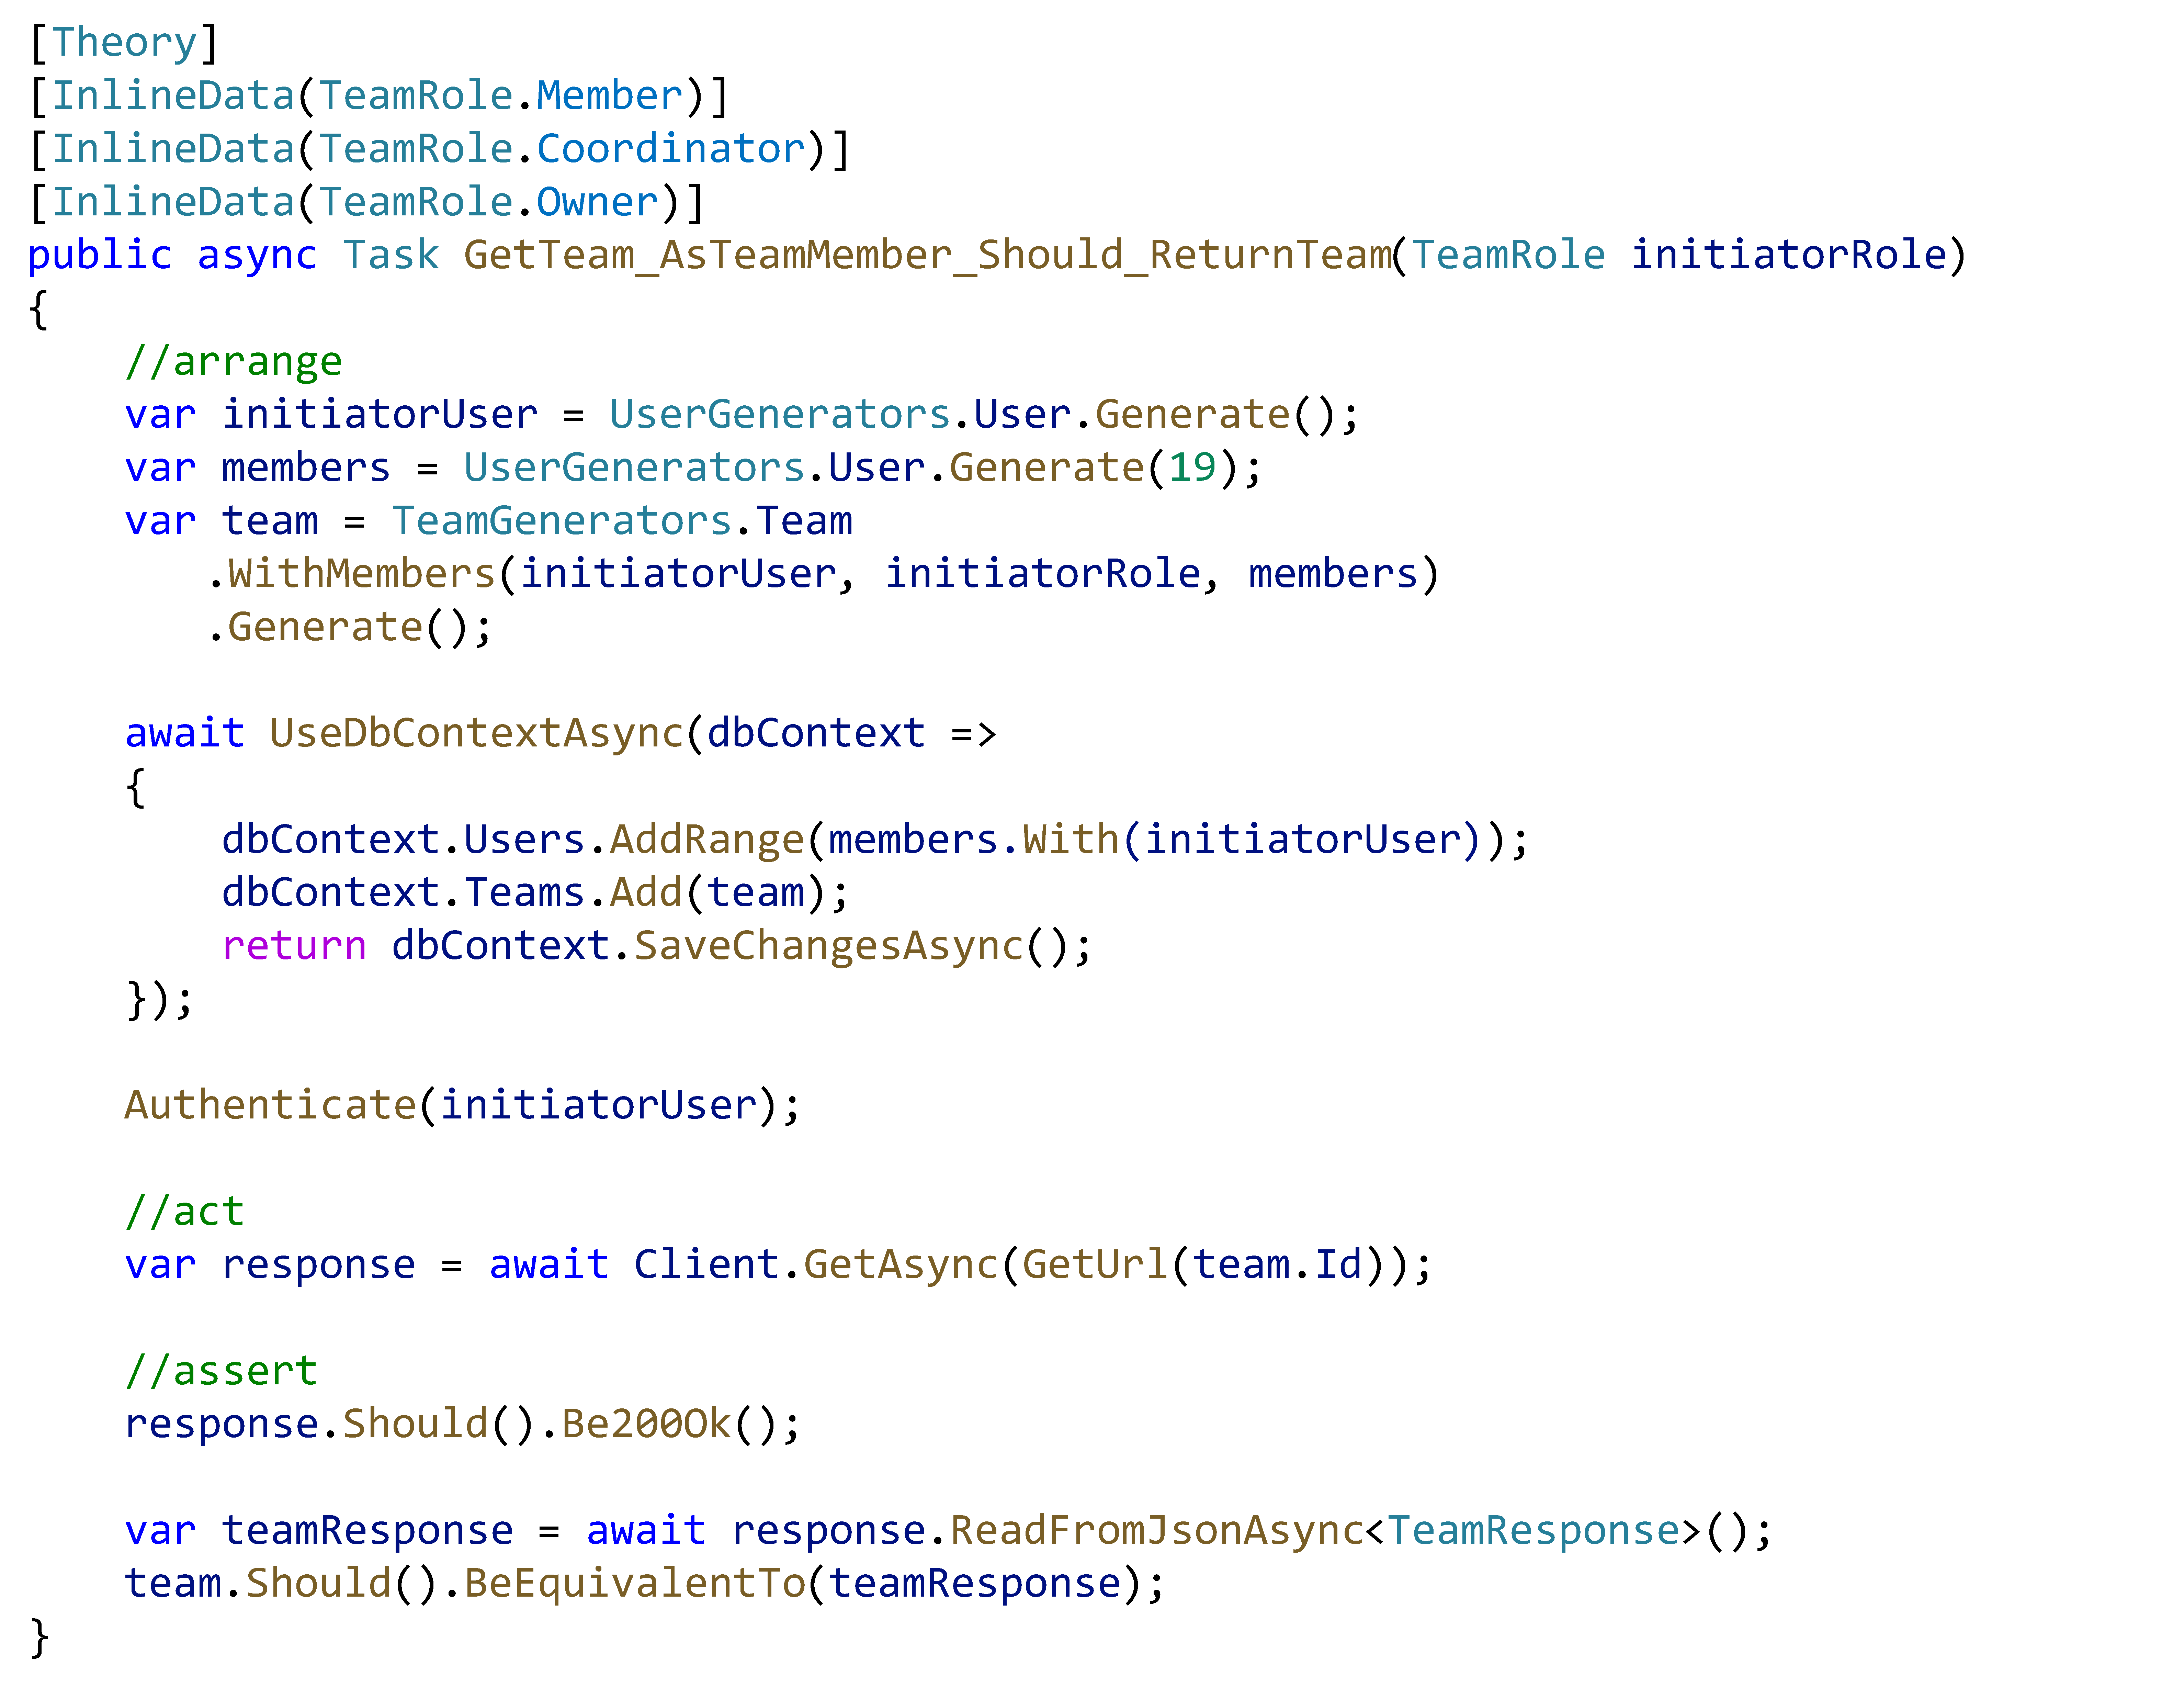
\includegraphics[width=\textwidth]{figures/endpoint-test.pdf}
    \caption{Code sample from the Clean Architecture solution of E2E test against a GET endpoint. Note that the test is written using the AAA pattern.}
    \label{fig:endpoint_test}
\end{figure}

\subsubsection{Testing Eventual Consistency}
The system consists of components that respond to a backend request with a delay and only after the request is completed, thus introducing eventual consistency (e.g. sending emails, but mainly propagating data between modules in the modular monolith). Testing eventual consistency might be challenging since waiting for a fixed amount of time may be inefficient and lead to nondeterministic test results.

In this case, the solution was to introduce callback invocations to desired components in~testing environment and wait for these callbacks after a request (with timeout to avoid livelock), where desired components are:
\begin{itemize}
    \item Outbox processor (background job) in the Clean Architecture solution, because after the outbox processing completes, the integration event raised by the request is handled or the handling has failed (test failed and caught a bug).
    
    \item Inbox consumer (called by background job) in the Modular Monolith solution with separate callback for each integration event handler invoked when successfully handled. In testing, it is necessary to specify for which (or multiple) integration event handler the test needs to wait (see figure \ref{fig:eventual_constistency_testing}).
\end{itemize}

The implementation of the callback mechanic uses the C-sharps \texttt{TaskCompletionSource<T>} feature\footnote{\url{https://learn.microsoft.com/en-us/dotnet/api/system.threading.tasks.taskcompletionsource-1}}, which enables the ability to wait for a result of a task (waiting for a callback) and set a result of that task from different/concurrent thread (invoking the callback).

\begin{figure} [H]
    \centering
    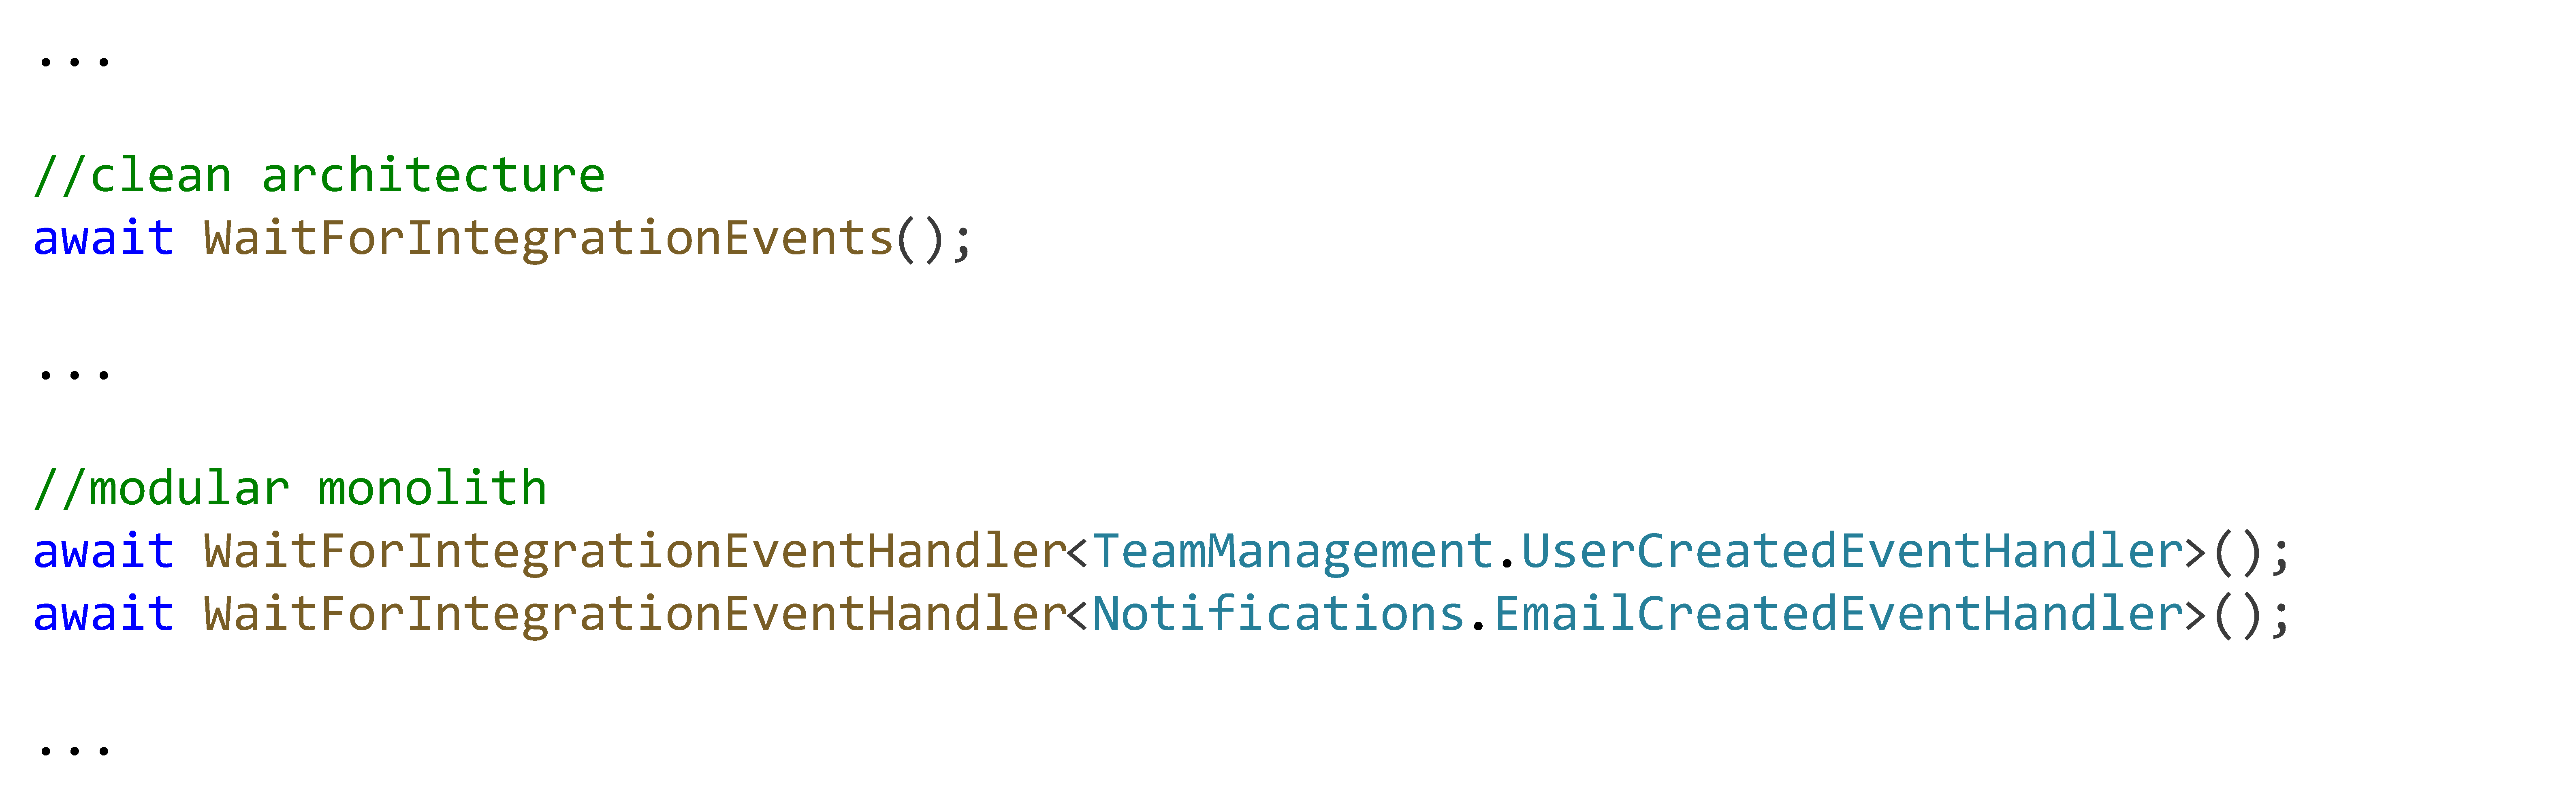
\includegraphics[width=\textwidth]{figures/eventual-consistency.pdf}
    \caption{Rough code example of the methods used in the solutions for waiting for the~completion of integration event handlers. Note that in the modular monolith, each module may have a handler for a given event, so a distinction by module needs to be used.}
    \label{fig:eventual_constistency_testing}
\end{figure}

\subsubsection{Testing Race Conditions}
To test that the measures against concurrency conflicts and race conditions (mentioned in~section \ref{dev:conccurency_conflicts}) work, it is necessary to be able to force a conflicting situation.

Using the previously mentioned callback mechanic, it is possible to adjust the \texttt{SaveChanges} method of the unit of work pattern that is used to persist changes and introduce \textit{before commit} and \textit{can commit} callbacks to enforce a conflicting situation (see figure \ref{fig:race_condition}). 

\begin{figure} [H]
    \centering
    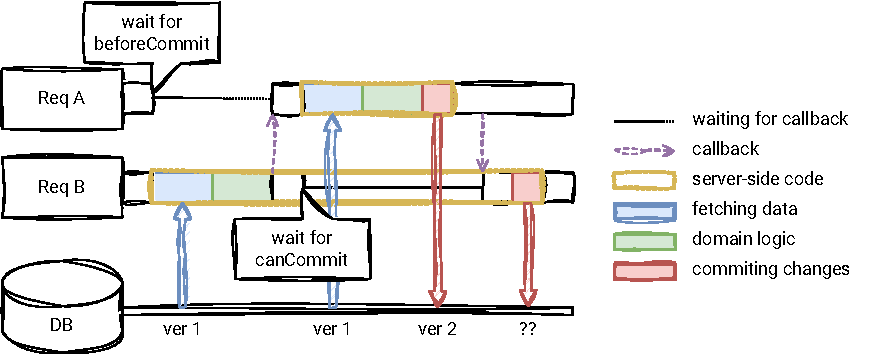
\includegraphics[width=\textwidth]{figures/race-condition.pdf}
    \caption{Diagram showing the enforcement of a conflicting situation between 2 requests by delaying committing changes of request B till request A is initiated and fully processed.}
    \label{fig:race_condition}
\end{figure}

\subsection{Architecture Testing}
\label{dev:arch_testing}
As the project grows, it is essential to ensure that all developers follow the architecture rules and DDD principles to take advantage of the architecture design and to avoid introducing bugs and unwanted coupling that would lead to the big ball of mud.

.NET compiler -- \textbf{Roslyn}\footnote{\url{https://github.com/dotnet/roslyn}} -- provides a powerful API surface for building code analysis tools and as such can be used to develop analyzers that flag violations of architecture rules and guidelines at compile time and subsequently suggest fixes. 

However powerful and versatile analyzers can be, their development is not cheap (in terms of knowledge) as a developer may need to understand static code analysis, compiler theory and framework for building the analyzers -- something that a traditional backend developer does not.

An alternative approach taken in the development of \textit{TeamUp} is to create tests using a~specialized library, such as \textbf{NetArchTest}\footnote{\url{https://github.com/BenMorris/NetArchTest}}, with a basic knowledge of reflection (known by a~generic backend developer) to test rules like:

\begin{itemize}
    \item dependency rules -- dependency of types in assembly/namespace on types from another assembly/namespace (i.e. clean architecture dependency tests, see figure \ref{fig:dependency_test}).
    
    \item type naming conventions -- e.g. a domain event must have a \textit{DomainEvent} suffix.
    
    \item type properties -- types have to be abstract/static/sealed/read-only etc.
    
    \item type existence -- for instance, class representing \texttt{Command} contain a nested validator.
    
    \item DI rules -- service can be injected only into certain classes (assuming injection via~constructors, i.e. query context can be injected only into query handlers).
    \\\dots
\end{itemize}

\begin{figure} [H]
    \centering
    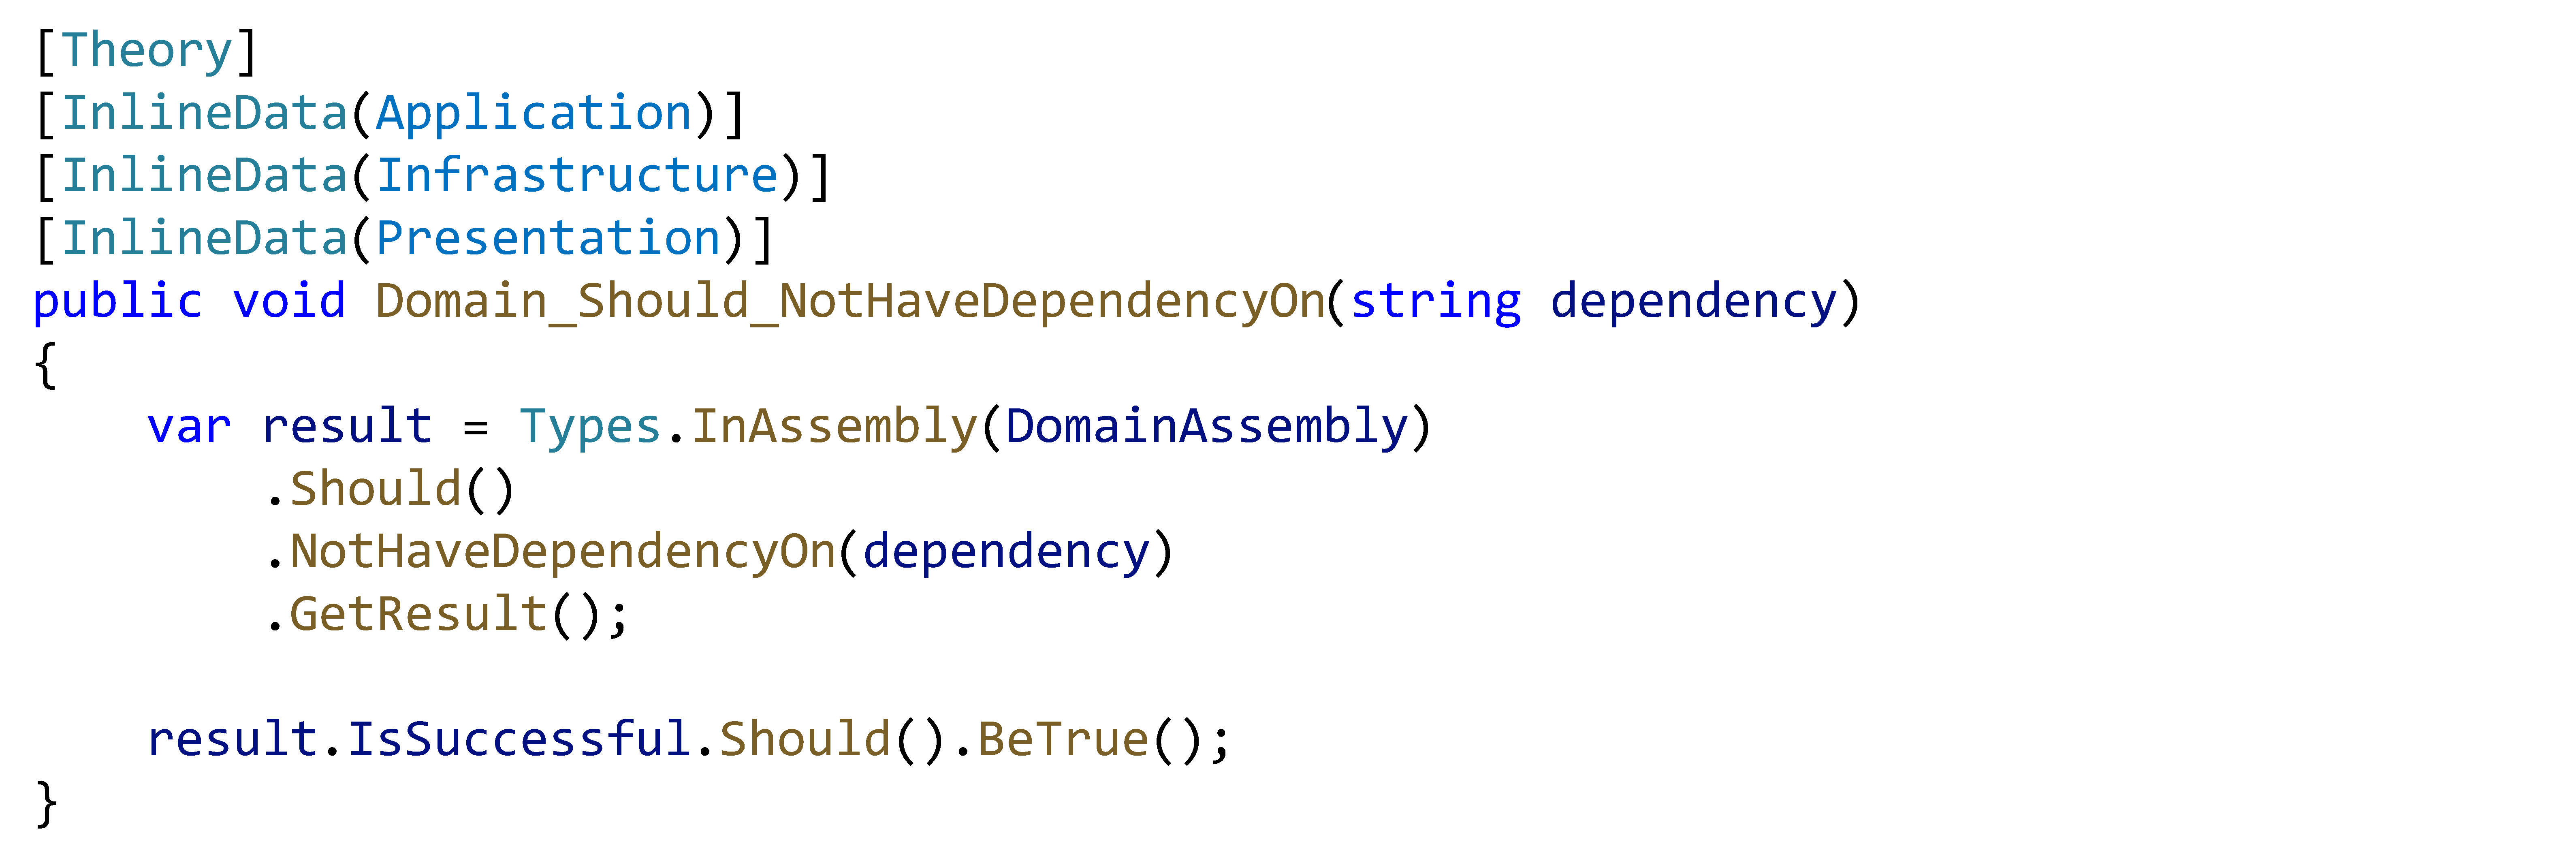
\includegraphics[width=\textwidth]{figures/dependency-test.pdf}
    \caption{Code sample of a dependency test from the Clean Architecture solution testing whether  the Domain layer depends on any types from the Application, Presentation, or Infrastructure layers. Noteworthy is that the Modular Monolith solution has more complex and more important dependency tests (see repository in section \ref{dev:modular_monolith}), as it has to follow more complex dependency rules to avoid the big ball of mud.}
    \label{fig:dependency_test}
\end{figure}

\chapter{Conclusion on selected architectures and their comparison}
\label{chapter_comparison}
This chapter summarizes my final thoughts on selected architectures -- Clean Architecture (section \ref{con:ca}) and Modular Monolith (section \ref{con:mm}) -- after developing a demo application in~both architectures while applying domain-driven design principles.

\section{Clean Architecture}
\label{con:ca}
The clean architecture is more modular than the traditional layered architectures, especially when integrating with external systems (databases, emailing services, etc.), providing easier exchangeability of such systems. Compare to more modular architectures, it may be difficult to implement larger systems.

The architecture does not really invite the application of DDD strategy design since it is difficult to implement/separate bounded contexts and in the demo application it seemed counterproductive to do so. However, the DDD tactical design is easily applicable and introduces positive effects on the system (rich domain, clear boundaries between entities, etc.).

From the way the clean architecture is interconnected, it is not the most suitable architecture for migrating to microservices.

The main advantage of clean architecture is the benefit of rapid development in early development stages while retaining decent maintainability as the system grows. Adding features to the system does change multiple layers, which limits development in larger/multiple teams. It is therefore not suitable for larger systems. 

In my opinion, the clean architecture together with DDD provides a good solution for mid-level information systems with basic modularity or for implementing modules (in a modular monolith) or services (in a microservice architecture). 

Given the scale of the demonstration application, its business complexity and technical requirements, a clean architecture with DDD tactical design and CQRS seems fitting.

\section{Modular Monolith}
\label{con:mm}
The modular monolith architecture excels in modularity (as the name suggests) and can match microservices in its ability to implement large-scale information systems.

The separation into modules works well with the DDD strategy design, as a module can represent a bounded context and the strict rules between modules mimic the nature of~bounded contexts. A module can then be implemented in whatever manner, but implementing modules using a clean architecture and DDD tactical design has proven itself.

Because a system is decomposed into modules similarly to microservice, the architecture can leverage its benefits for developer productivity in large/multiple teams and large information systems. The similarities with microservice architecture imply an easy (relatively speaking) transition to microservices, although it depends on the level of modularity and isolation chosen to implement a modular monolith.

Modular monolith introduces multiple complexities (as encountered in developing of demo application -- communication problems, eventual consistency complexity, etc.) and is still vulnerable to poor design choices, resulting in distributed monolith.

I am of the opinion that the modular monolith is the ideal starting architecture for~large enterprise-wide systems, however, it is uncommon to start building enterprise system out of nothing and it is hard to know whether a system becomes large-enough. Introducing this architecture for a smaller project (similar to microservices) brings unnecessary complexity.

The development of the demo application had not produced problems that a modular monolith is designed to solve, and the use of the modular monolith seemed excessive. Although some changes appeared cleaner/easier in the modular monolith (e.g. adding background services for cleaning invalid data), such occurrences were minimal and to properly see the benefits of modular monolith, either further experiments on the same application would need to be made, or a large-scale application in large teams would have to be developed (which is not coverable in a thesis).

Due to complexities in modular monolith, a more convenient approach might be to start a~project with a modular monolith architecture with a lower lever of modularity (in-process communication, etc., or even use a clean architecture) and later migrate to fully modular monolith with microservices-like aspects.

\chapter{Conclusion}
\label{chapter_conclusion}
\vspace{-2pt}
The aim of this thesis was to study and explore architectures for building modular monolithic information systems with domain-driven design and practically demonstrate two of~the~architectures on a chosen application.

The personal goal was to level-up my software engineering skills by studying currently popular architectures and accumulating additional knowledge on building information systems along the way, hence the scope of my own assignment.

In the context of meeting assignment objectives, I have:
\vspace{-7pt}
\begin{itemize}
    \item extensively studied the domain-driven design principles and explored several architectures for building modular information systems (1th objective);
    
    \item selected less and more modular architectures for deeper and practical exploration: Clean Architecture and Modular Monolith (2th objective);
    
    \item implemented demonstration application in both architectures and designed the domain using the DDD (3th objective), while continuously implementing end-to-end tests to validate correct functionality (4th objective extension);
    
    \item implemented frontend application to verify practical API usability of the backend solutions (4th objective) and introduced client-side cache (4th objective extension);
    
    \item summarized gathered experience on the selected architectures from the development process and stated my opinions in the context of application maintainability, extensibility, etc. in the penultimate chapter (5th objective).
\end{itemize}
\vspace{-5pt}
In addition, the thesis contains a chapter covering parts of the development process that are outside the main scope of the thesis, but still may be interesting to the potential reader.

To explore and analyse more of the architectures' capabilities, additional extensions/experiments can be performed on the implemented solutions, such as:
\vspace{-7pt}
\begin{itemize}
    \item Changing the core domain to support new functionalities.
    \item Adding features and new technologies (e.g. real-time notifications using web sockets) or changing supporting infrastructure technology (database, event-bus provider, etc.).
    \item Transitioning implemented solutions to microservices architecture.
\end{itemize}
\vspace{-50pt}


  % Bibliography
  % ----------------------------------------------

  \makeatletter
  \def\@openbib@code{\addcontentsline{toc}{chapter}{Bibliography}}
  \makeatother
  \bibliographystyle{bib-styles/Pysny/enplain}
%  \bibliographystyle{alpha}

  \begin{flushleft}
  \bibliography{bibliography}
  \end{flushleft}

  % Skip the page in the two-sided mode
  \iftwoside
    \cleardoublepage
  \fi

  % Appendices
  % ---------------------------------------------
  \appendix
\ifczech
  \renewcommand{\appendixpagename}{Přílohy}
  \renewcommand{\appendixtocname}{Přílohy}
  \renewcommand{\appendixname}{Příloha}
\fi
%  \appendixpage

% Skip the page in the two-sided mode
\iftwoside
  \cleardoublepage
\fi

  \ifczech
%    \section*{Seznam příloh}
%    \addcontentsline{toc}{section}{Seznam příloh}
  \else
%   \section*{List of Appendices}
%    \addcontentsline{toc}{section}{List of Appendices}
  \fi

  \startcontents[chapters]
  \setlength{\parskip}{0pt} 
  % list of appendices
  % \printcontents[chapters]{l}{0}{\setcounter{tocdepth}{2}}
  
  \ifODSAZ
    \setlength{\parskip}{0.5\bigskipamount}
  \else
    \setlength{\parskip}{0pt}
  \fi
  
 % Skip the page in the two-sided mode
  \iftwoside
    \cleardoublepage
  \fi
  
  % Appendices
  \chapter{Contents of the included storage media}

\dirtree{%
.1 /.
.2 Figures/.\DTcomment{created vector figures and original pictures taken}.
.2 Sources/.
.3 CleanArchitecture/.\DTcomment{clean architecture solution sources}.
.3 ModularMonolith/.\DTcomment{modular monolith solution sources}.
.3 Frontend/.\DTcomment{frontend solution sources}.
.2 Thesis/.\DTcomment{all thing necessary for building thesis pdf}.
.2 thesis.pdf.\DTcomment{this thesis in online format}.
.2 README.md.\DTcomment{basic information about the repository}.
.2 .gitmodules.
}

\chapter{Application Screenshots}

\begin{figure} [H]
    \centering
    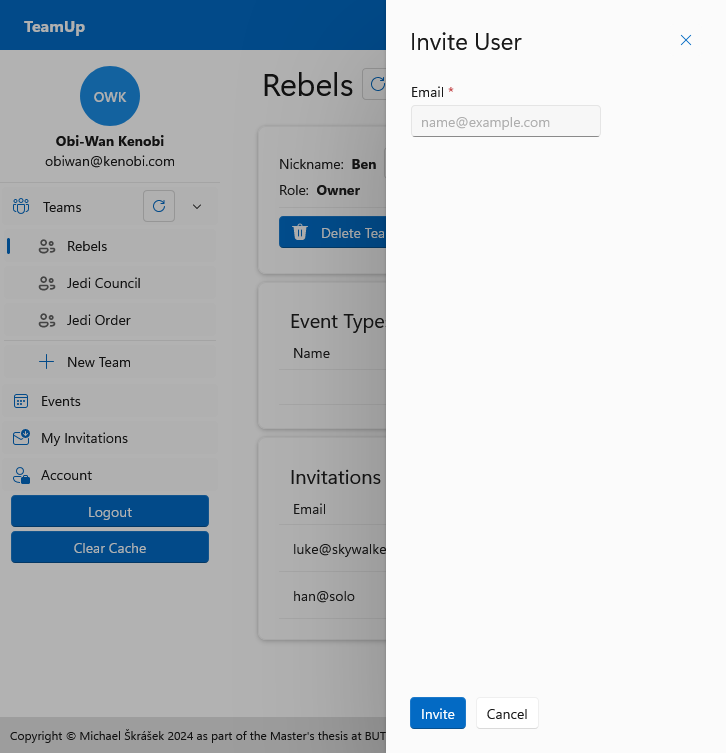
\includegraphics[width=0.95\textwidth]{figures/screenshot-invite.png}
    \caption{Screenshot of the invite user prompt panel.}
\end{figure}

\begin{landscape}
    \begin{figure} [H]
        \centering
        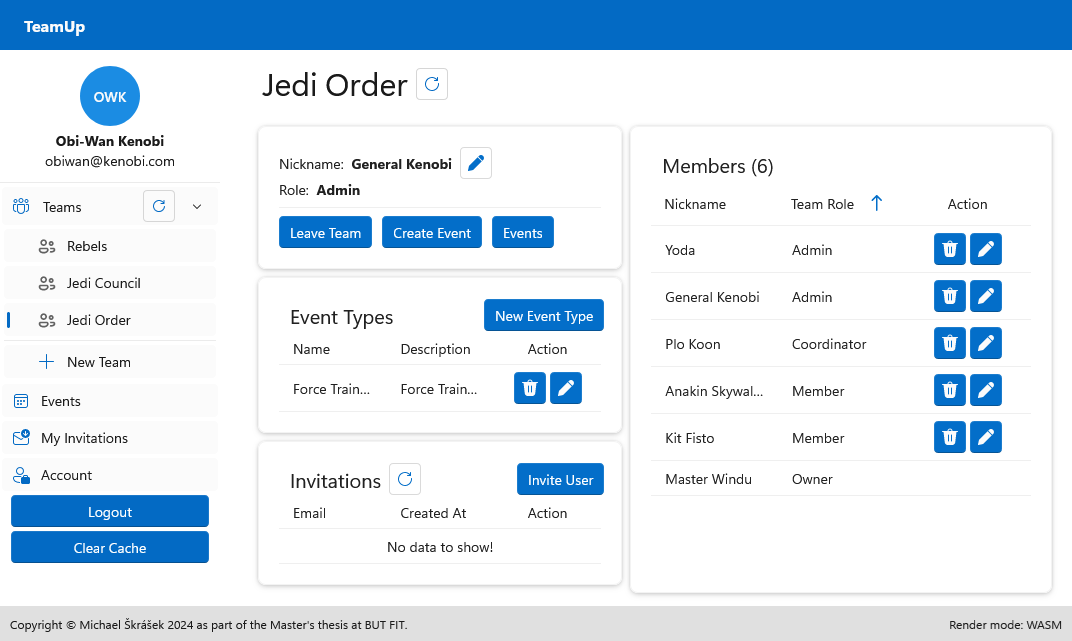
\includegraphics[height=0.85\textheight]{figures/screenshot-team.png}
        \caption{Screenshot of the team management page.}
    \end{figure}

    \begin{figure} [H]
        \centering
        \includegraphics[height=0.93\textheight]{figures/screenshot-team-events.png}
        \caption{Screenshot of the team events page.}
    \end{figure}
\end{landscape}

  
\end{document}
